\chapter{Analysis Strategy: Higgs $\to \tau\tau$}

This chapter describes a study of Higgs Boson production and subsequent
decay to a pair of $\tau$ leptons using CMS proton-proton collision data gathered in 2016.  This is the first
$\htt$ analysis performed using center-of-mass energy 13 TeV data from the LHC. Combining
these 13 TeV results with 7 TeV and 8 TeV CMS $\htt$ results we produce
the first single experiment observation of the $\htt$ process, observed at the 5.9 $\sigma$
confidence level.  Additionally, this study provides the strongest constraints on VBF Higgs 
production to date for all CMS Higgs Boson analyses.

\section{Overview: Higgs $\to \tau\tau$}

This chapter specifically focuses on studying the Higgs Boson produced via the gluon fusion
or the VBF production mechanisms.  A study of the Higgs Boson produced in associated production with
$\PW/\PZ$ is presented in the following chapter~\ref{sec:vh_analysis}. This study utilizes the
full 2016 $\pp$ dataset collected by CMS corresponding to 35.9$\fbinv$ of integrated luminosity.
In the following pages the symbol $\ell$ refers to electrons and muons and $\tauh$ refers to hadronically
decaying $\tau$ leptons.  We study all possible $\tau\tau$ final state combinations with the
exception of two electron and two muon final states because of the low 
$\tau\tau \to \tau_{e}\tau_{e}/\tau_{\mu}\tau_{\mu}$
branching fractions and high background from $\PZ \to ee/\mu\mu$.  The $\htt$ final states which are
studied are: $\tau_{e}\tauh$ denoted here as $\Pe\tauh$, $\tau_{\mu}\tauh$ denoted as $\Pgm\tauh$,
$\tau_{e}\tau_{\mu}$ denoted here as $\Pe\Pgm$, and lastly, $\tauh\tauh$ denoted as $\tauh\tauh$.
This combination of final states covers about 94\% of all possible $\tau\tau$ final states.
The different $\tau\tau$ final states will be refered to as different channels in the following pages.
We ensure uniqueness between the four studied channels be applying veto criteria to events based
on the number of reconstructed and loosely identified electrons and muons.  This ensures that 
no data or simulated event is double counted in two channels.

Selected events are classified into three different categories targeting different characteristics
of the gluon fusion and VBF production topologies.  The categories are defined according to the
number and kinematics of the associated jets in each event along with the reconstructed $\pt^{Higgs}$.
A number of different control regions are used in the final fit for signal extraction.  This allows
the fit to simultaneously adjust and constrain all processes targeted by a control region.  This is in
contrast to extracting a scale factor which is applied as a fixed value in an analysis and not
allowed to adjust as other background process adjust in the final fit.  The backgrounds which are
targeted with dedicated control regions are: $\PW$+jets, QCD, and $\ttbar$.



\subsection{Event Selection}

There are specific baseline criteria applied to all electrons, muons, $\tauh$, and jets for every
event.  Depending on the final state, additional requirements are placed on these objects based
on combination or trigger requirements and analysis optimization.  The baseline criteria ensure
that each object is well reconstructed and well identified and consistent with the analysis
strategy. 

\subsection{Triggers}
Selected events are required to to have fired a trigger consisten with their categorized final
state channel.  For the $\Pgm\tauh$ channel, events are selected using a combination
of a single isolationed muon trigger as well as a cross trigger firing on an isolated muon and
an isolated $\tauh$.  The $\Pgm\tauh$ cross trigger allows for a lower possible $\pt$ threshold
on the selected muon.  In contrast, due to the HLT menu available in 2016, the $\Pe\tauh$ cross triggers
do not bring a substantial increase in acceptance and were not used in this analysis.
For the $\Pe\tauh$ channel, events are selected using only a trigger firing on a 
single isolated electron.  For the $\Pe\Pgm$ channel, events are selected with electron-muon corss
triggers requiring an isolated online electron and an isolated online muon.  There are two 
different electron-muon corss triggers used with their HLT $\pt$ thresholds detailed following.
For the $\tauh\tauh$ channel, events are selected using an online criteria of two loosely isolated $\tauh$.  
The high level trigger paths used and their online $\pt$ thresholds are detailed in table~\ref{tab:htt_hlt_triggers}.

Due to changing running conditions and a changing HLT menu throughout 2016 data taking, the HLT path
requirements change throughout 2016 and are era dependant.  The study avoids using any prescaled
HLT paths; during latter eras, at higher instantaneous luminsity, some HLT paths became diabled
or prescaled.  When this happens we avoid using that specific trigger for the given prescaled/disabled
era.  For the $\Pgm\tauh$ channel this 
leads to changes in the $\abs\eta$ requirement on the online muon in the single muon triggers.
There are two muon-tau cross triggers available throughout 2016.  One of them requires only the
presence of a single muon at the Level-1 trigger and has ``SingleL1'' appended to its path
name.  The other one requires the presence of both a muon and a $\tauh$ at the Level-1 trigger.
The single electron trigger used in the $\Pe\tauh$ channel remained constant through the year.
Due to changing pileup conditions and increasing luminosity during the final eras, the online
isolation criteria was changed for the $\tauh\tauh$ channel triggers.  The online $\tauh$ 
isolation changed from being based on purely charged energy deposits to being based on a 
combination of charged and neutral based energy deposits.  The triggers useded in the
$\Pe\Pgm$ channel changed during the final two eras, G and H, and had a lepton DZ filter
applied to them.  The DZ filter requires that the electron and muon match to the HLT primary
vertex and is a common method used to reduce rate at the HLT.  In all channels, the electrons, muons, and
$\tauh$ in each event must be matched to within $\Delta R < 0.5$ with the associated
HLT object which triggerd the event.


\begin{table*}[htbp]
\centering
\begin{footnotesize}
%\begin{scriptsize}
\begin{tabular}{|l|l|l|l|}
\hline
  Channel           &         Trigger $\pt$ Req.              &     High Level Trigger Path  &   Eras  \\
\hline
  $\mu\tauh$       &         $\Pgm(22)$                     &  \scriptsize{HLT\_IsoMu22\_v*} & B-F  \\ 
                   &         $\Pgm(22)$                     &  \scriptsize{HLT\_IsoTrkMu22\_v*} & B-F   \\ 
                   &         $\Pgm(22)$                     &  \scriptsize{HLT\_IsoMu22\_eta2p1\_v*} & C-H  \\
                   &         $\Pgm(22)$                     &  \scriptsize{HLT\_IsoTrkMu22\_eta2p1\_v*} & C-H   \\
                   &         $\Pgm(19)\,\&\,\tauh (21)$     &  \scriptsize{HLT\_IsoMu19\_eta2p1\_LooseIsoPFTau20\_SingleL1\_v*} &  All Eras  \\
                   &         $\Pgm(19)\,\&\,\tauh (21)$     &  \scriptsize{HLT\_IsoMu19\_eta2p1\_LooseIsoPFTau20\_v*} &  All Eras \\
\hline
  $\Pe\tauh$       &         $\Pe (25)$                     &  \scriptsize{HLT\_Ele25\_eta2p1\_WPTight\_Gsf\_v*}   & All Eras \\
\hline
 $\tauh\tauh$      &         $\tauh (35)\,\&\,\tauh (35)$   &  \scriptsize{HLT\_DoubleMediumIsoPFTau35\_Trk1\_eta2p1\_Reg\_v*} & B-G   \\ 
                   &         $\tauh (35)\,\&\,\tauh (35)$   &  \scriptsize{HLT\_DoubleMediumCombinedIsoPFTau35\_Trk1\_eta2p1\_Reg\_v*} & H  \\
\hline
  $\Pe\Pgm$        &         $\Pe(12)\,\&\,\Pgm (23)$       &  \scriptsize{HLT\_Mu23\_TrkIsoVVL\_Ele12\_CaloIdL\_TrackIdL\_IsoVL\_v*} & B-F \\
                   &         $\Pe(12)\,\&\,\Pgm (23)$       &  \scriptsize{HLT\_Mu23\_TrkIsoVVL\_Ele12\_CaloIdL\_TrackIdL\_IsoVL\_DZ\_v*} & G-H  \\
                   &         $\Pe(23)\,\&\,\Pgm (8)$        &  \scriptsize{HLT\_Mu8\_TrkIsoVVL\_Ele23\_CaloIdL\_TrackIdL\_IsoVL\_v*} & B-F  \\
                   &         $\Pe(23)\,\&\,\Pgm (8)$        &  \scriptsize{HLT\_Mu8\_TrkIsoVVL\_Ele23\_CaloIdL\_TrackIdL\_IsoVL\_DZ\_v*} & G-H  \\
\hline
\end{tabular}
\end{footnotesize}
%\end{scriptsize}
\caption{For each channel the online HLT $\pt$ threshold is listed along with the specific associated
HLT paths.  Through out 2016 data taking, the HLT menu changed to respond to changing online
conditions at CMS and the LHC.  This is reflected in progressivly tighter triggers
being available towards the end of the 2016 run.
\label{tab:htt_hlt_triggers}
}
\end{table*}



\subsection{Baseline Object Selection}
All electrons and muons must meet the minimum requirement
that the distance of closest approach to the primary vertex satisfies $\abs{d_z}<0.2$ cm
along the beam direction, and $\abs{d_{xy}}<0.045$ cm in the transverse plane. Ensuring
compatibility with the primary vertex is consistent with the predicted infinitesimal life-time of
a Higgs Boson. The HPS reconstruction of $\tauh$ detailed in section~\ref{sec:XXX} can involve
combining together multiple tracks and $\PGpz$s coming from intermediary $\tau$ decay products.
Due to these intermediary products, the reconstructed $d_{xy}$ for $\tauh$ are often
larger than those for electrons and muons.  Because of this, the primary vertex matching
criteria are relaxed for $\tauh$ and only require $\abs{d_z}<0.2$ cm.

The offline selection criteria for all electrons, muons and $\tauh$ are motivated and constrained
by the High Level Trigger requirements of their path.  Specifically, the offline $\pt$ criteria
applied are always higher than the HLT $\pt$ threshold to ensure a stable measurement and application
of trigger efficiencies.  An offline $\pt$ threshold applied right at the HLT $\pt$ threshold
makes measurement of the steeply rising efficiency at the HLT threshold absolutly critical.
This is very difficult to do perfectly and would lead to very large trigger systematics
at low $\pt$ in the turn-on region.  Additionally, there are offline $\eta$ restrictions
enforced which align with those at the HLT.

All selected electrons, muons, and $\tauh$ must be well identified and isolated from overlapping
energy deposits and reconstructed objects.  This study uses identification criteria
provided centrally by the CMS Physics Object Groups.  All identification and isolation
working points following have been selected through an optimization process selecting
for increased analysis sensitivity.  The optimimum working points strike a balance
between signal efficiency and background rejection.  For electrons an MVA-based ID
is used in both the $\Pe\tauh$ and $\Pe\Pgm$ channels which has been tuned to provide 
80\% electron selection efficiency.  Muons in both the $\mu\tauh$ and $\Pe\Pgm$ channels
the Particle Flow Medium ID is required.  The selection of $\tauh$ relies on MVA-based working
points.  The $\tauh$ MVA-based working points combine both object identification and object
isolation together into a single set of working points.  Table~\ref{tab:htt_obj_selection}
details the $\pt$, $\abs\eta$, identification and isolation criteria for all electrons, muons,
and $\tauh$ selected in the study.


\begin{table*}[htbp]
\centering
\begin{small}
\begin{tabular}{l|l|l|l|l}
  Channel       & $\pt$ ($\GeV$) & $\eta$ & Identification & Isolation \\
\hline
  $\mu\tauh$       &   $\pt^\Pgm>20$     &  $\abs{\eta^\Pgm}<2.1$    &   PF ID Medium &  $I^{\Pgm}<0.15$       \\
                   &   $\pt^{\tauh}>30$  &  $\abs{\eta^{\tauh}}<2.3$ &   MVA $\tauh$ ID  & MVA $\tauh$ ID \\
\hline
 $\tauh\tauh$      &   Leading $\pt^{\tauh}>50$ & $\abs{\eta^{\tauh}}<2.1$  &    MVA $\tauh$ ID    & MVA $\tauh$ ID    \\
                   &   Subleading $\pt^{\tauh}>40$ & $\abs{\eta^{\tauh}}<2.1$  &    MVA $\tauh$ ID & MVA $\tauh$ ID    \\
\hline
  $\Pe\tauh$       &   $\pt^\Pe>26$      & $\abs{\eta^\Pe}<2.1$       &   MVA 80\% WP  &  $I^{\Pe}<0.1$  \\
                   &   $\pt^{\tauh}>30$  &  $\abs{\eta^{\tauh}}<2.3$  &   MVA $\tauh$ ID & MVA $\tauh$ ID \\
\hline
  $\Pe\Pgm$        &   $\pt^{\Pe}>13$    & $\abs{\eta^\Pe}<2.5$   &   MVA 80\% WP   & $I^{\Pe}<0.15$   \\
                   &   $\pt^{\Pgm}>15$   & $\abs{\eta^\Pgm}<2.4$  & PF ID Medium &  $I^{\Pgm}<0.2$    \\
\hline
\end{tabular}
\end{small}
\caption{Kinematic, identification and isolation selection requirements for the four di-$\Pgt$ channels.
\label{tab:htt_obj_selection}
}
\end{table*}


The three different signal extraction categories rely on the details of reconstructed jets, or
lack there of, in each event.  Jets are reconstructed using the anti-$k_{\text{T}}$ algorithm with distance
parameter $\Delta\text{R}=0.4$~\cite{Cacciari:2008gp}.  Charged hardons that are not consistent with
the primary vertex are removed from the anti-$k_{\text{T}}$ clustering.  Jets are only considered
if they pass they pass the loose working point of the PF Jet ID discriminator~\cite{jetID}.
Jets must have $\pt > 30 \GeV$ and $\abs\eta<4.7$.  The $\pt$ and $\eta$ requirements are altered
for cases where the jet is identfied as having likely originated from a b-quark.  Jets likey originating
from a b-quark are considered if they pass the CISVv2 Medium working point are then tagged as b-tagged jets.
B-tagged jets have a relaxed $\pt$ requirement but much tighter $\eta$ requirement of $\pt > 20 \GeV$ 
and $\abs\eta<2.4$.  The tightened $\eta$ requirment necessitates that b-tagged jets are located within
the detector volumne fully covered by the CMS pixel and strip tracker.
Lastly, all jets must be separated from the selected electrons, muons, and $\tauh$ by $\Delta\text{R}>0.5$.

Depending on the di-$\tauh$ channel, there are specific topological cuts targeted at significantly
reducing the contribution of certain background processes in the signal region.  The large $\PW+\text{jets}$
cross section combined with a non-negligible jet $\to \tauh$ fake rate leads to a large $\PW+\text{jets}$
contribution in the $\ell\tauh$ channels.  This contribution is significantly reduced at the cost of
minimal signal events by cutting on the transverse mass, $\MT$.  Where the $\MT$ selection is defined as

\begin{equation}
\MT \equiv \sqrt{\smash[b]{2 \pt^\ell \ptmiss [1-\cos(\Delta\phi)]}} < 50\GeV,
\end{equation}

where $\pt^\ell$ is the transverse momentum of the lepton $\ell$,
and $\Delta\phi$ is the azimuthal angle between its direction and the \etvecmiss.

FIXME - Add MT plot from ZTT paper?

In the $\Pe\Pgm$ channel, the large \ttbar background is reduced by requiring 
$p_\zeta - 0.85 \, p_\zeta^{\text{vis}} > -35$ or $-10$\GeV depending on which category the event is
classified within.  $p_\zeta$ is the component of the \etvecmiss projected along the bisector 
of the transverse momenta of the two leptons and $p_\zeta^{\text{vis}}$ is the sum of the components 
of the lepton transverse momenta along the same direction~\cite{Khachatryan:2014wca}, also see
figure~\ref{fig:htt_pZeta} for visual reference.
This $p_\zeta$ selection criteria has a high signal efficiency because the \etvecmiss is typically oriented
in the same direction as the visible di-$\Pgt$ system in signal events because the \etvecmiss is 
the results of neutrinos from the signal $\tau$s.  The orientation of the \etvecmiss with respect
to the di-$\tau$ system is much less predictable in \ttbar events.  In addition, events with a b-tagged 
jet are discarded to further suppress the \ttbar background in the $\Pe\Pgm$ channel.

\begin{figure*}[htbp]
\centering
     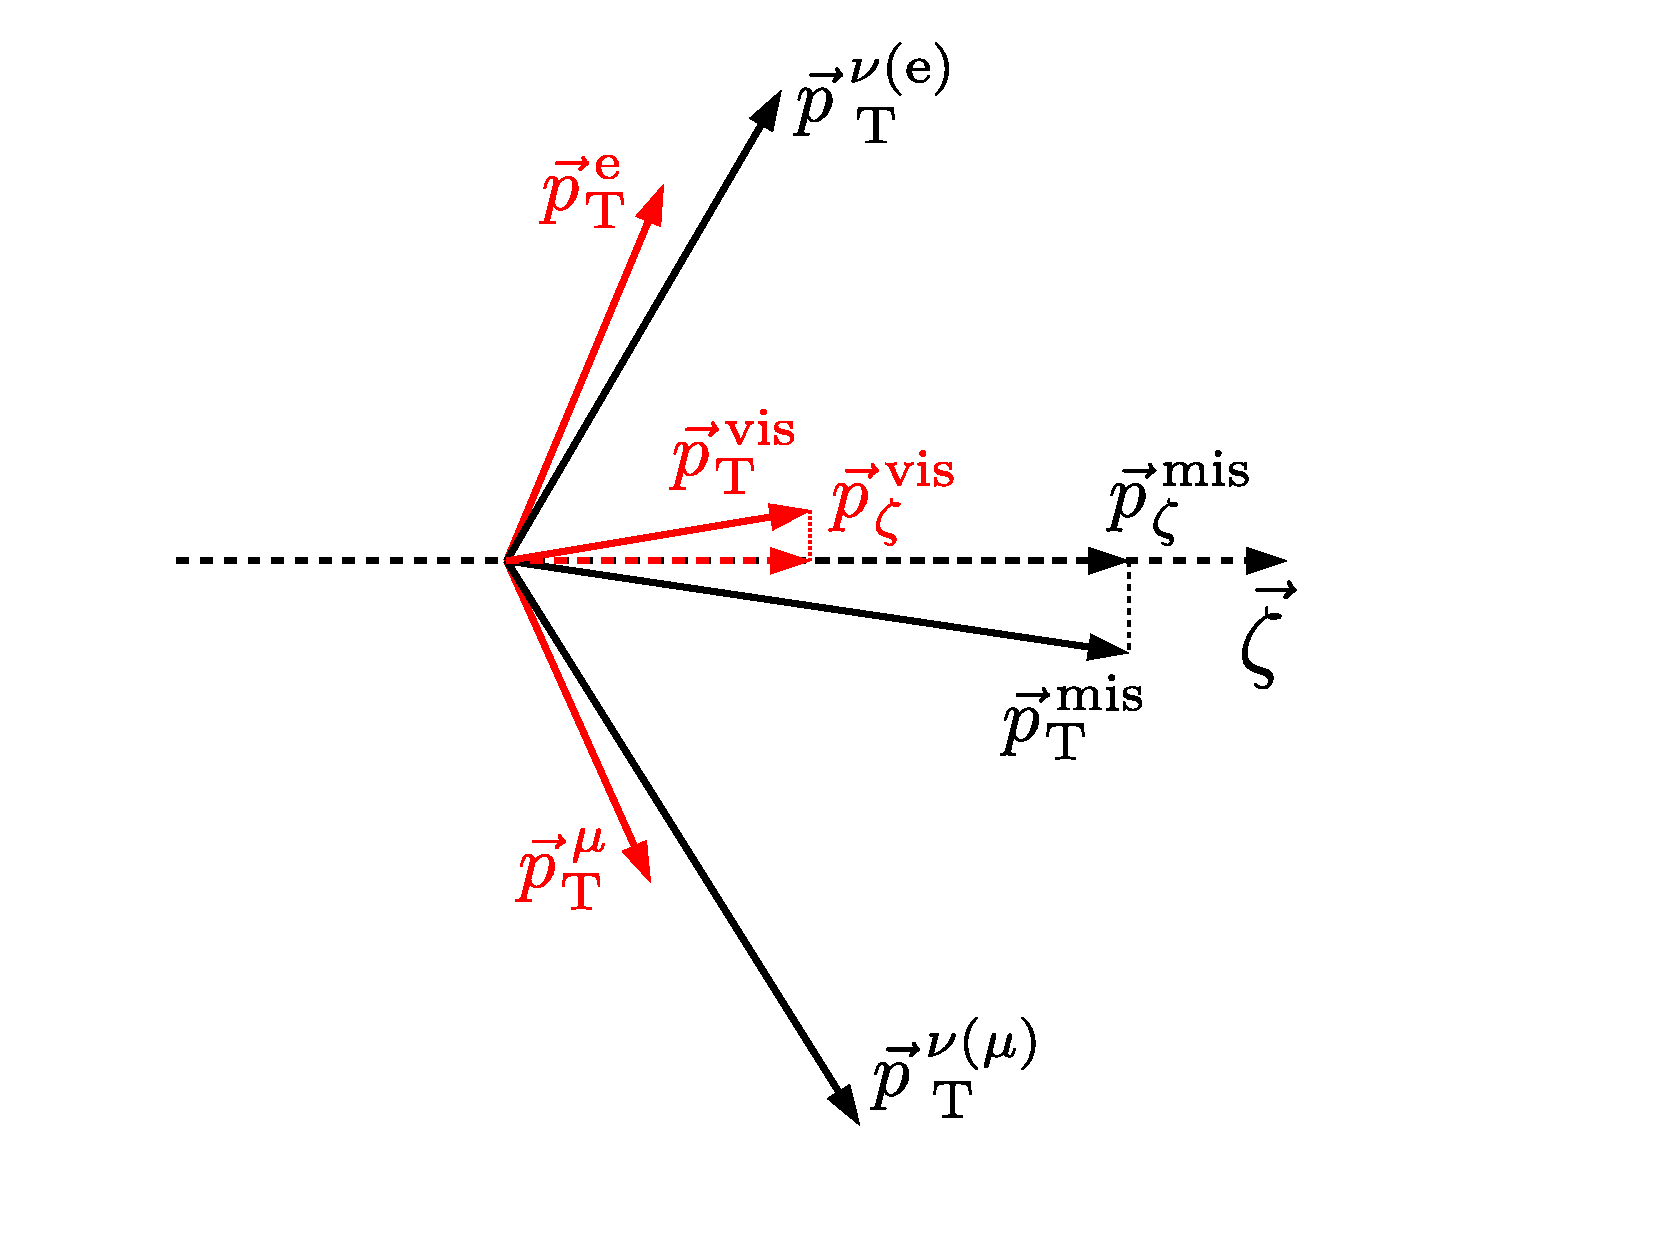
\includegraphics[width=0.4\textwidth]{higgs_to_taus/plots/pZeta_def.pdf}
     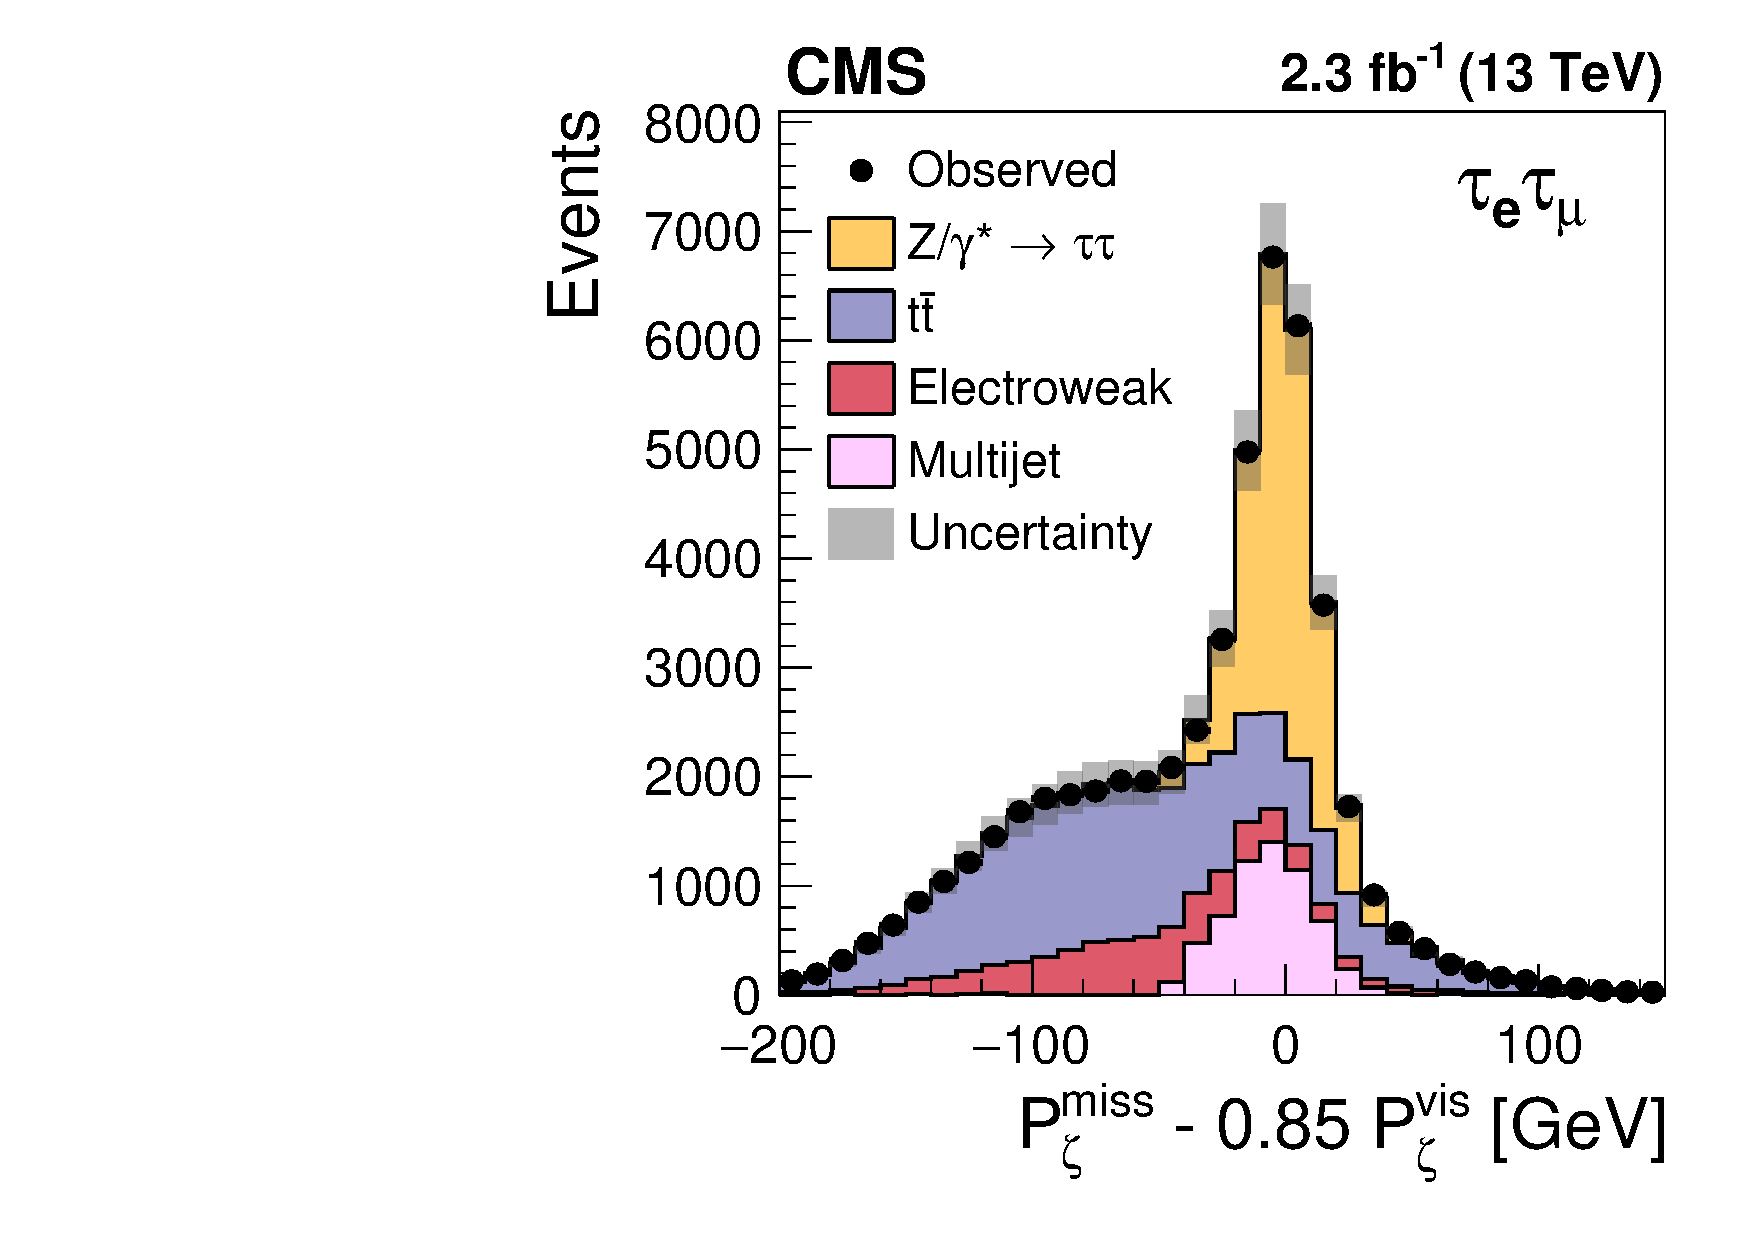
\includegraphics[width=0.4\textwidth]{higgs_to_taus/plots/htt_em_pZeta.pdf}\\
     \caption{
(Left) Diagram showing the construction of the $p_\zeta$ and $p_\zeta^{\text{vis}}$ projections.
(Right) An example $p_\zeta - 0.85 \, p_\zeta^{\text{vis}}$ distribution is shown for a similar but not
overlapping selection in the $\Pe\Pgm$ channel.  This distribution is from an analysis focusing on specifically studying the
$\PZ\to\tau\tau$ process~\ref{HIG-15-007}.
In the $\htt$ analysis, the Higgs Boson $p_\zeta - 0.85 \, p_\zeta^{\text{vis}}$
spectrum aligns very closely with the $Z\to\tau\tau$ distribution shown here.
     }
     \label{fig:htt_pZeta}
\end{figure*}

\subsection{Categorization}

Selected events are split into three mutually exclusive categories per decay channel.
The categories are designed to target different aspects of the gluon fusion and VBF Higgs Bosont production mechanisms.
In each category the two variables that maximize the $\PH\to\Pgt\Pgt$ sensitivity are chosen to build 
two-dimensional (2D) distributions.

The three categories are defined as:
\begin{itemize}
\item {0-jet}: This category targets Higgs Boson events produced via gluon fusion.
The two variables chosen to extract the results are $\mvis$ and
the reconstructed $\tauh$ decay mode in the $\Pgm\tauh$ and $\Pe\tauh$ decay channels.
In the $\Pe\Pgm$ channel, $\mvis$ and the $\pt$ of the muon are used.  The $\PZ\to\ell\ell$ background 
is large in the 1-prong and 1-prong + $\PGpz$(s) $\tauh$ decay modes in the
$\Pgm\tauh$ and $\Pe\tauh$ channels.  By using only $\mvis$ instead of $\mtt$ the \etvecmiss
does not smear the mass reconstruction for $\PZ\to\ell\ell$ and retains a nice sharp peak.
The shape Z $\mvis$ peak of $\PZ\to\ell\ell$ provides 
an excellent handel to distinguish $\PZ\to\ell\ell$ from the other background process and
helps constrain the associated uncertainties for electrons and muons faking $\tauh$.
As electrons and muons almost exclusively fake 1-prong 1-prong + $\PGpz$(s) $\tauh$,
the reconstructed $\tauh$ decay mode is used as the second of the 2D variables in the
$\Pgm\tauh$ and $\Pe\tauh$ channels.  Additionally, the lack of $\PZ\to\ell\ell$ in the
3-prong decay mode results in increased signal significance.
Examples of the 2D distributions for the signal and $\PZ\to\ell\ell$ background
in the 0-jet category of the $\Pgm\tauh$ decay channel are shown in Fig.~\ref{fig:htt_2Dcategories} (top).
In the $\tauh\tauh$ decay channel, only one observable, $\mtt$, is considered because of the low i
event yields due to the relatively high $\pt$ thresholds on the $\tauh$ at trigger level, and 
because of the sharply falling $\tauh$ $\pt$ distribution.  Simulations indicate that about 98\% 
of signal events in the 0-jet category correspond to Higgs Bosons produced via the gluon 
fusion production mechanism.\\

\item {VBF}: This category targets Higgs boson events produced via the VBF process.
The presence of jets from the hard scattering process in VBF production leads the study to heavily
utilize jet kinematics and the jet topology in the VBF category.
Events are selected with at least two (exactly two) jets with $\pt>30$\GeV in the
$\tauh\tauh$, $\Pgm\tauh$, and $\Pe\tauh$ ($\Pe\Pgm$) channels.
In the $\Pgm\tauh$, $\Pe\tauh$, and $\Pe\Pgm$ channels, the two leading jets are required to have 
an invariant mass, $\mjj$, larger than 300\GeV. The variable $\pth$, defined as the magnitude 
of the vectorial sum of the $\ptvec$ of the visible decay products of the $\Pgt$ leptons 
and $\etvecmiss$, is required to be greater than 50 (100)\GeV in the $\Pgm\tauh$
 and $\Pe\tauh$ ($\tauh\tauh$) channels to reduce the contribution from $\PW+\text{jets}$ 
backgrounds. This selection criterion also suppresses the background from quantum 
chromodynamics (QCD) multijet events. In addition, the $\pt$ threshold on the $\tauh$ 
candidate is raised to 40\GeV in the $\Pgm\tauh$ channel, and the two leading jets in the 
$\tauh\tauh$ channel should be separated in pseudorapidity by $\Delta\eta>2.5$. The $\Delta\eta>2.5$
cut in the $\tauh\tauh$ channel significantly reduces the contributions QCD events at the cost
of very few signal events because of the large jet $\Delta\eta$ in true VBF events.
The two observables used in the VBF category are $\mtt$ and $\mjj$ for all channels. Example 2D 
distributions for the signal and $\PZ\to\Pgt\Pgt$ background
in the VBF category of the $\Pgm\tauh$ decay channel are shown in Fig.~\ref{fig:htt_2Dcategories} (center). 
Integrating over the whole $\mjj$ phase space, up to 57\% of the signal events in the VBF 
category are produced in the VBF production mode, but this proportion increases with $\mjj$ allowing
for signal production process discrimination in the highest $\mjj$ ranges.\\

\item {Boosted}: This category contains all selected events that do not enter one of the previous 
categories, namely events with one jet and events with several jets that fail the specific requirements of the VBF category.
The Boosted category contains a mix of gluon fusion events produced in association with one or more jets (78--80\% of signal events),
VBF events where one of the jets escaped detection or has low $\mjj$ (11--13\%), as well as
Higgs bosons produced in association with a $\PW$ or a $\PZ$ boson decaying hadronically (4--8\%).
Because these gluon fusion events failed the 0-jet category, the Higgs Boson will be recoiling 
off of one or more jets making $\pth$ a natural choice for the second distribution variable with
$\mtt$ as the other of the 2D variables. 
Most background processes, including $\PW+\text{jets}$ and QCD multijet events, typically have low $\pth$. 
Example 2D distributions for the signal and $\PW+\text{jets}$ background in the boosted category of 
the $\Pgm\tauh$ decay channel are shown in Fig.~\ref{fig:htt_2Dcategories} (bottom).
\end{itemize}

In figure~\ref{fig:htt_2Dcategories}, the background processes are chosen for illustrative 
purpose for their separation from 
the signal. The $\PZ\to\Pgm\Pgm$ background in the 0-jet category is concentrated in 
the regions where the visible mass is close to 90\GeV and is negligible when the $\tauh$ 
candidate is reconstructed in the 3-prong decay mode. The $\PZ\to\Pgt\Pgt$ background in 
the VBF category mostly lies at low $\mjj$ values whereas the distribution of VBF signal 
events extends to high $\mjj$ values. In the boosted category, the W+jets background, 
which behaves similarly to the QCD multijet background, is rather flat with respect to $\mtt$, and 
is concentrated at low $\pth$ values.

The three categories and the variables used to build the 2D distributions are summarized in
Table~\ref{tab:htt_categories}. 

\begin{figure*}[htbp]
\label{fig:htt_2Dcategories}
\centering
     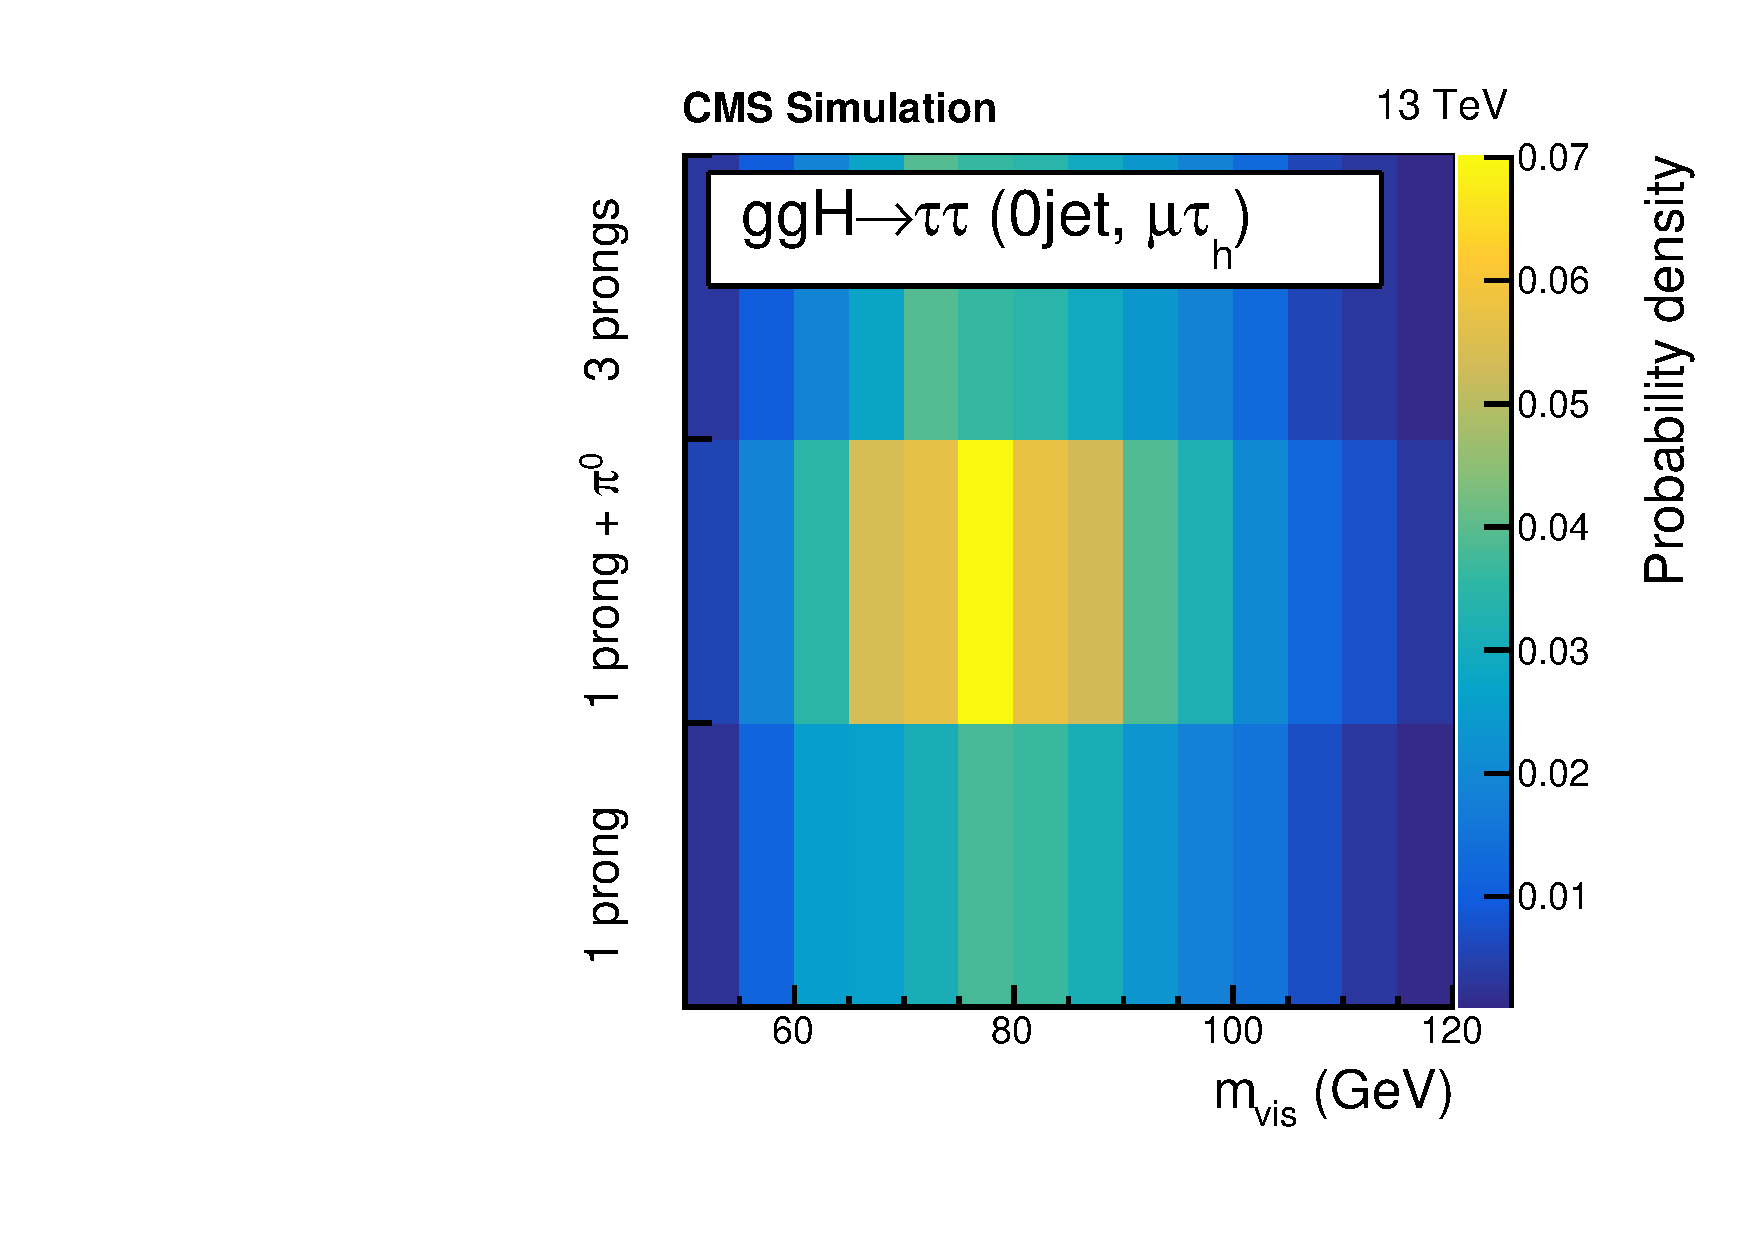
\includegraphics[width=0.4\textwidth]{higgs_to_taus/plots/Figure_001-a.pdf}
     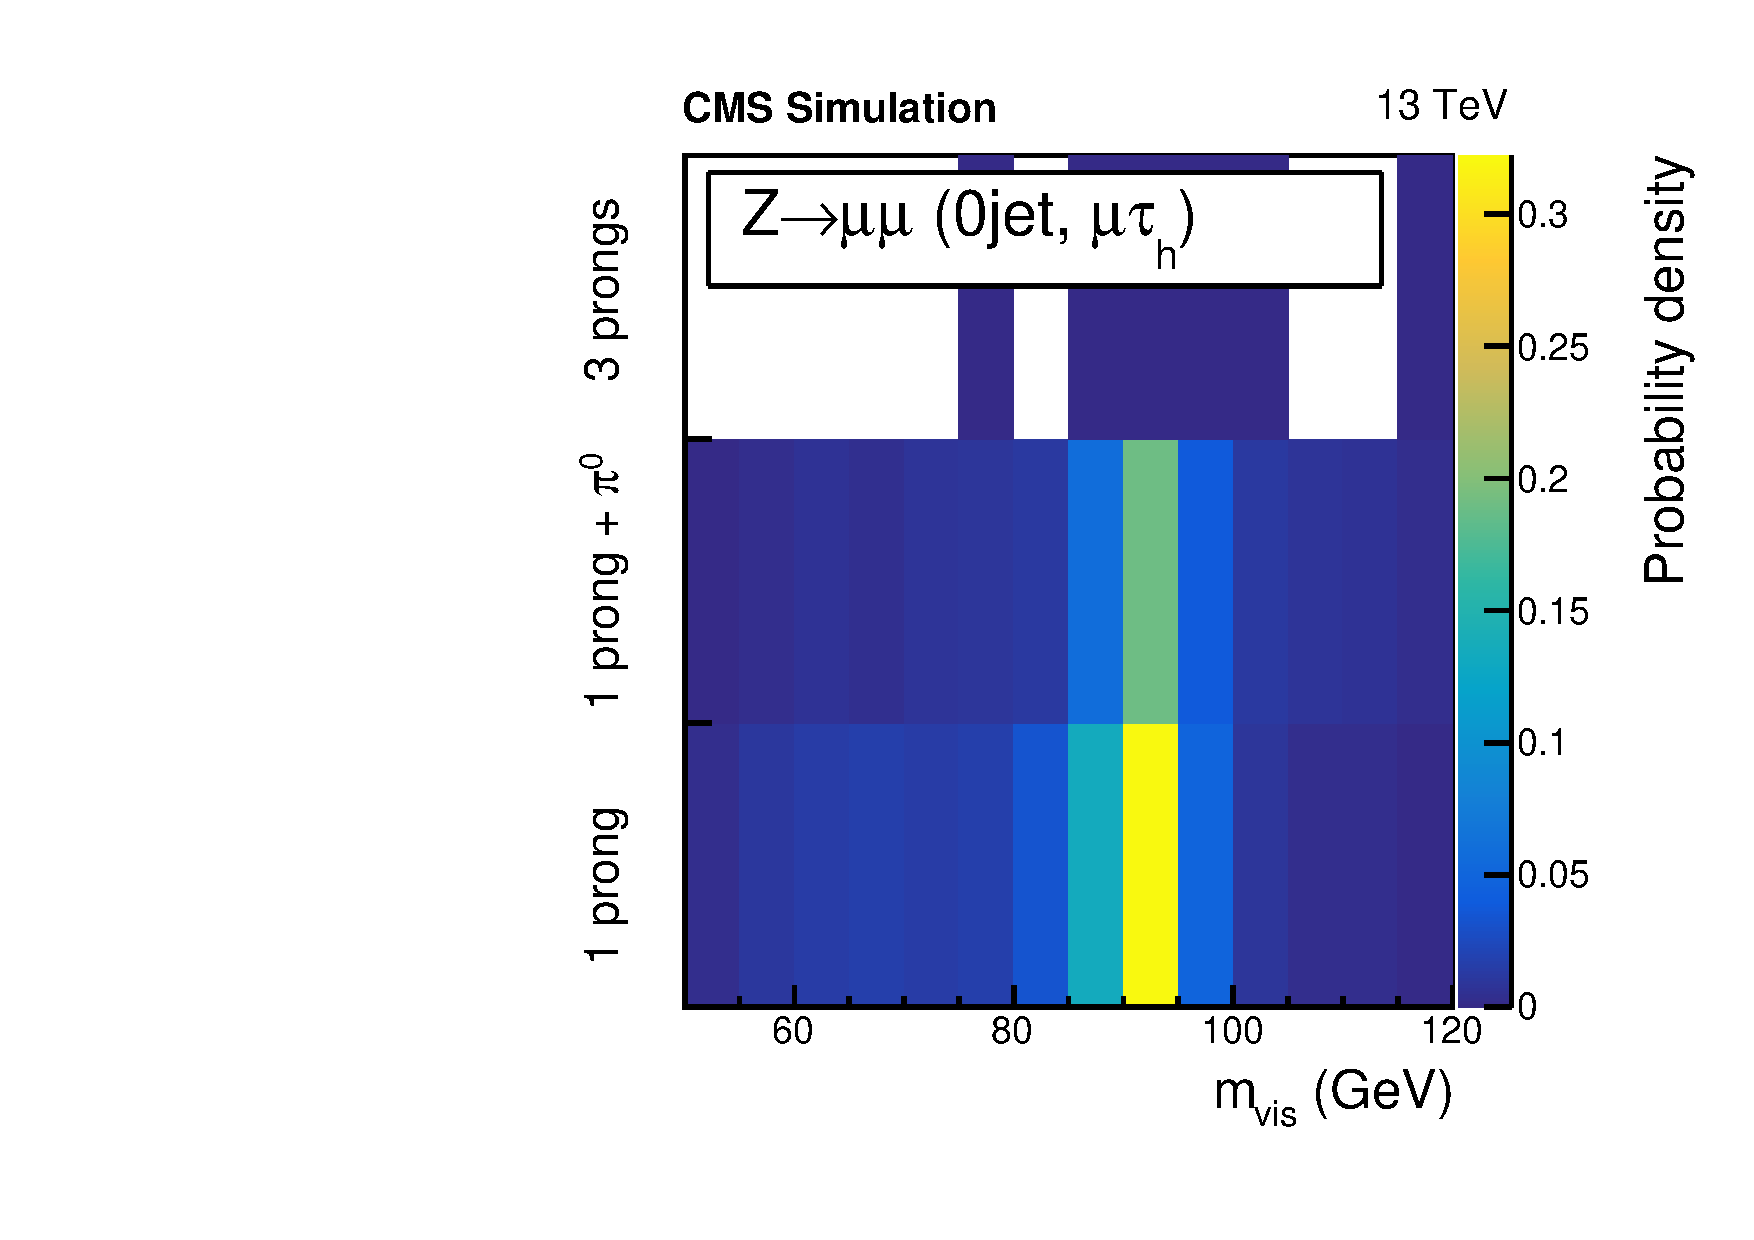
\includegraphics[width=0.4\textwidth]{higgs_to_taus/plots/Figure_001-b.pdf}\\
     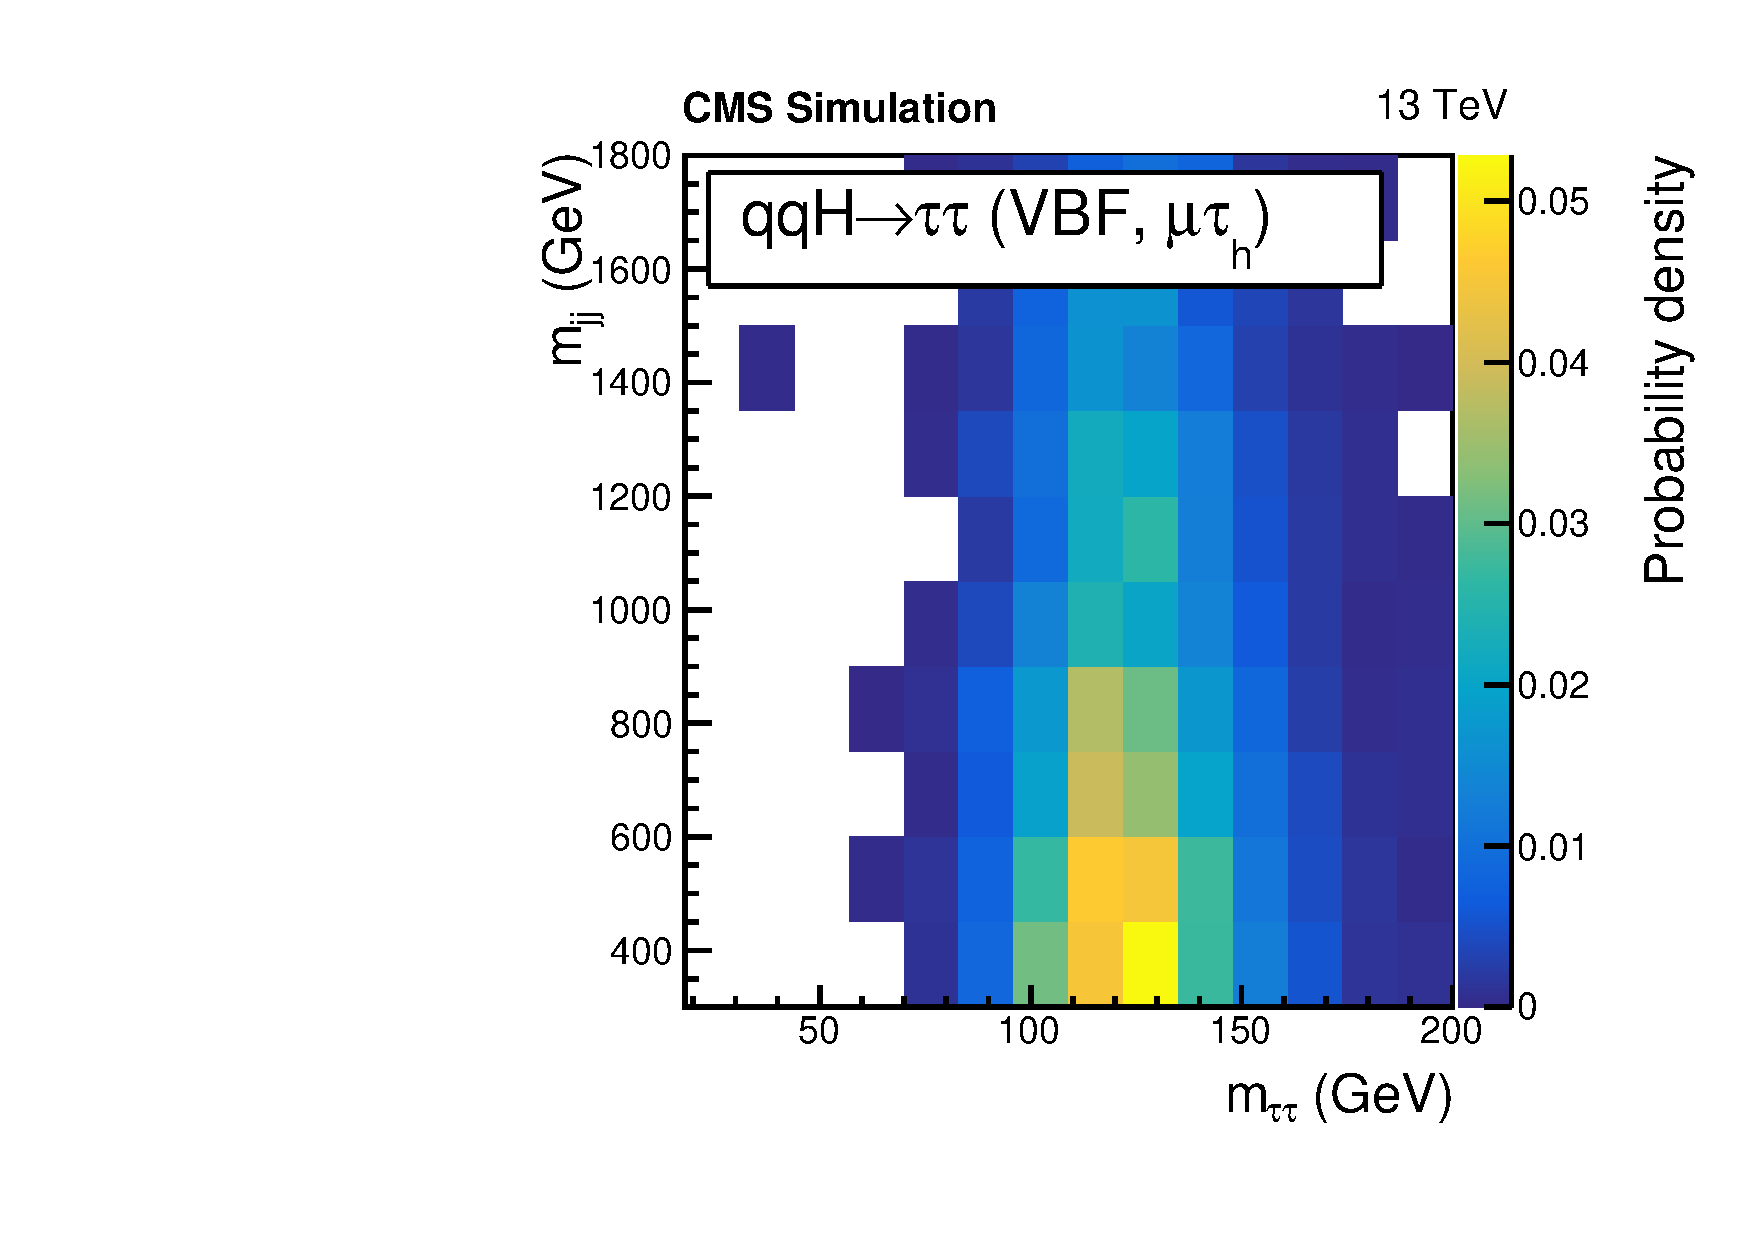
\includegraphics[width=0.4\textwidth]{higgs_to_taus/plots/Figure_001-c.pdf}
     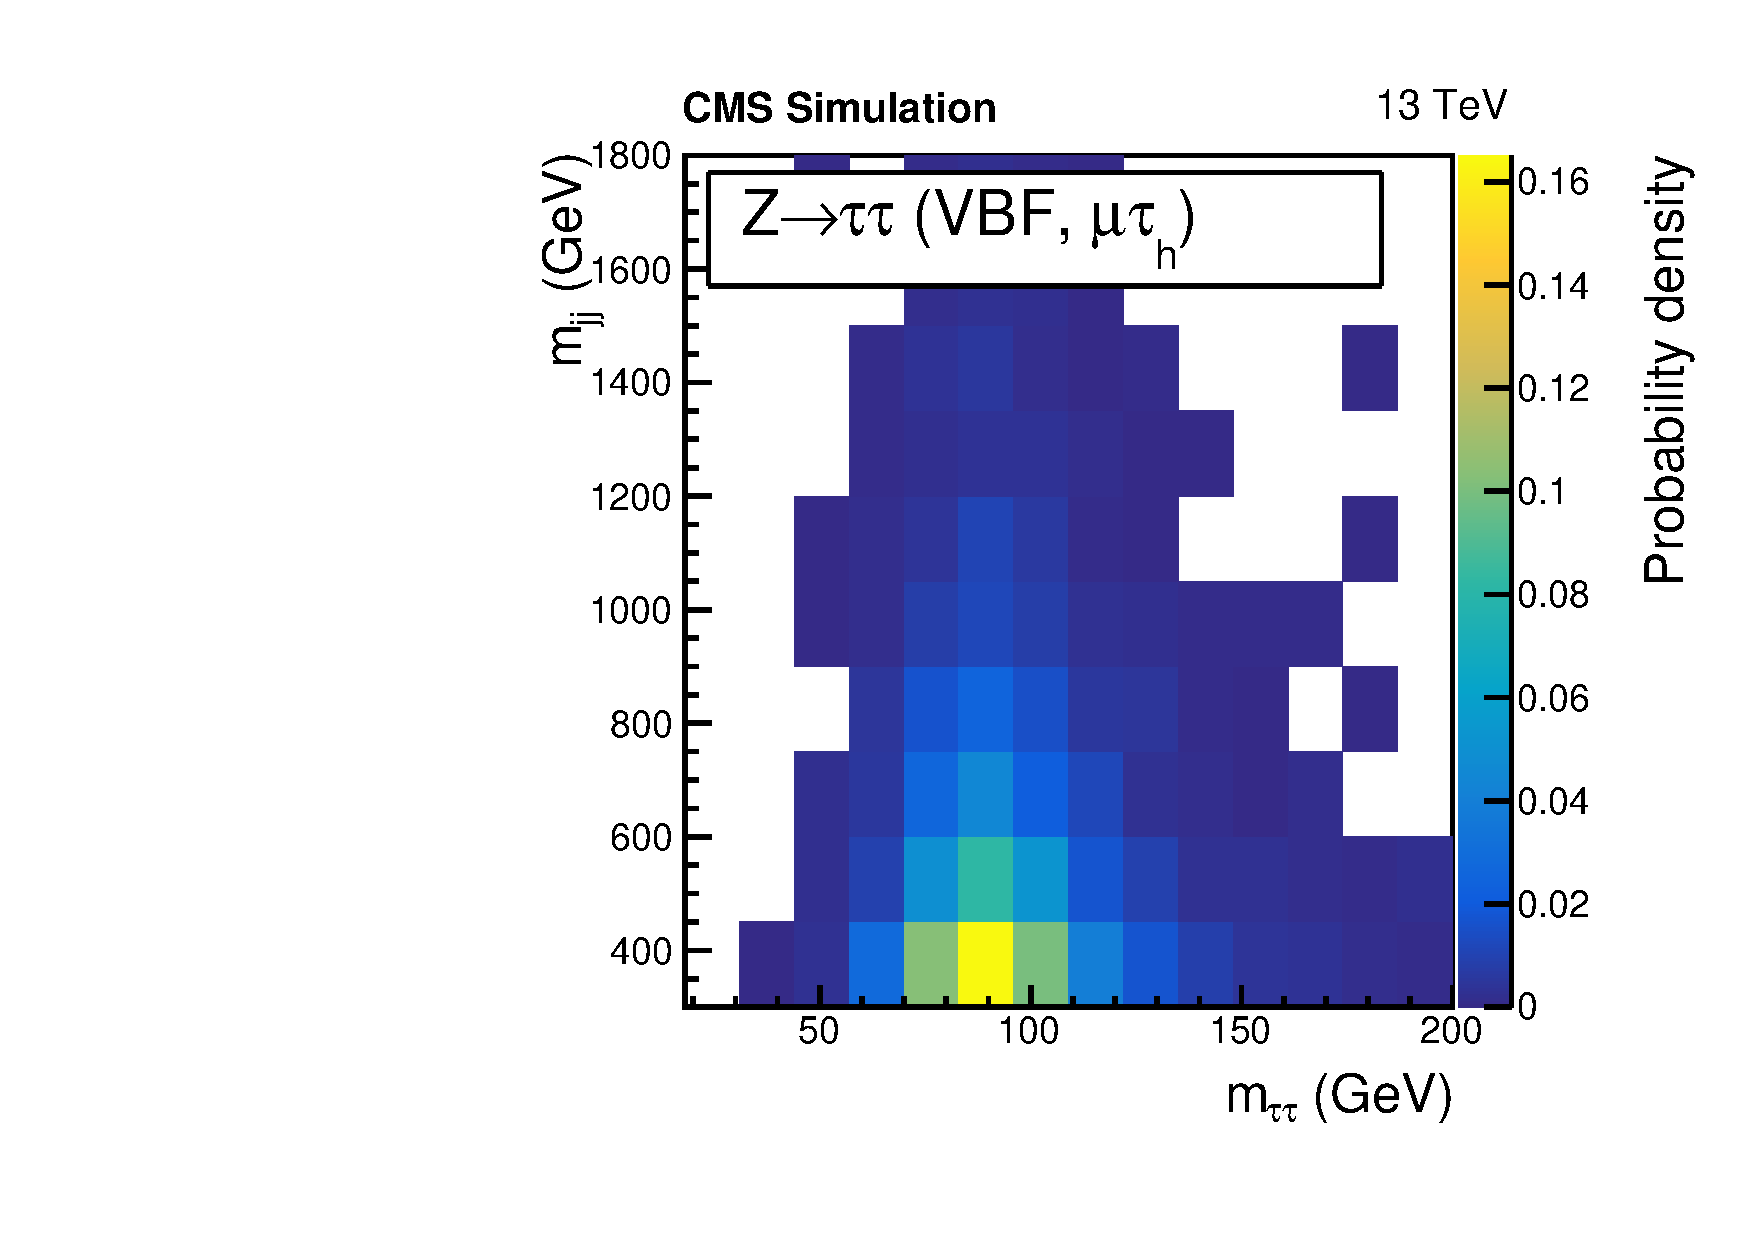
\includegraphics[width=0.4\textwidth]{higgs_to_taus/plots/Figure_001-d.pdf}\\
     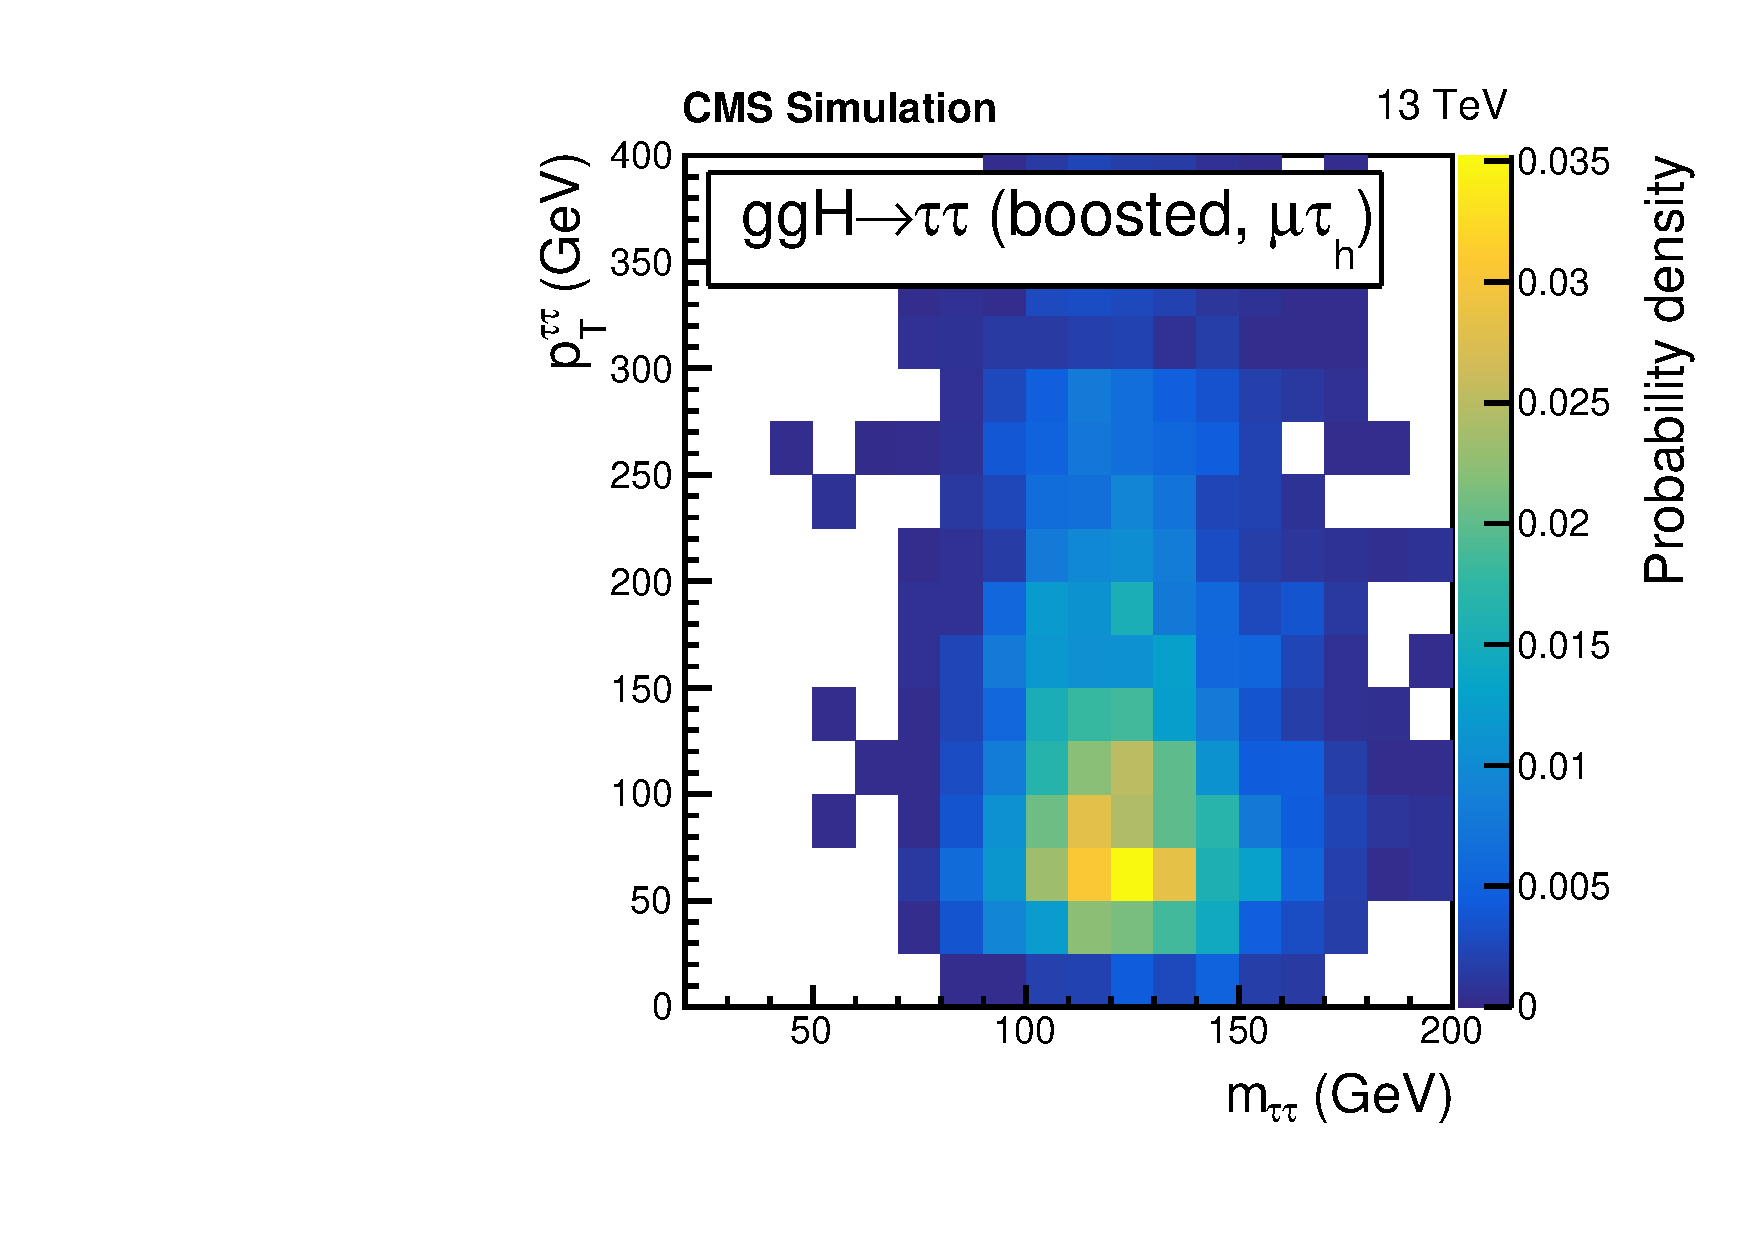
\includegraphics[width=0.4\textwidth]{higgs_to_taus/plots/Figure_001-e.pdf}
     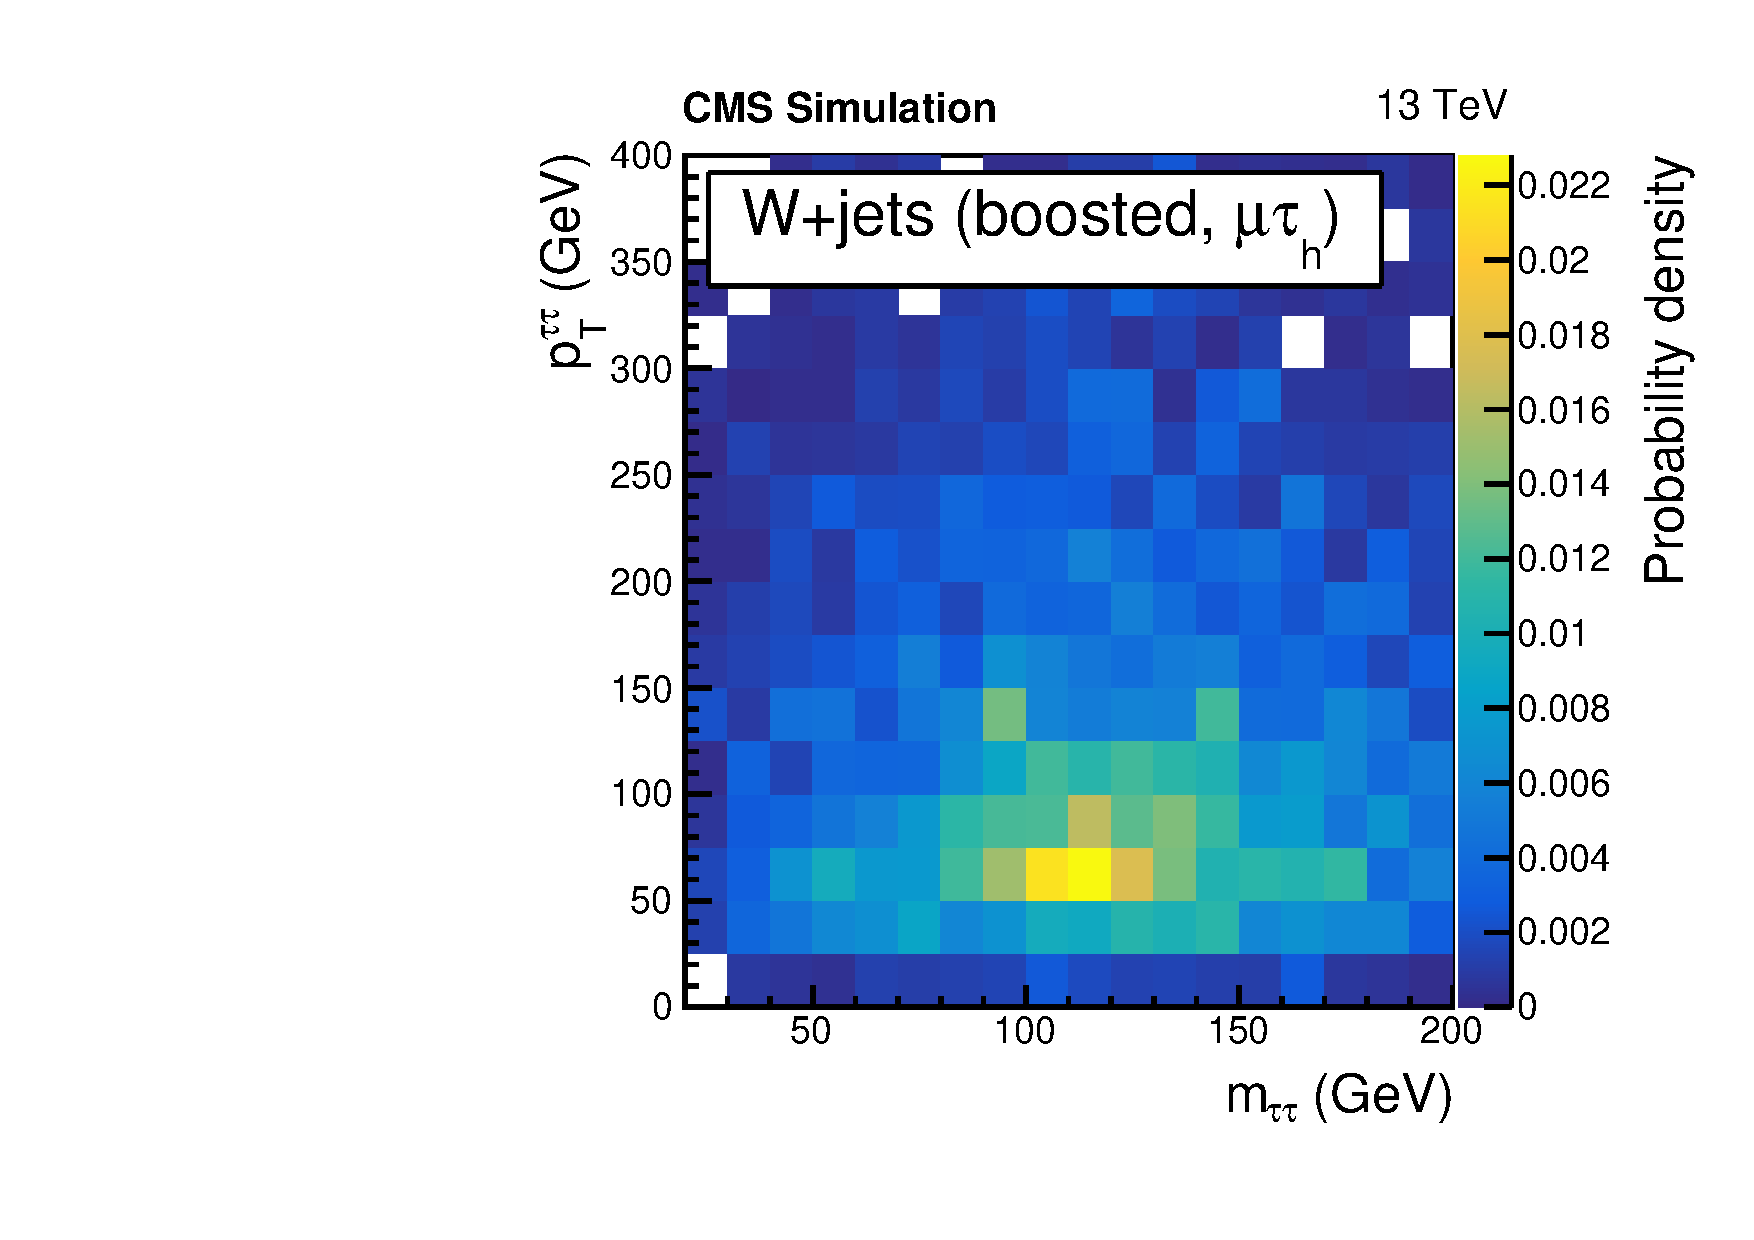
\includegraphics[width=0.4\textwidth]{higgs_to_taus/plots/Figure_001-f.pdf}
     \caption{Two dimensional unit normalized distributions for Higgs Boson events passing event selection 
for each category are shown (left). The specific Higgs Boson process shown is the one 
specifically targeted for each category. Distributions for select dominant background 
processes are shown (right). The rows correspond to the three categories: 0-jet (top), 
VBF (center), and boosted (bottom).  All distributions are from the $\Pgm\tauh$ decay channel.} 
\end{figure*}


\begin{table*}
\centering
\begin{small}
\begin{tabular}{llll}
 & 0-jet & VBF & Boosted \\
\hline
 & \multicolumn{3}{c}{Selection} \\ \cline{2-4}
$\tauh\tauh$ & No jet &  \scriptsize{$\geq$2 jets, $\pth>100\GeV$, $\Delta\eta_{\mathrm{jj}}>2.5$} & Others\\
$\Pgm\tauh$ & No jet &  \scriptsize{$\geq$2 jets, $\mjj>300\GeV$, $\pth>50\GeV$, $\pt^{\tauh}>40\GeV$} & Others\\
$\Pe\tauh$ & No jet &  \scriptsize{$\geq$2 jets, $\mjj>300\GeV$, $\pth>50\GeV$} & Others\\
$\Pe\Pgm$ & No jet & \scriptsize{2 jets, $\mjj>300\GeV$} & Others \\
\hline
 & \multicolumn{3}{c}{Observables}\\ \cline{2-4}
$\tauh\tauh$ & $\mtt$                 &    $\mjj$, $\mtt$  &   $\pth$, $\mtt$  \\
$\Pgm\tauh$ & $\tauh$ decay mode, $\mvis$   &    $\mjj$, $\mtt$  &  $\pth$, $\mtt$  \\
$\Pe\tauh$ & $\tauh$ decay mode, $\mvis$   &    $\mjj$, $\mtt$  &  $\pth$, $\mtt$ \\
$\Pe\Pgm$ & $\pt^{\Pgm}$, $\mvis$   &     $\mjj$, $\mtt$  &   $\pth$, $\mtt$  \\
\hline
\end{tabular}
\caption{ Category selection and observables used to build the 2D kinematic distributions. 
The events failing the 0-jet and VBF selection are included in the boosted category and are
denoted by ``Others''.
\label{tab:htt_categories}
}
\end{small}
\end{table*}

The results of the analysis are extracted with a global maximum likelihood fit based on  the 2D distributions in the various signal regions, and on some control regions, detailed in Section~\ref{sec:background_estimation}, that constrain the normalizations of the main backgrounds.

\section{Data Set}
The $\htt$ study utilizes the full 2016 $\pp$ dataset collected by CMS corresponding to 35.9$\fbinv$ 
of integrated luminosity.  The data were gathered at center-of-mass energy 13 TeV data from the LHC.
As data are gathered at CMS, the condition of the CMS detector are recorded simultaneously.
The CMS experiment uses an offline validation process to ensure that only high quality
data is used in future analyses.  Data collected while the CMS detector is in a faulty state
is flagged as such and, when an analyst processes the data, the faulty data is skipped.
When only considering the data considered good and usable for physics, the CMS experiment
gathered 35.9$\fbinv$ of integrated lumiosity.

In this analysis only a subset of the total data marked as good is used.  During data
gathering, data is filtered into primary datasets (PDs) corresponding to which HLT trigger
made the determination to save a given event.  The HLT triggers using in this analysis,
detailed in table~\ref{tab:htt_hlt_triggers}, correspond to: the Single Electron/Photon
PD, the Single Muon PD, the Muon and Electron PD, and the Tau PD.



\section{Monte Carlo Samples}
Signal and background processes are modeled with samples of simulated events.
For details on the production for simulated events, see section~\ref{sec:simulation}.

The signal samples with a Higgs Boson produced vai the gluon fusion production
mechanism ($\cPg\cPg\PH$), vector boson fusion (VBF), or in association with a $\PW$ or $\PZ$ boson ($\PW\PH$ or $\PZ\PH$), 
are generated at next-to-leading order (NLO) in perturbative quantum chromodynamics (pQCD) 
with the \POWHEG 2.0~\cite{Nason:2004rx,Frixione:2007vw, Alioli:2010xd, Alioli:2010xa, Alioli:2008tz} 
generator. For the $\PW\PH$ and $\PZ\PH$ simulated samples, the \textsc{minlo hvJ}~\cite{Luisoni:2013kna} 
extension of \POWHEG 2.0 is used. The set of parton distribution functions (PDFs) used for all
simulates samples is NNPDF30\_nlo\_as\_0118~\cite{Ball:2011uy}. It is found that the $\ttbar\PH$ 
process is negligible in comparison with the other signal processes and is therefor excluded.
Mass dependant production cross sections and $\htt$ branching fractions for the SM Higgs Boson production, 
and their corresponding uncertainties are taken from 
Refs.~\cite{deFlorian:2016spz,Denner:2011mq,Ball:2011mu} and references therein.

The $\text{MG5}_\aMCATNLO$~\cite{Alwall:2014hca} generator is used for $\PZ+$jets and $\PW+$jets processes. 
They are simulated at leading order (LO) with MLM jet matching and merging~\cite{Alwall:2007fs}.
The \aMCATNLO generator is also used for diboson production simulated at next-to-LO (NLO) with the 
FxFx jet matching and merging~\cite{Frederix:2012ps}. In contrast, \POWHEG 2.0 and 1.0 are used for \ttbar
and single top quark production, respectively. The generators are interfaced with \PYTHIA 
8.212 ~\cite{Sjostrand:2014zea} to model the parton showering and fragmentation, as well as 
the decay of the $\Pgt$ leptons. The \PYTHIA parameters affecting the description of the 
underlying event are set to the {CUETP8M1} tune~\cite{Khachatryan:2015pea}.

A event-by-event weight is applied to the simulated events such that the distribution of the 
number of additional pileup interactions in the simulated sample more closely aligns with that in data.
The distribution of additional pileup interactions in data is estimated from the measured instantaneous 
luminosity for each bunch crossing. The average number of additional pileup interactions in
data is approximately 27 interactions per bunch crossing.



\section{SVFit Algorithm}



\section{Background Estimation}
The largest irreducible source of background is the Drell--Yan production
of $\PZ/\Pgg^*\to\Pgt\Pgt, \ell\ell$. Proper shape and normalization for this
leading background is critical is critical to the success of the analysis.
A dedicated, high purity, $\PZ/\Pgg^*\to\Pgm\Pgm$ control region was
used to measure reweighting factors for application to all Drell--Yan
simulated events and is detailed in the Monte Carlo Corrections 
section~\ref{sec:mc_corrections}.

The $\PW+\text{jets}$ process is modelled using simulation.
In the $\tauh\tauh$ and $\Pe\Pgm$ channels the $\PW+\text{jets}$ contribution 
is small compared to other backgrounds. In these two channels both the shape and 
yield are taken from simulation.
The background from $\PW+\text{jets}$ production contributes significantly to the
$\Pgm\tauh$ and $\Pe\tauh$ channels, when the $\PW$ boson decays leptonically and
a jet is misidentified as a $\tauh$ candidate. In the $\ell\tauh$ channels
the shape of the background is simulation based while the yields are estimated 
using data in a $\PW+\text{jets}$ enriched dedicated side-band region defined
based on transverse mass, $\MT > 80\GeV$. In this high-$\MT$ side-band region, the $\PW+\text{jets}$
process is scaled so that the sum total of expected background events is equivalent
to the sum total of observed data events. The scaling factor is then applied
in the low transverse mass signale regions $\MT < 50\GeV$. A scaling factor
is measured for the 0-jet and Boosted categories for both $\Pe\Pgt$ and $\Pgm\Pgt$ resulting
in four $\PW+\text{jets}$ scaling values. The scaling factor measured in the Boosted
category is extrapolated to the VBF category. The $\PW+\text{jets}$ purity in these
side-band regions varies from about 50\% in the boosted category to 85\% in the 0-jet category.

The high-$\MT$ side-bands, described above, are included as a control regions in the final fit.
These high-$\MT$ $\PW+\text{jets}$ control regions can be seed in Figure~\ref{fig:htt_wj_CR1}.
The control regions are only a singular bin because they are used solely to constrain 
the normalization of the $\PW+\text{jets}$ process.

\begin{figure*}[!htbp]
\centering
     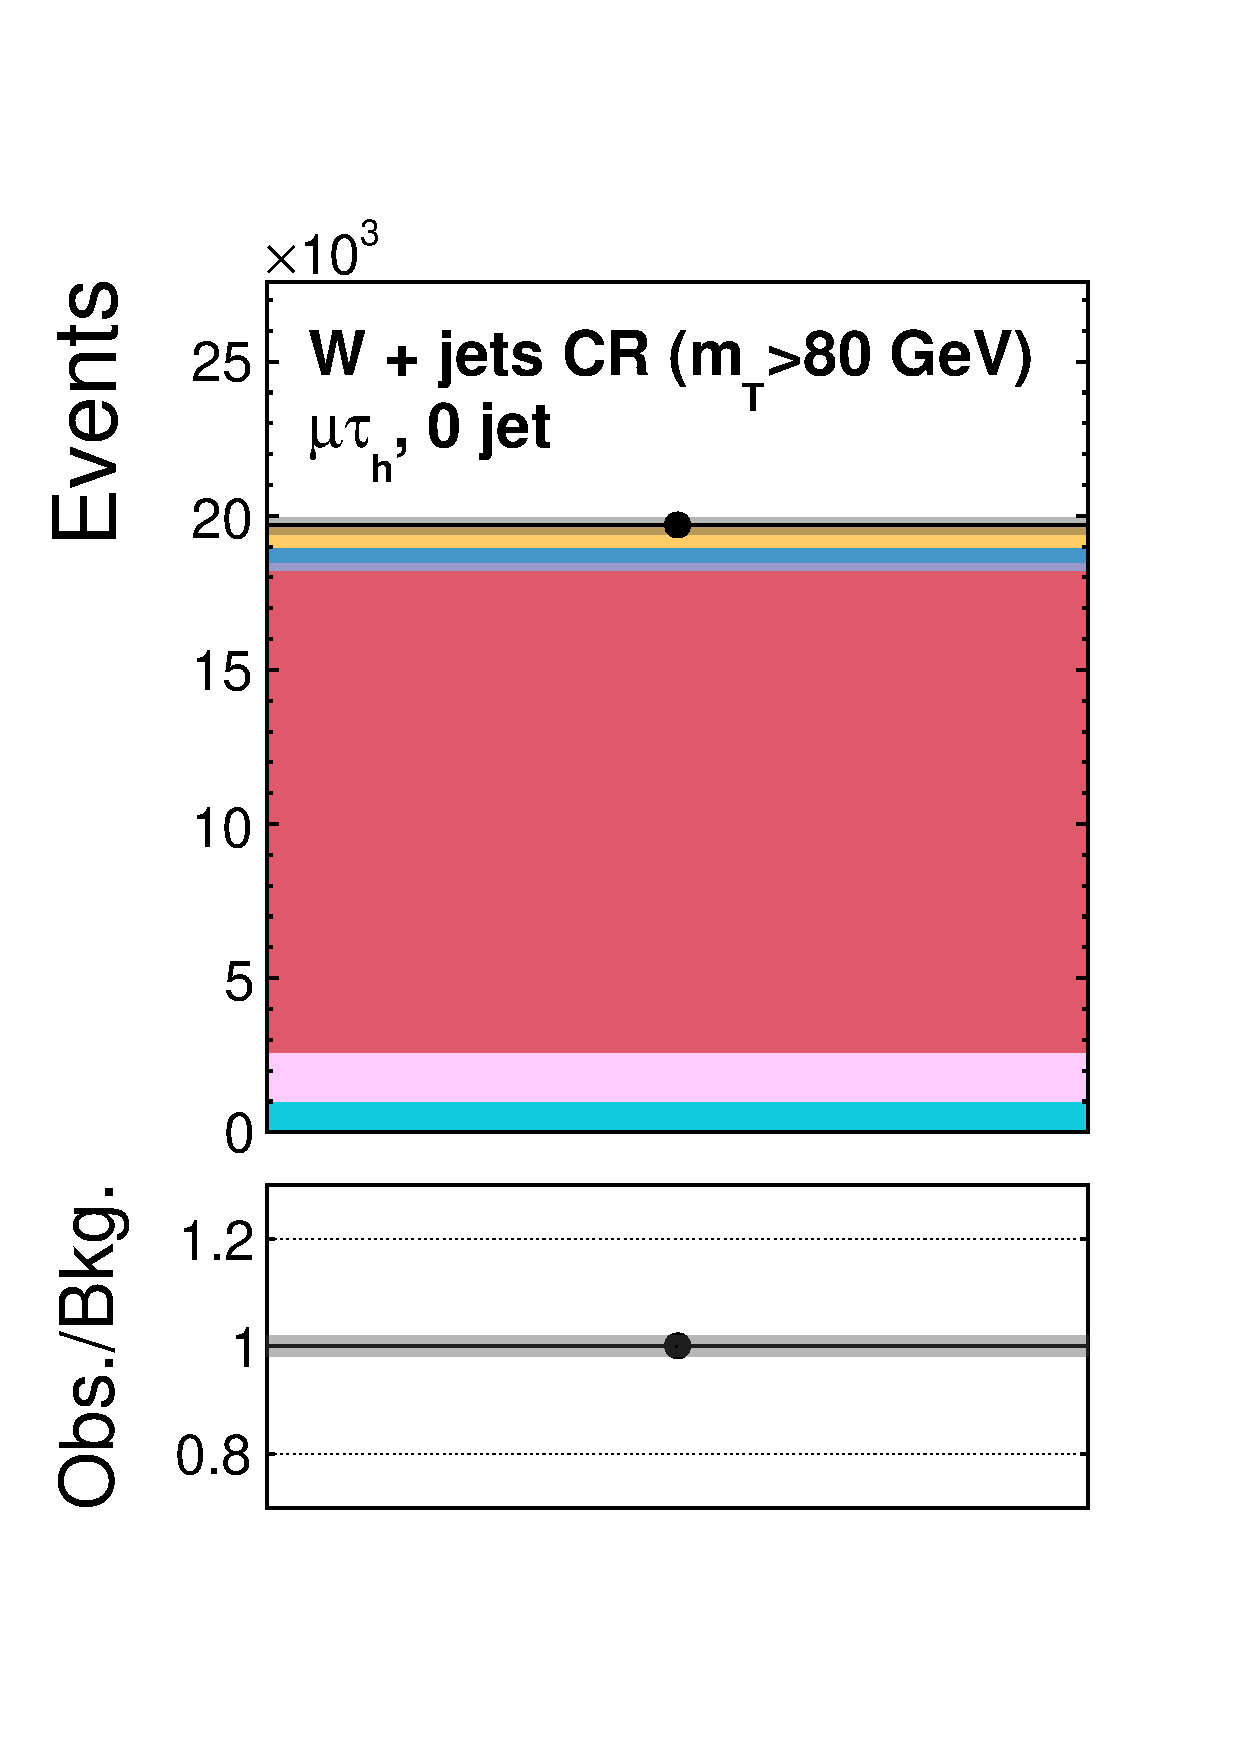
\includegraphics[width=0.19\textwidth]{higgs_to_taus/plots/Figure_002-a.pdf}
     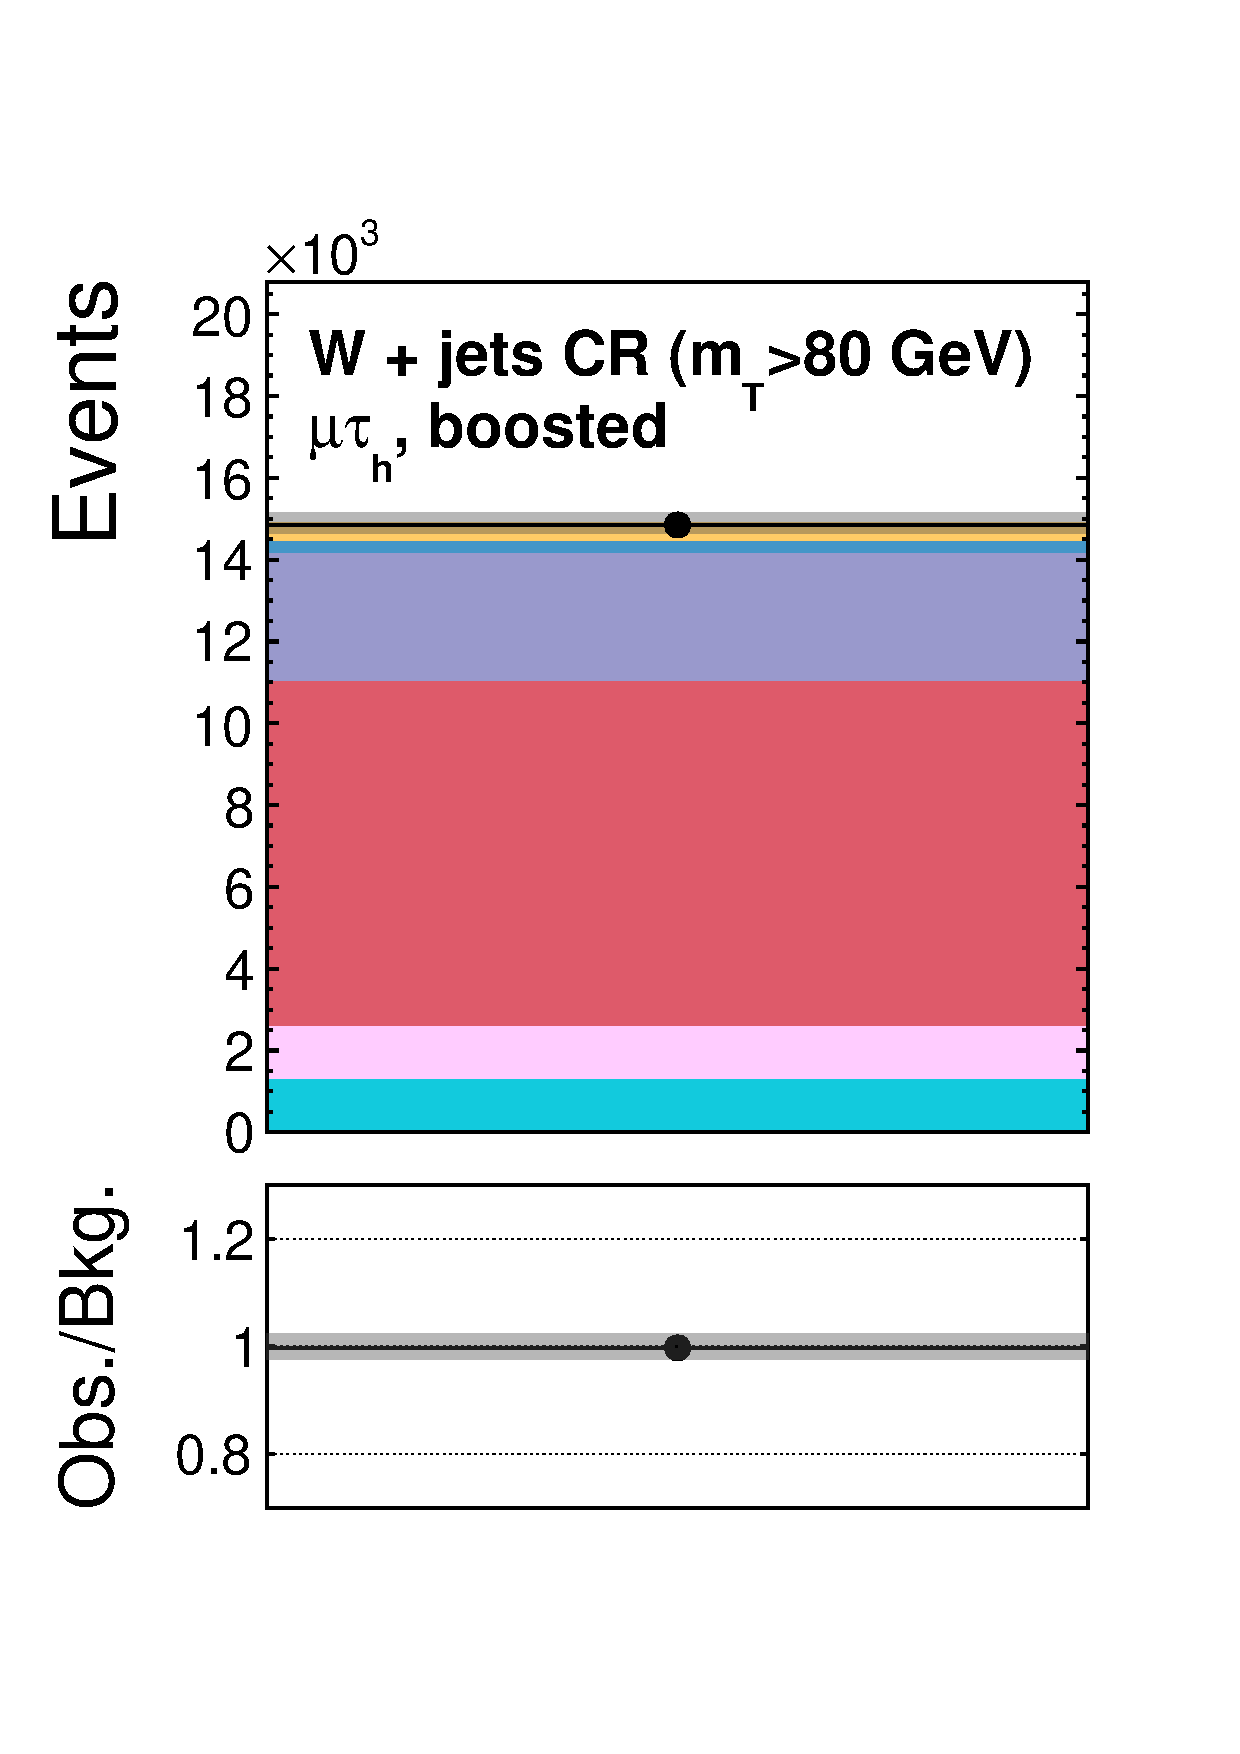
\includegraphics[width=0.19\textwidth]{higgs_to_taus/plots/Figure_002-b.pdf}
     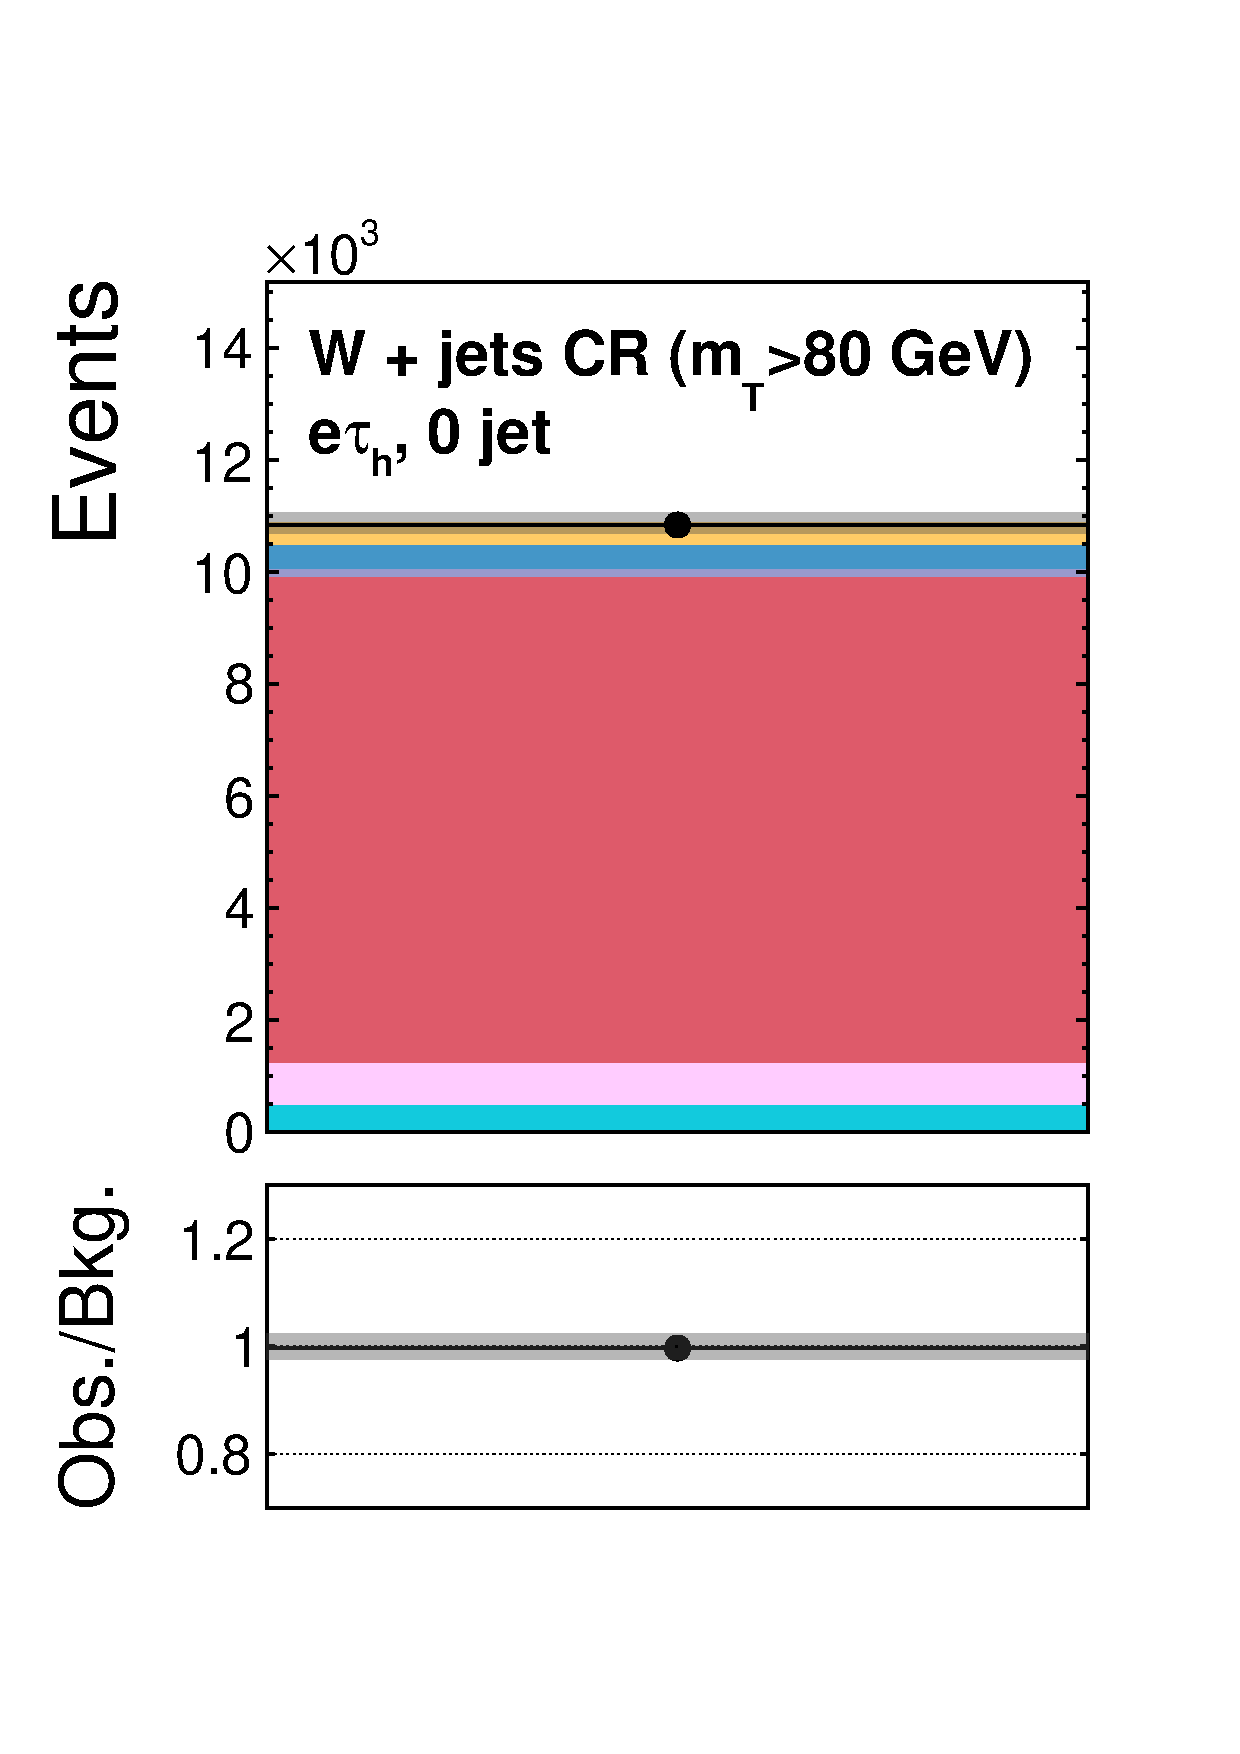
\includegraphics[width=0.19\textwidth]{higgs_to_taus/plots/Figure_002-c.pdf}
     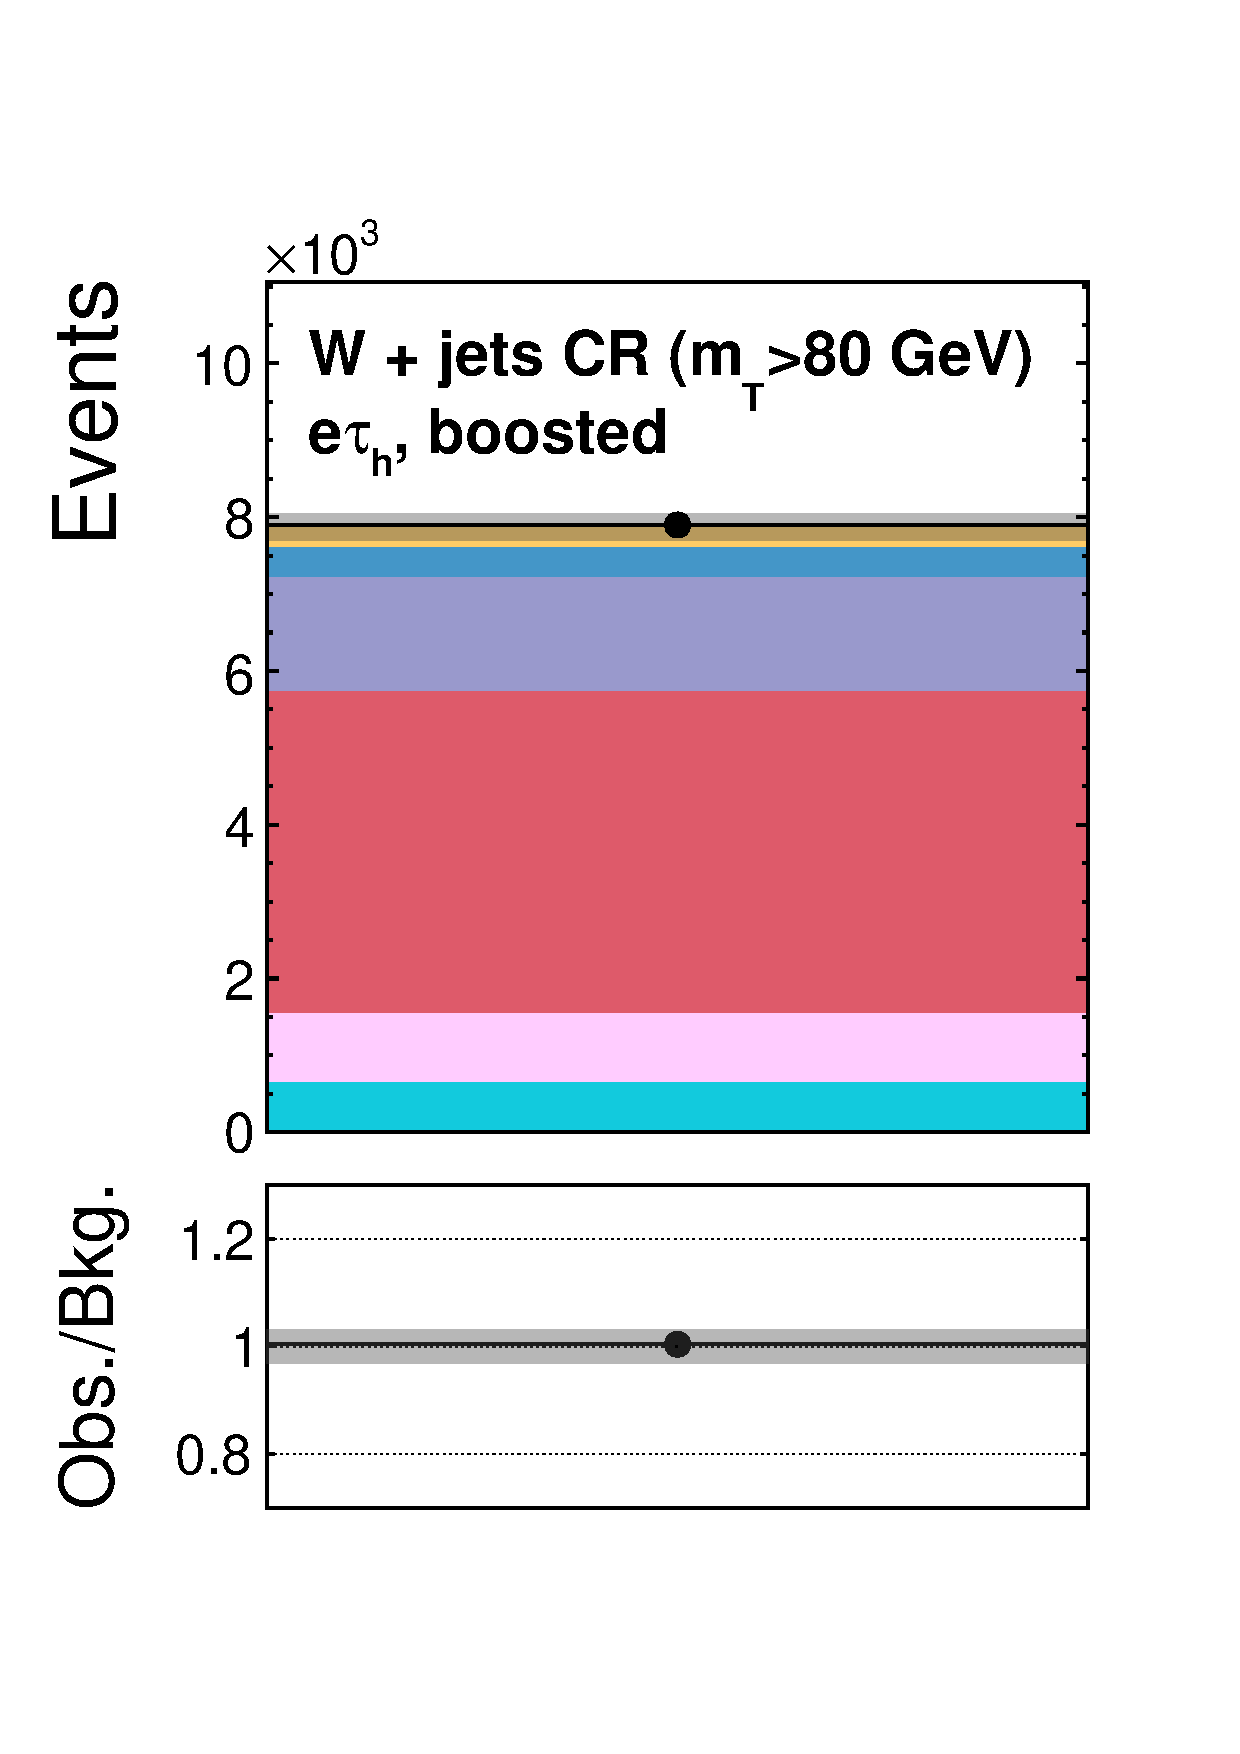
\includegraphics[width=0.19\textwidth]{higgs_to_taus/plots/Figure_002-d.pdf}
     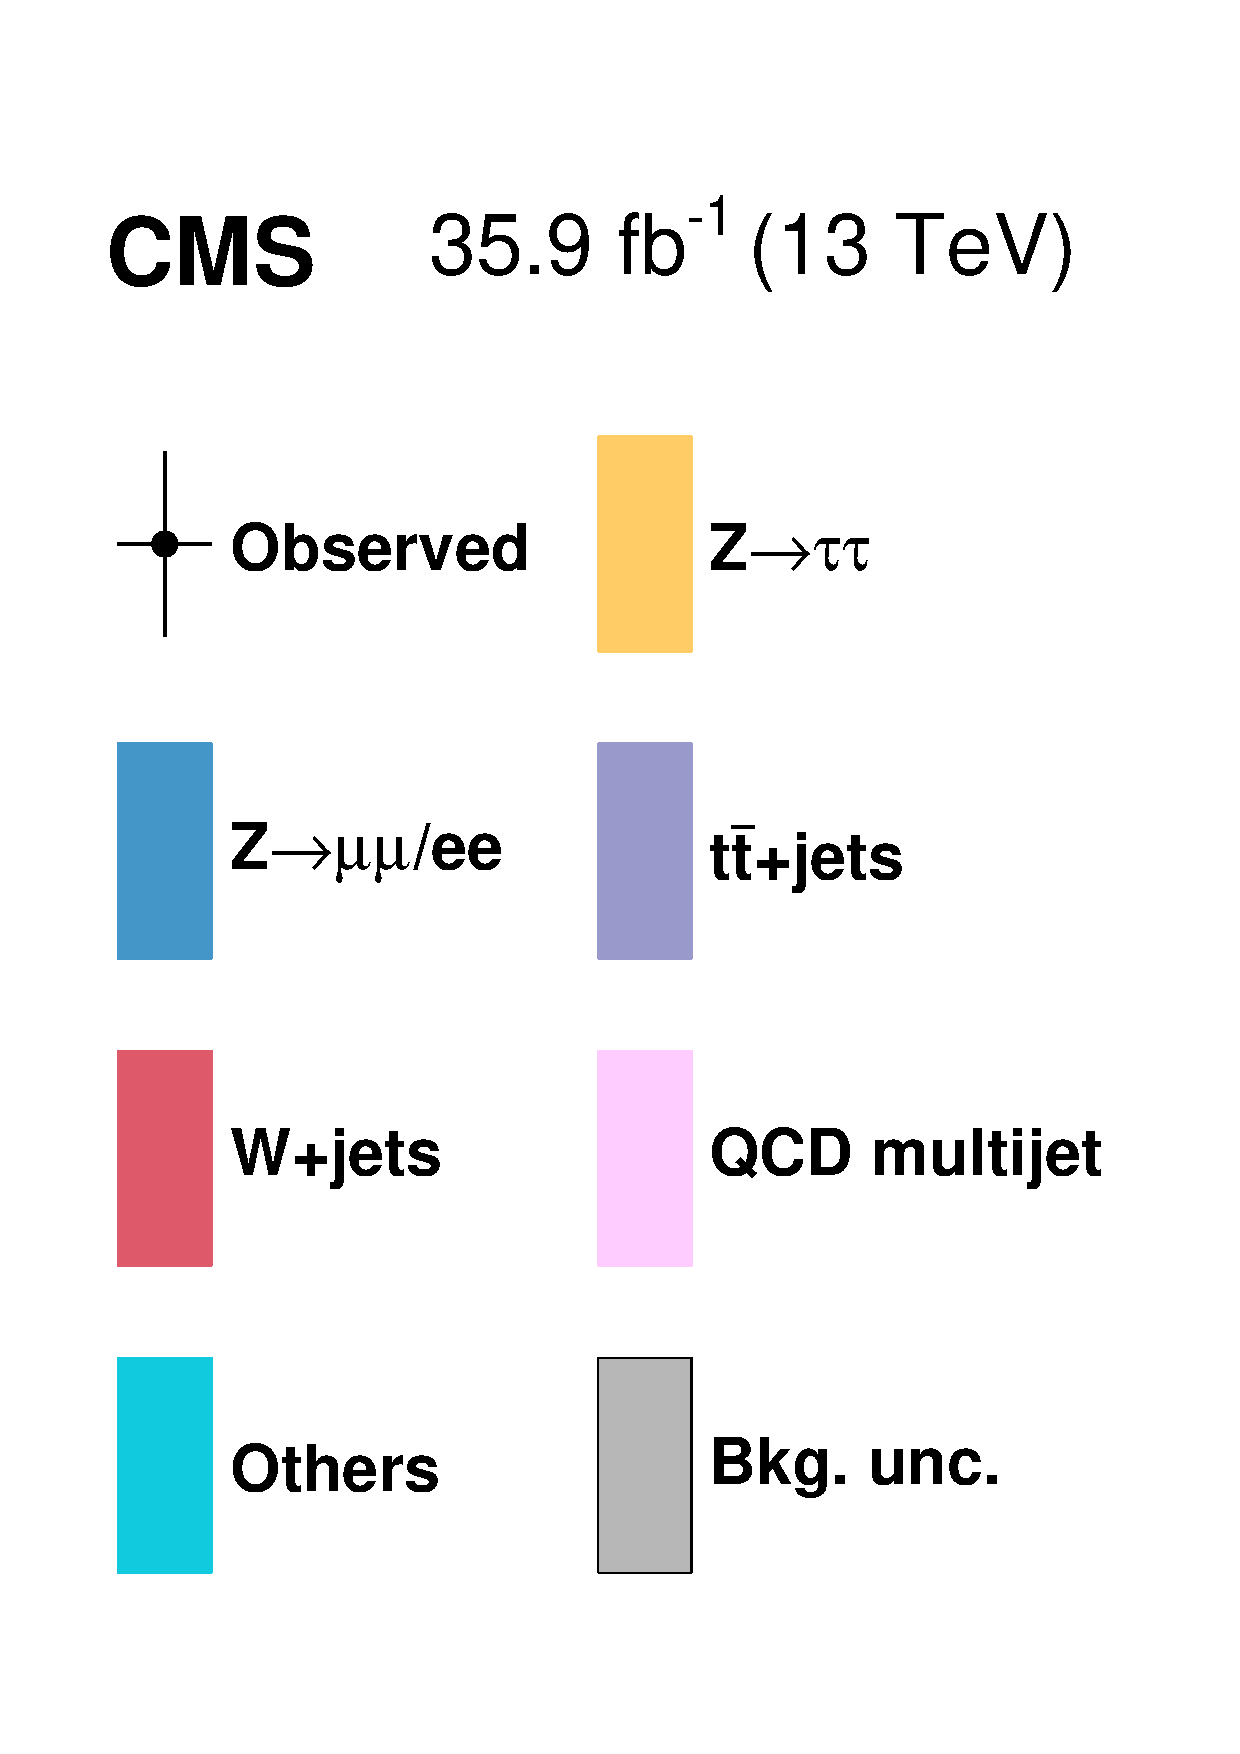
\includegraphics[width=0.19\textwidth]{higgs_to_taus/plots/Figure_002-e.pdf}
     \caption{the high-$\MT$ control regions enriched in the $\PW+\text{jets}$ background used in 
the maximum likelihood fit, together with the signal regions, to extract the results. 
The normalization of the predicted background distributions corresponds to the result of 
the global fit. These regions, defined with $\MT>80$\GeV, control the yields of the 
$\PW+\text{jets}$ background in the $\Pgm\tauh$ and $\Pe\tauh$ channels.  
The constraints obtained in the boosted categories are propagated to the VBF categories 
of the corresponding channels.}
     \label{fig:htt_wj_CR1}
\end{figure*}


The QCD multijet process constitutes an important source of reducible background 
in the $\tauh\tauh$ and $\ell\tauh$ channels. The QCD multijet process is subdominant
in the $\Pe\Pgm$ channel. For all four channels, the QCD multijet, is entirely estimated from data.  
Side-band control regions are constructed to estimate the shape and the yield of the QCD multijet 
background in these channels.

QCD multijet estimation for the $\ell\tauh$ channels follows:
\begin{enumerate}

\item Raw yield is extracted using a sample where the
$\ell$ and the $\tauh$ candidates have the same-sign charge. Using this sample, the QCD multijet 
process is estimated from data by subtracting the contribution of the Drell--Yan, \ttbar, diboson,
and $\PW+\text{jets}$ processes as in equation~\ref{eqn:qcd_eqn}. The $\PW+\text{jets}$ processes has been scaled by the
$\PW+\text{jets}$ high-$\MT$ to low-$\MT$ scale factor described previously.
\begin{equation}
\label{eqn:qcd_eqn}
\text{QCD} = \text{Data} - \text{Other Background Processes}
\end{equation}

\item The raw yield obtained above is corrected to account for observed differences between the background 
composition in the same-sign and opposite-sign regions. The extrapolation factor between the same-sign 
and opposite-sign regions is determined by comparing the yield of the estimated QCD multijet background for 
events with $\ell$ candidates passing inverted isolation criteria, in the same-sign and opposite-sign 
regions. It is constrained and measured by adding to the global fit the opposite-sign region where 
the $\ell$ candidates pass inverted isolation criteria, using the QCD multijet background estimate 
from the same-sign region with $\ell$ candidates passing inverted isolation criteria. For the same 
reasons as in the case of the W+jets background, the constraints are also extrapolated to the VBF 
signal region. 
%Figure~\ref{fig:htt_qcd_CR3} shows these control regions for the 0-jet and boosted categories 
%of the $\Pgm\tauh$ and $\Pe\tauh$ channels; the observable is $\mvis$ or $\mtt$ to provide 
%discrimination between the QCD multijet and the $\PZ\to\Pgt\Pgt$ processes.

\item The 2D distributions of the QCD multijet background are estimated from a region with 
same-sign leptons, same as the yield estimate, except the isolation of the $\ell$ and $\tauh$ 
candidates is additionally relaxed to reduce the statistical fluctuations in the distributions. 
The contributions from other background process are subtracted from data, eqn.~\ref{eqn:qcd_eqn},
to extract the QCD multijet shape template in this region.
\end{enumerate}

The same technique is used in the $\Pe\Pgm$ channel, except no control region is included in the 
fit because QCD multijet events contribute little to the total background in this decay channel.

%\begin{figure*}[!htbp]
%\centering
%     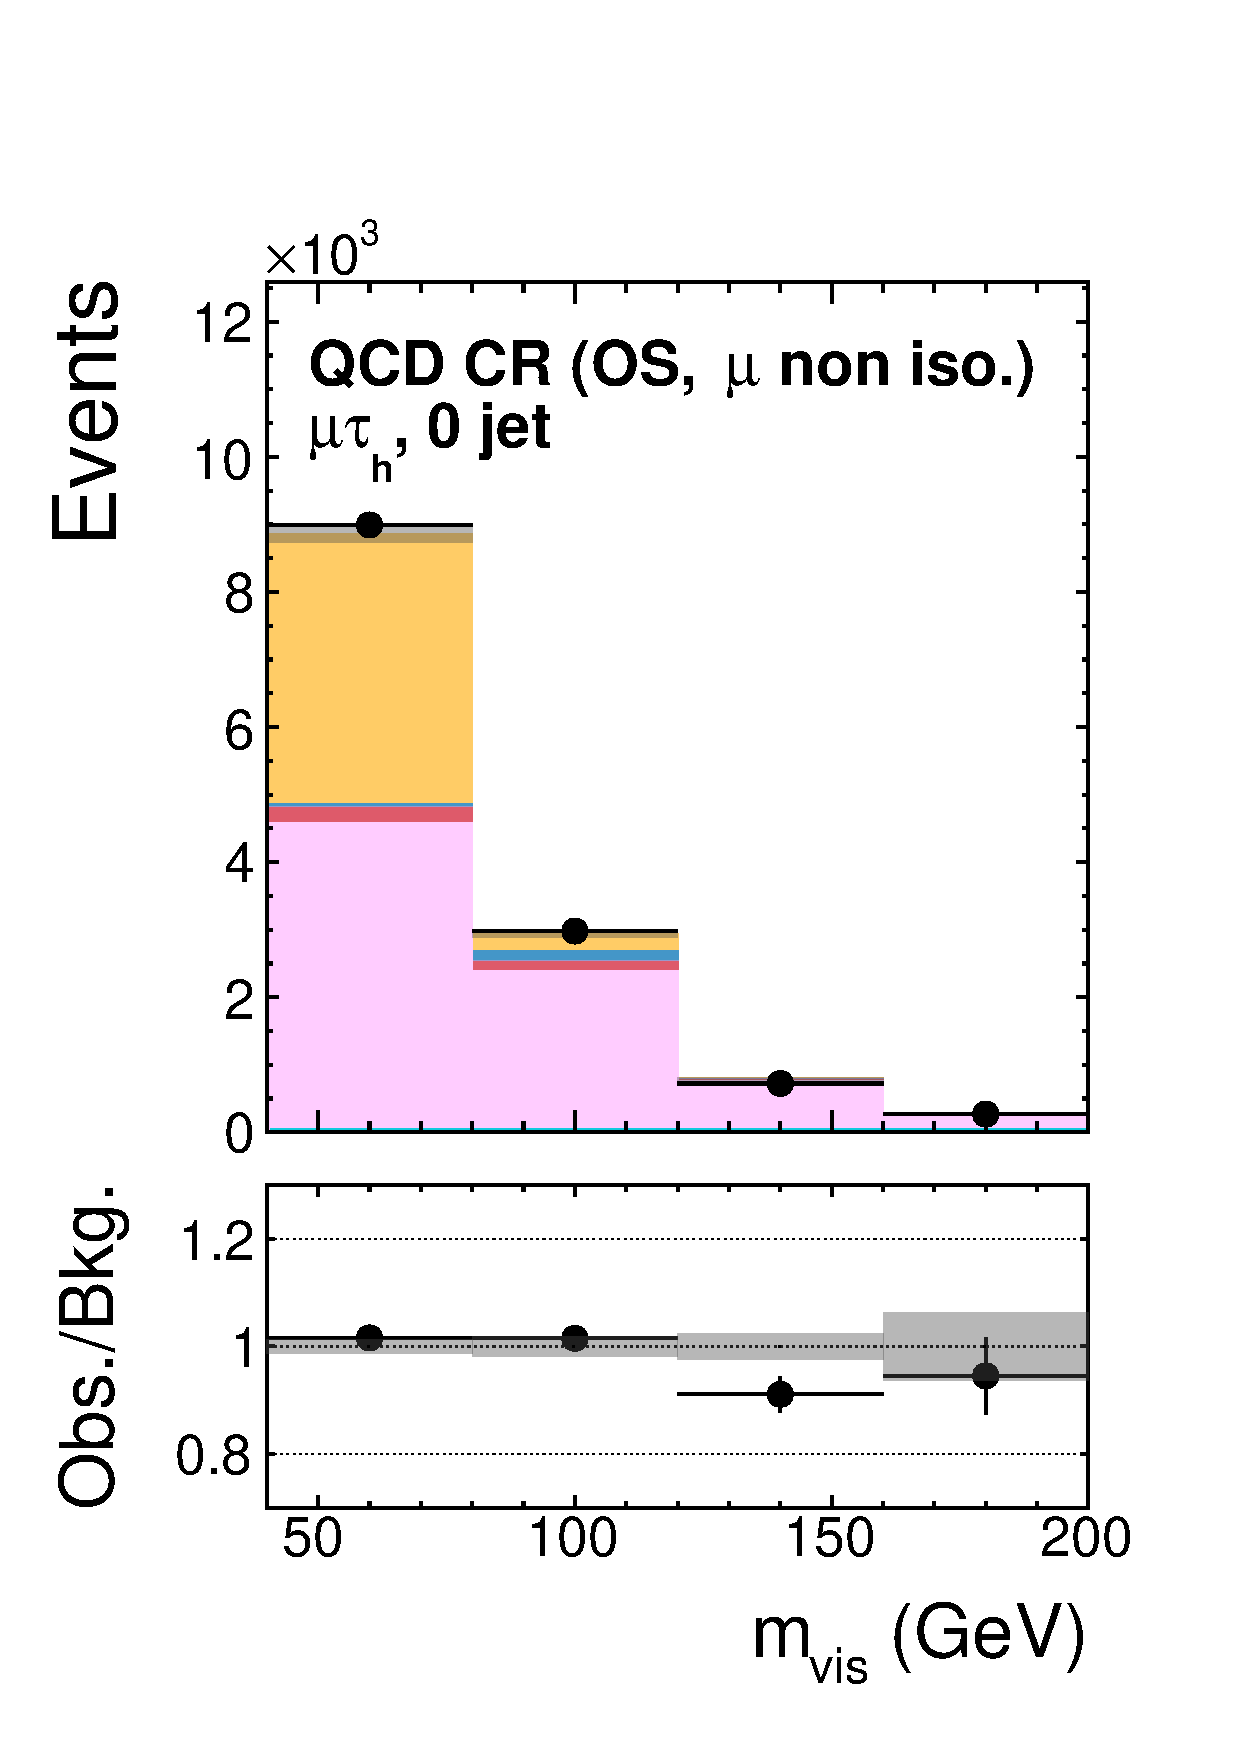
\includegraphics[width=0.3\textwidth]{higgs_to_taus/plots/Figure_003-a.pdf}
%     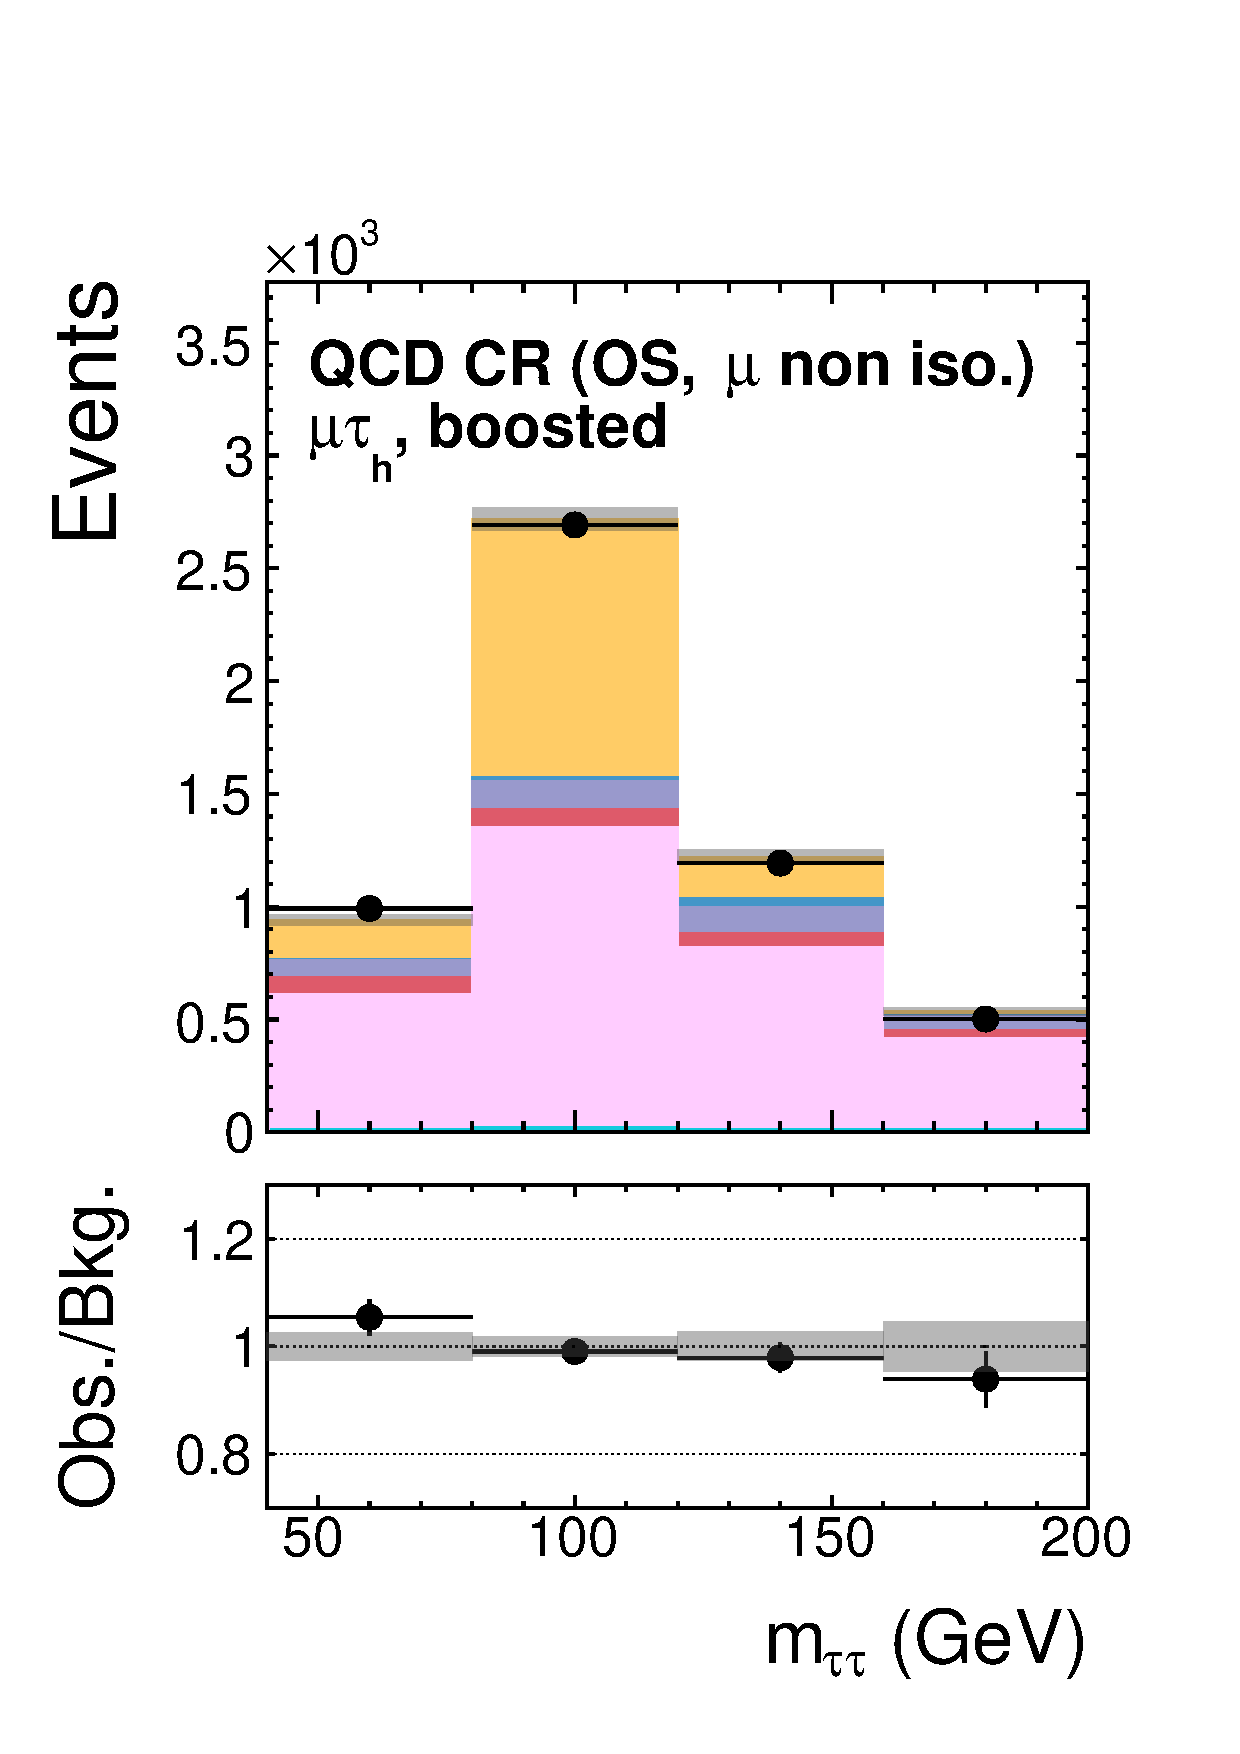
\includegraphics[width=0.3\textwidth]{higgs_to_taus/plots/Figure_003-b.pdf}
%     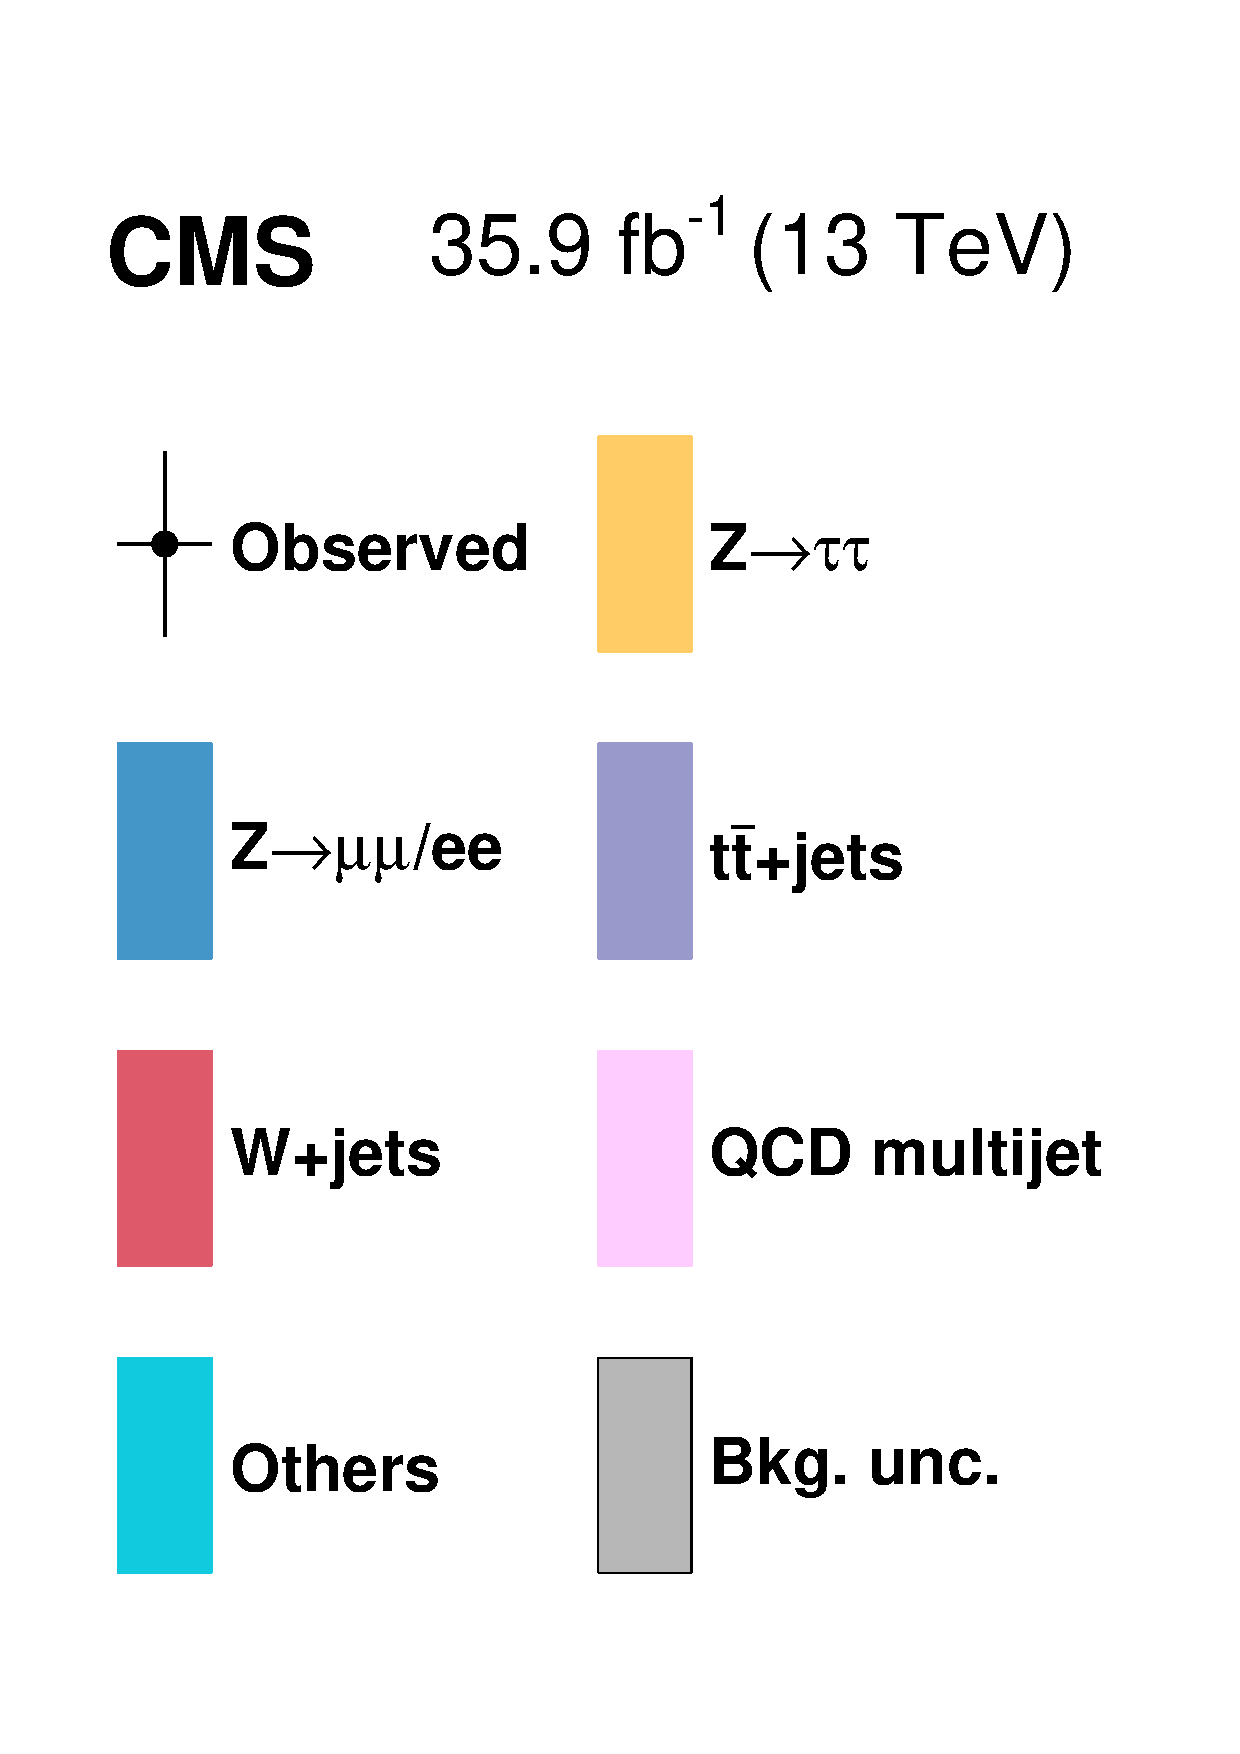
\includegraphics[width=0.3\textwidth]{higgs_to_taus/plots/Figure_003-c.pdf}
%     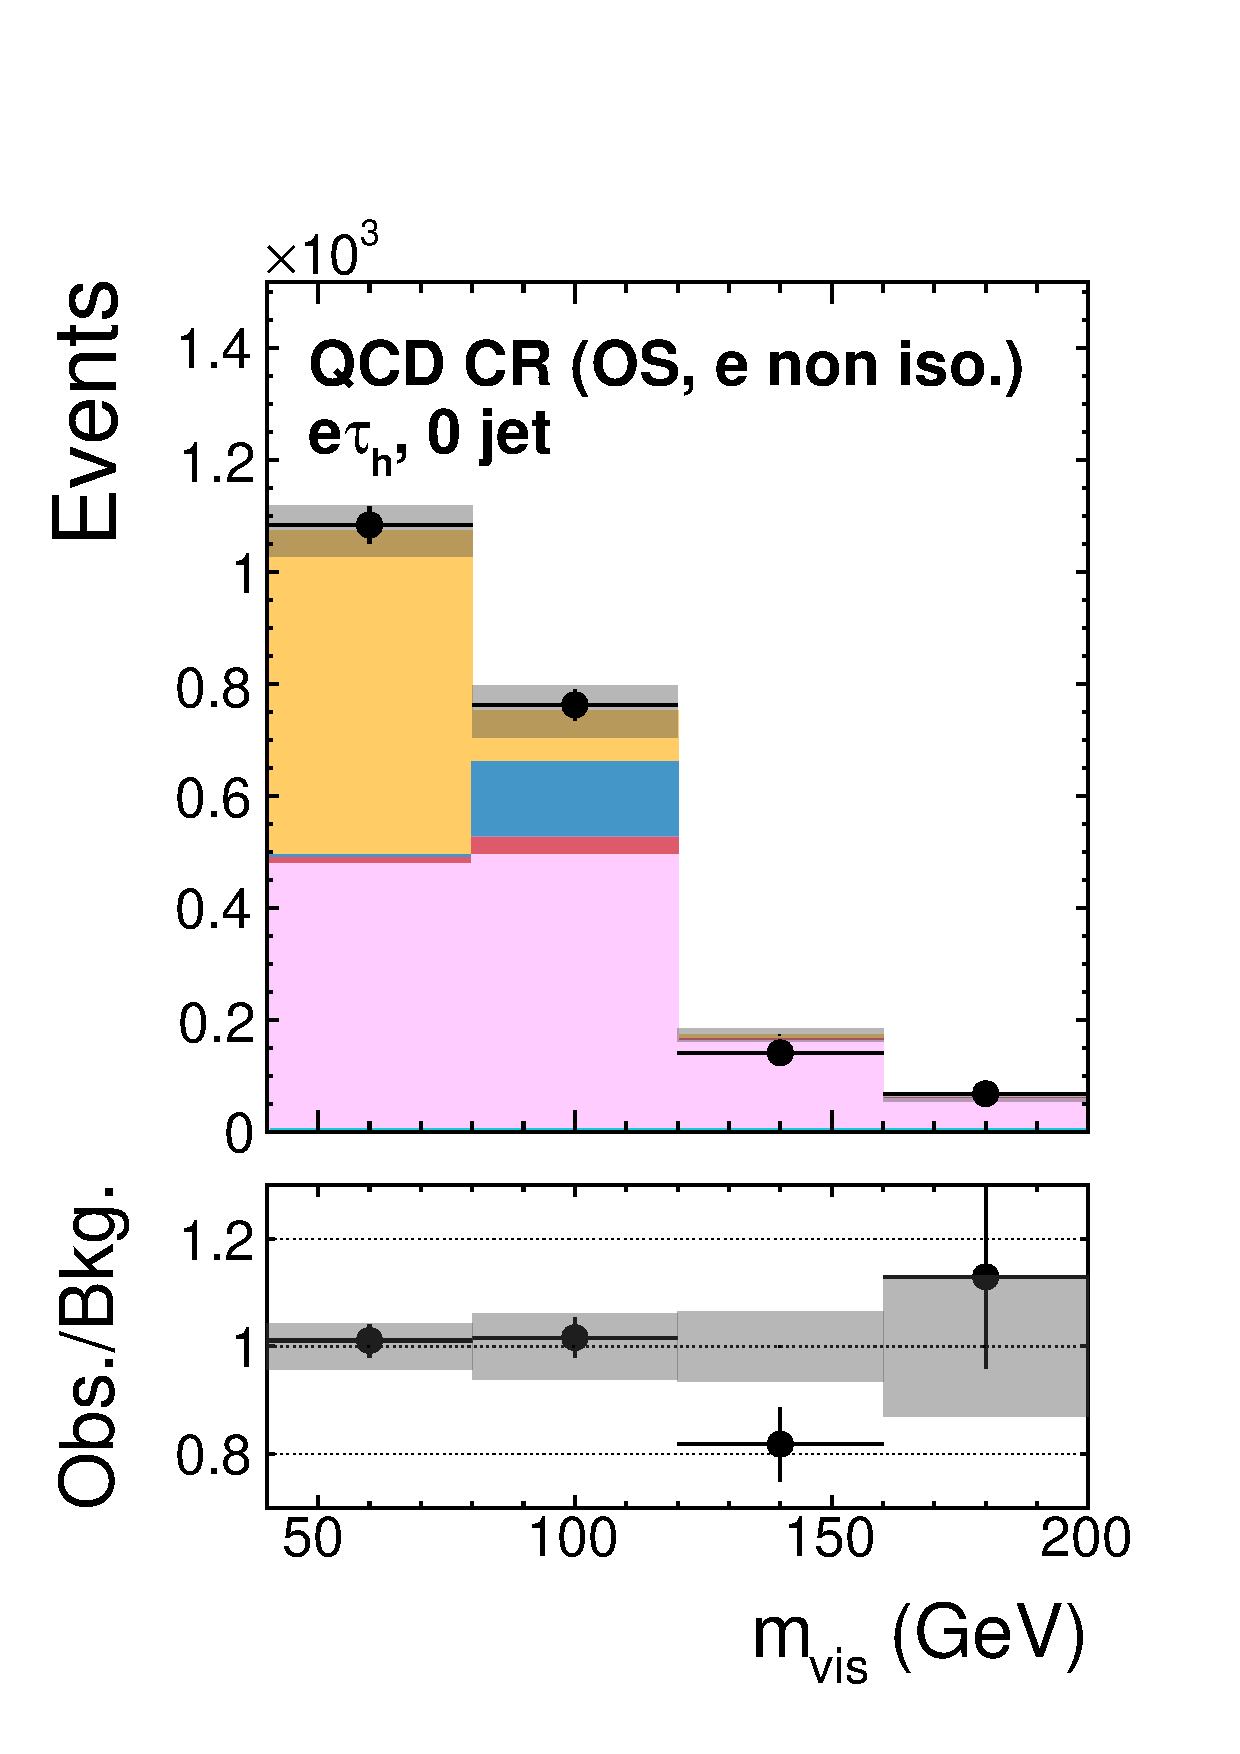
\includegraphics[width=0.3\textwidth]{higgs_to_taus/plots/Figure_003-d.pdf}
%     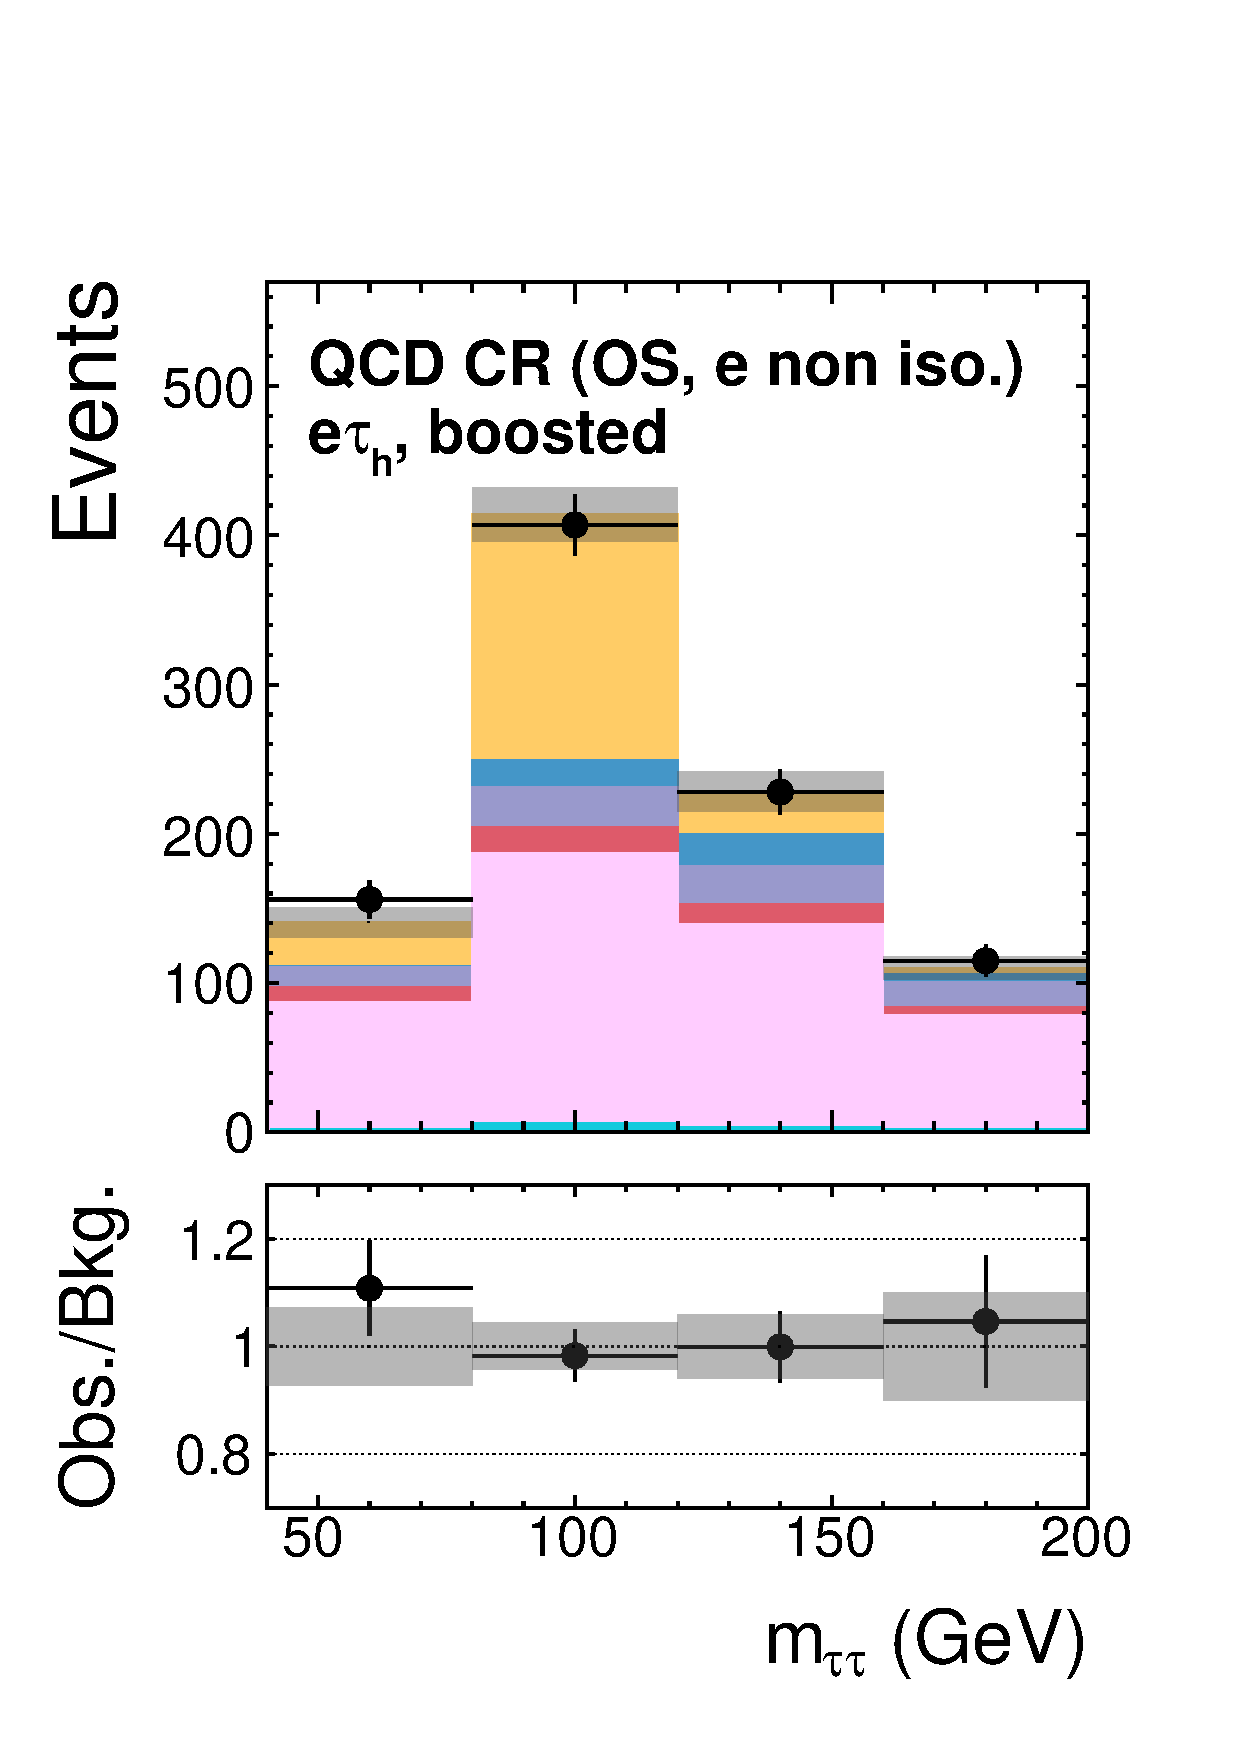
\includegraphics[width=0.3\textwidth]{higgs_to_taus/plots/Figure_003-e.pdf}
%     \caption{Control regions enriched in the QCD multijet background used in the maximum likelihood fit, together with the signal regions, to extract the results. The normalization of the predicted background distributions corresponds to the result of the global fit. These regions, defined by selecting events with opposite-sign $\ell$ and $\tauh$ candidates with $\ell$ passing inverted isolation conditions,  control the
%yields of the QCD multijet background in the $\Pgm\tauh$ and $\Pe\tauh$ channels.  The constraints obtained in the boosted categories are propagated to the VBF categories of the corresponding channels.}
%     \label{fig:htt_qcd_CR3}
%\end{figure*}

In the $\tauh\tauh$ channel, the large QCD multijet background is estimated differently than
the other channels. Comparing the QCD multijet shape templates derived using equation~\ref{eqn:qcd_eqn} 
in the same-sign region to the opposite-sign region shows inconsistencies between the expected shapes.
The Kolmogorov-Smirnov (KS) test was used to assess the level of agreement or disagreement
between the two compared QCD multijet templates. The KS test is a useful tool for comparing
the compatibility of two shape templates and is a nonparametric test of the compatibility
of continuous, one-dimensional probability distributions. Specifically, this study relied
on a two sample, binned KS test which tested the compatibility of the QCD multijet
estimated background in the same-sign region with that estimated in the opposite-sign region.
In addition, QCD multijet templates templates where tested for compatibility with both templates
defined in the same-sign region, but having differeing isolation requirement. This same check
was also done in the opposite-sign region. Table~\ref{tab:htt_qcd_ks} summarizes the results of
these KS test comparisons. It can be seen that QCD multijet shapes derived in the same-sign region
are not compatible with QCD multijet shapes derived in the opposite-sign region. And, QCD multijet
shapes derived using differing isolation requirements in the opposite-sign region show agreement
with other shapes derived in the opposite-sign region. For this reason we estimate the QCD multijet
shape template using a relaxed isolation opposite-sign side-band region.

\begin{table}[h!]
\begin{center}
{\footnotesize
\begin{tabular}{|c|c|c|}
\hline
Sign Configuration & $\tau_{h,2}$ Isolation Cuts & KS Test Value \\
\hline
%SS vs. OS & $\tau_{h,2}$!=VTight \&\& $\tau_{h,2}$==Tight & 0.033 \\
%SS vs. OS & $\tau_{h,2}$!=Tight \&\& $\tau_{h,2}$==Medium & 0.003 \\
%SS vs. OS & $\tau_{h,2}$!=Medium \&\& $\tau_{h,2}$==Loose & $<$0.001 \\
%SS vs. OS & $\tau_{h,2}$!=VTight \&\& $\tau_{h,2}$==Loose & 0.001 \\
SS vs. OS & Not VTight and Passes Tight & 0.033 \\
SS vs. OS & Not Tight and Passes Medium & 0.003 \\
SS vs. OS & Not Medium and Passes Loose & $<$0.001 \\
SS vs. OS & Not VTight and Passes Loose & 0.001 \\
\hline
\end{tabular}
\begin{tabular}{|c|c|c|c|}
\hline
Charge Config. & $\tau_{h,2}$ Iso. Cuts Shape 1 & $\tau_{h,2}$ Iso. Cuts Shape 2 & KS Test Value \\
\hline
%OS & $\tau_{h,2}$!=Tight \&\& $\tau_{h,2}$==Medium & $\tau_{h,2}$!=VTight \&\& $\tau_{h,2}$==Tight & 0.168 \\
%OS & $\tau_{h,2}$!=Medium \&\& $\tau_{h,2}$==Loose & $\tau_{h,2}$!=Tight \&\& $\tau_{h,2}$==Medium & 0.104 \\
%OS & $\tau_{h,2}$!=Medium \&\& $\tau_{h,2}$==Loose & $\tau_{h,2}$!=VTight \&\& $\tau_{h,2}$==Tight & 0.543 \\
OS & Not Tight and Passes Medium & Not VTight and Passes Tight & 0.168 \\
OS & Not Medium and Passes Loose & Not Tight and Passes Medium & 0.104 \\
OS & Not Medium and Passes Loose & Not VTight and Passes Tight & 0.543 \\
\hline
%SS & $\tau_{h,2}$!=Tight \&\& $\tau_{h,2}$==Medium & $\tau_{h,2}$!=VTight \&\& $\tau_{h,2}$==Tight & 0.587 \\
%SS & $\tau_{h,2}$!=Medium \&\& $\tau_{h,2}$==Loose & $\tau_{h,2}$!=Tight \&\& $\tau_{h,2}$==Medium & 0.036 \\
%SS & $\tau_{h,2}$!=Medium \&\& $\tau_{h,2}$==Loose & $\tau_{h,2}$!=VTight \&\& $\tau_{h,2}$==Tight & 0.029 \\
SS & Not Tight and Passes Medium & Not VTight and Passes Tight & 0.587 \\
SS & Not Medium and Passes Loose & Not Tight and Passes Medium & 0.036 \\
SS & Not Medium and Passes Loose & Not VTight and Passes Tight & 0.029 \\
\hline
\end{tabular}
}
\end{center}
\caption{
Kolmogrov-Smirnov test results comparing estimated QCD multijet shape templates to test shape compatibility
between different possible QCD multijet shape estimation regions. The $\tauh$ MVA isolation selection
for each comparison is listed where ``VTight'' means \texttt{Very Tight Tau MVA}, ``Tight'' means \texttt{Tight Tau MVA},
``Medium'' means \texttt{Medium Tau MVA}, and ``Loose'' means \texttt{Loose Tau MVA}.
In these comparisons the isolation of the highest $\pt$ $\tauh$, $\tau_{h,1}$,
is kept at \texttt{Medium Tau MVA} isolation.  
The upper table shows comparisons between same-sign (SS) and opposite-sign (OS) selections for the same
exact isolation selection. The lower table shows KS test results for comparisons
within the same charge configuration across different isolation requirements.
}
\label{tab:htt_qcd_ks}
\end{table} 

The selection for estimating the QCD multijet background shape template and raw yeild requires 
that at least one of the $\tauh$
must fail the \texttt{Tight Tau MVA} requirement which is the isolation selection used to 
define the signal region. This selection
ensures that the side-band sample is disjoin from the signal region.
In this region, the QCD multijet background shape and raw yield are obtained
by subtracting the contribution of the Drell--Yan, \ttbar, and $\PW+\text{jets}$ processes, 
estimated from simulation as explained above, from the data as in eqn~\ref{eqn:qcd_eqn}.

A scaling factor is required to adjust the raw yield estimated above to the expected
QCD multijet yield in the signal extraction region. This extrapolation factor
is estimated in the same-sign charge region. Two same-sign QCD multijet samples are constructed
using 1) the exact same isolation requirements as the signal region; all selections are identical
here except for the $\tauh$ charge configuration. And, 2) a second region with the exact 
same relaxed isolation requirements as the region used to estimate the opposite-sign
QCD multijet shape template and raw yield. From these two samples a ``Relaxed-Region-to-Signal-Region''
scaling factor is calculated as,
\[ \text{Relaxed-Region-to-Signal-Region SF} = \frac{\text{Signal Region Yield}}{\text{Relaxed Region Yield}} \]
Multiplying the raw yield estimated above by this scaling factor results in the estimated
QCD multijet contribution in the signal region. The ``Relaxed-Region-to-Signal-Region'' scale factors
for the three $\tauh\tauh$ categories are listed in table~\ref{tab:htt_qcd_sf}. The uncertainties associated
with these scale factors are propagated through the QCD multijet estimation process and combined
with results from closure tests to estimate a final category dependant systematic and statistic uncertainty
for the QCD multijet estimation process.

\begin{table*}[htbp]
\centering
\begin{tabular}{|l|c|}
\hline
Category   &   ``Relaxed-Region-to-Signal-Region''   \\
           &   Scale Factor   \\
\hline
0-jet      &    0.25 $\pm$ 1.0\%  \\
VBF        &    0.18 $\pm$ 10\%  \\
Boosted    &    0.23 $\pm$ 1.4\%  \\  
\hline
\end{tabular}
\label{tab:htt_qcd_sf}
\caption{
The category dependant scale factors used to adjust the QCD multijet yield to correspond 
to the expected yield in the signal region. The large uncertainty on the VBF scale factor show the
limited amount of QCD multijet events in the VBF same-sign region. 
}
\end{table*}

The events selected with opposite-sign $\tauh$ candidates passing relaxed isolation requirements 
form control regions, shown in Fig.~\ref{fig:htt_qcd_CR4}, and are used in the global fit to extract the results.

\begin{figure*}[!htbp]
\centering
     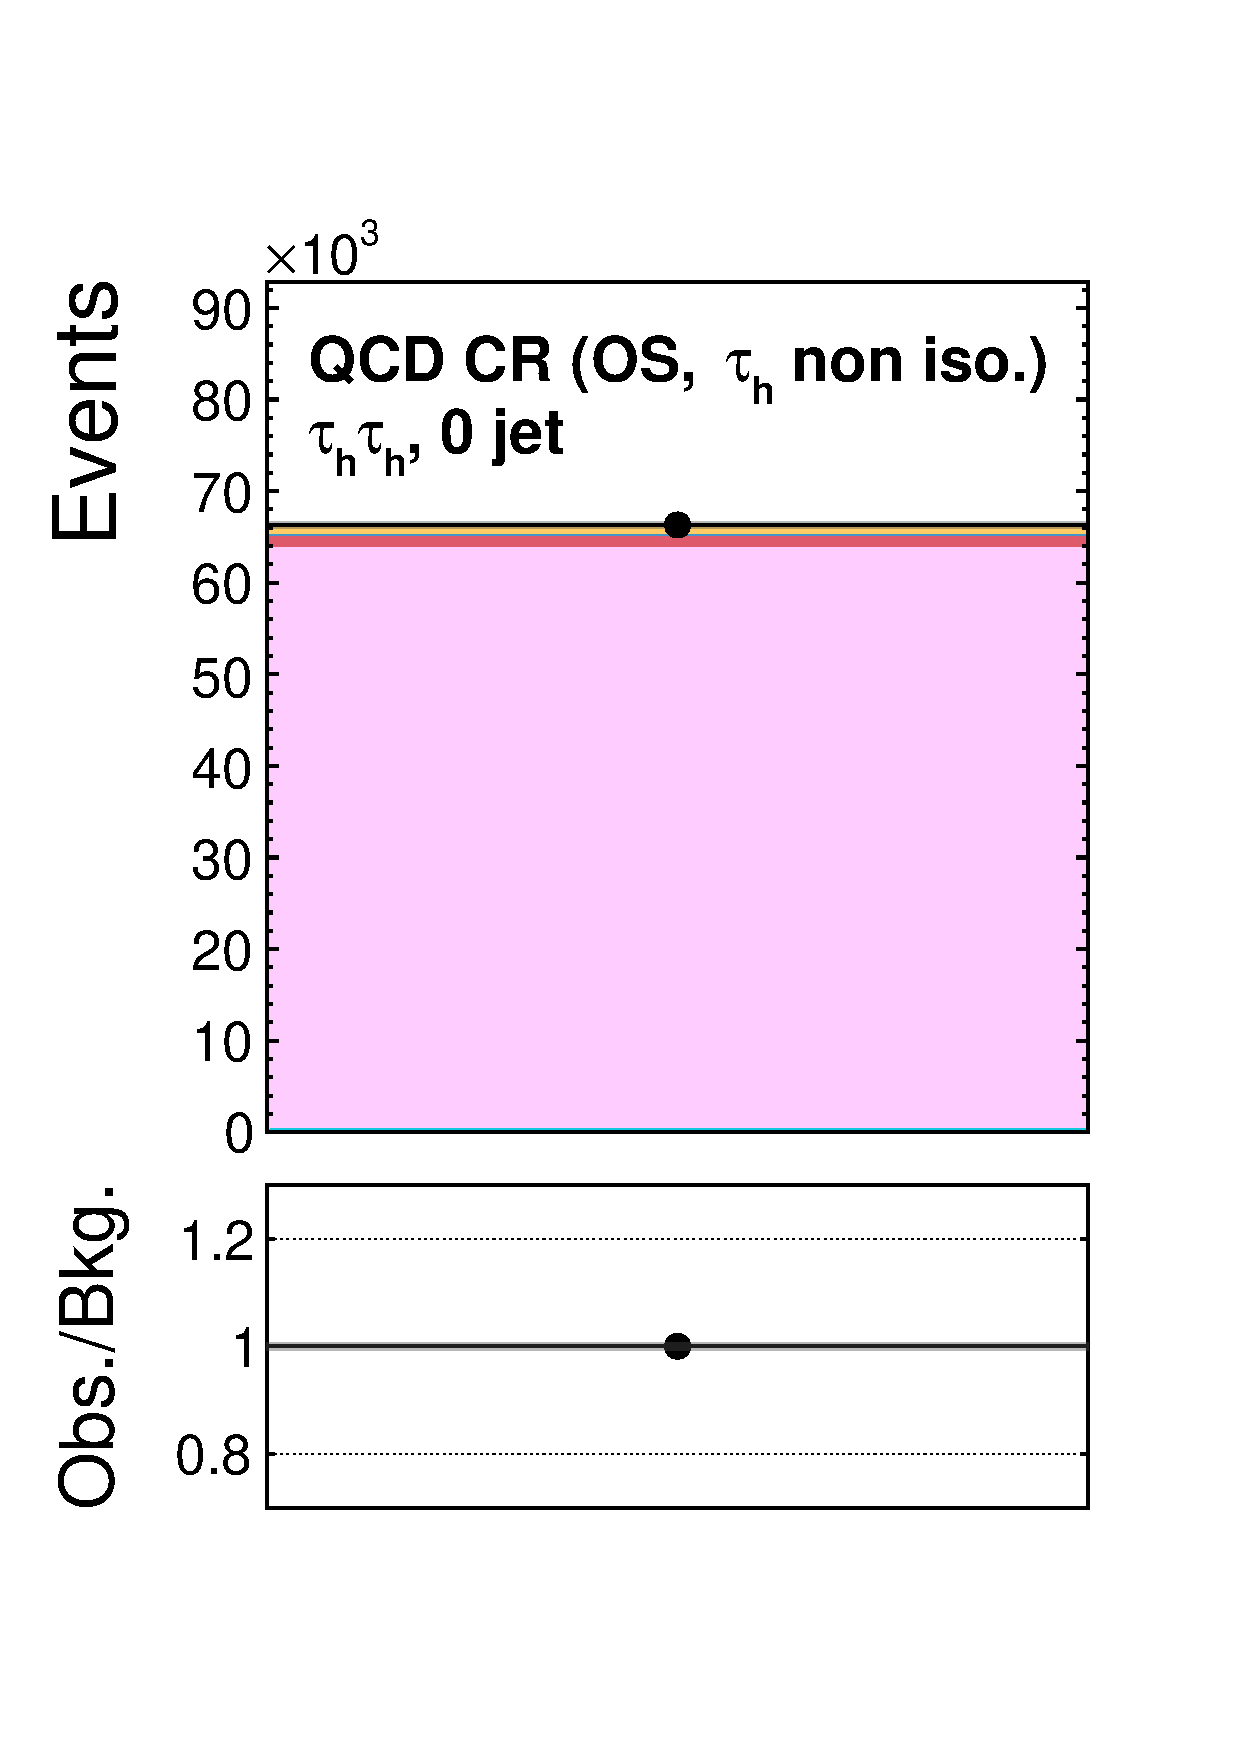
\includegraphics[width=0.24\textwidth]{higgs_to_taus/plots/Figure_004-a.pdf}
     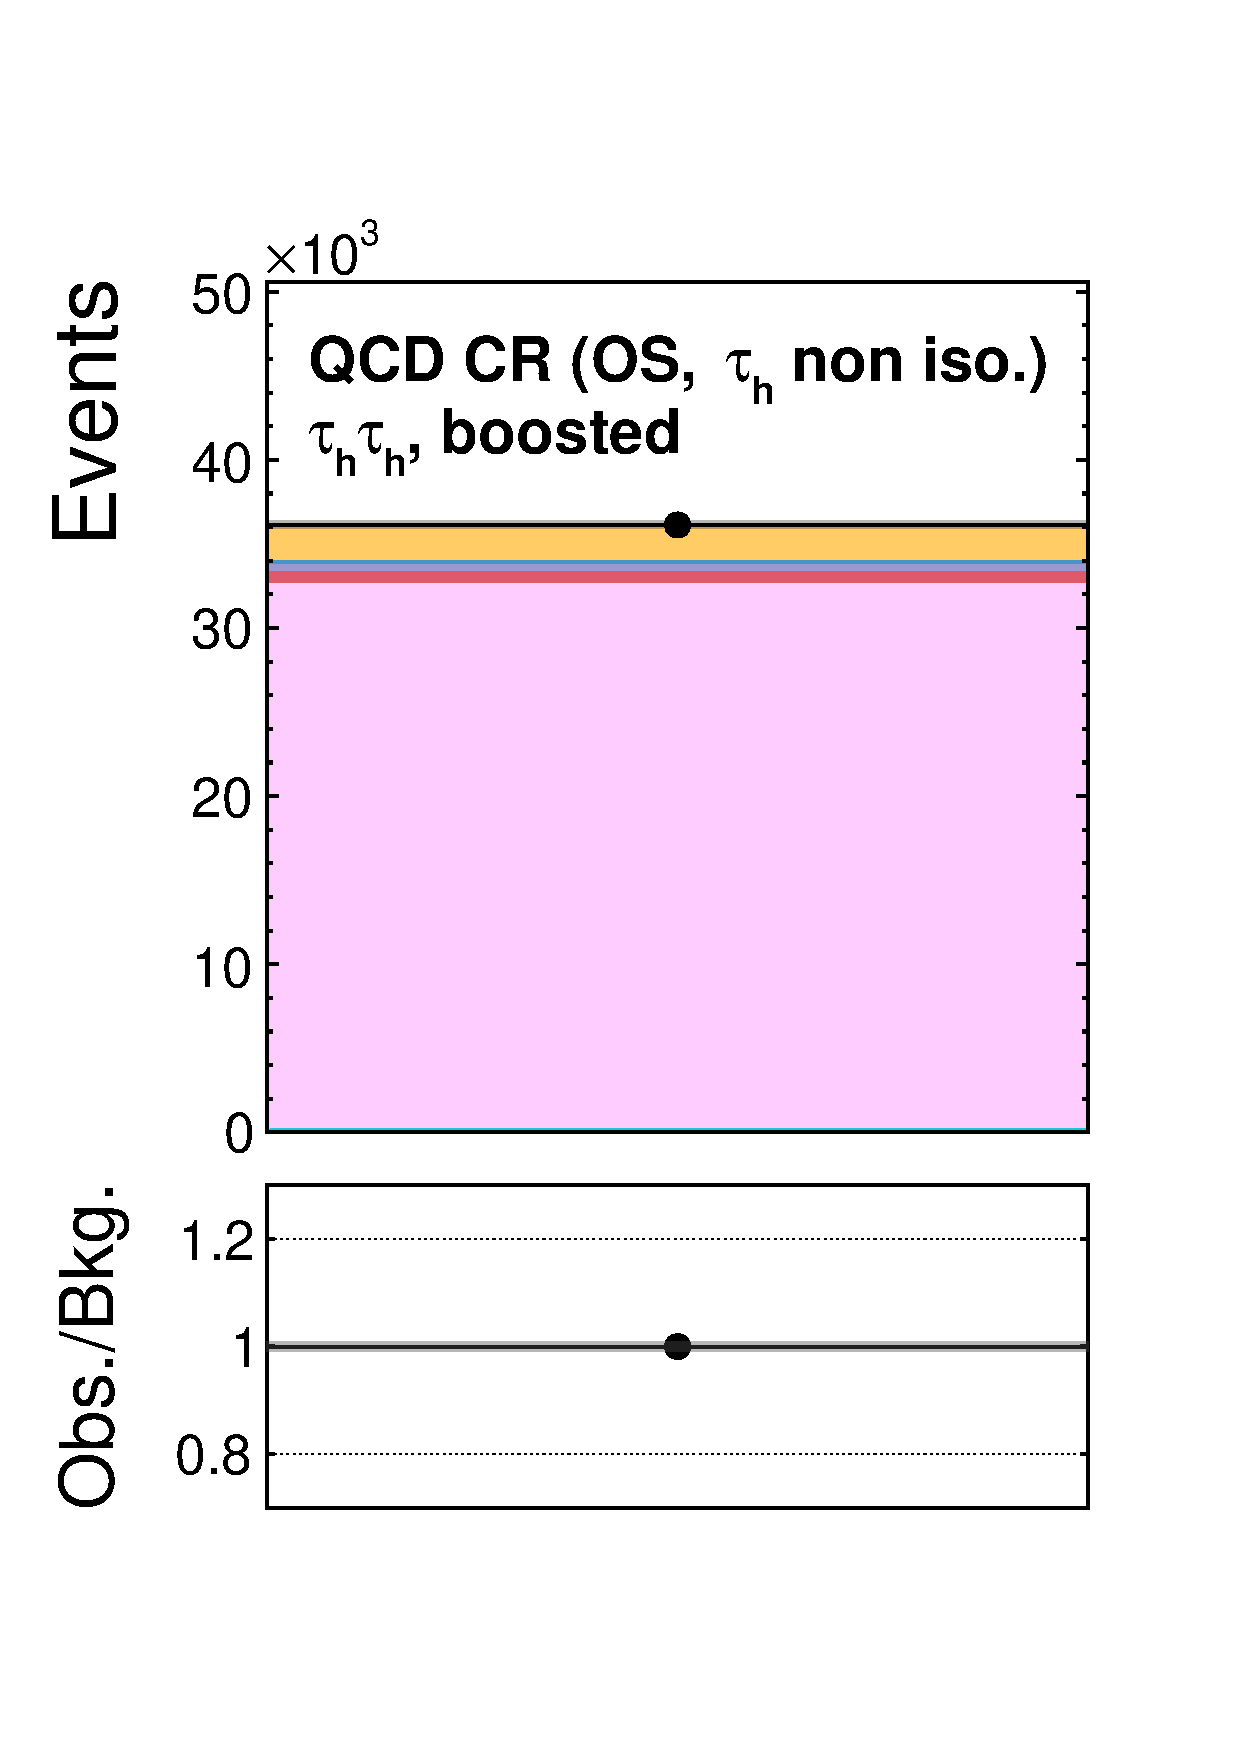
\includegraphics[width=0.24\textwidth]{higgs_to_taus/plots/Figure_004-b.pdf}
     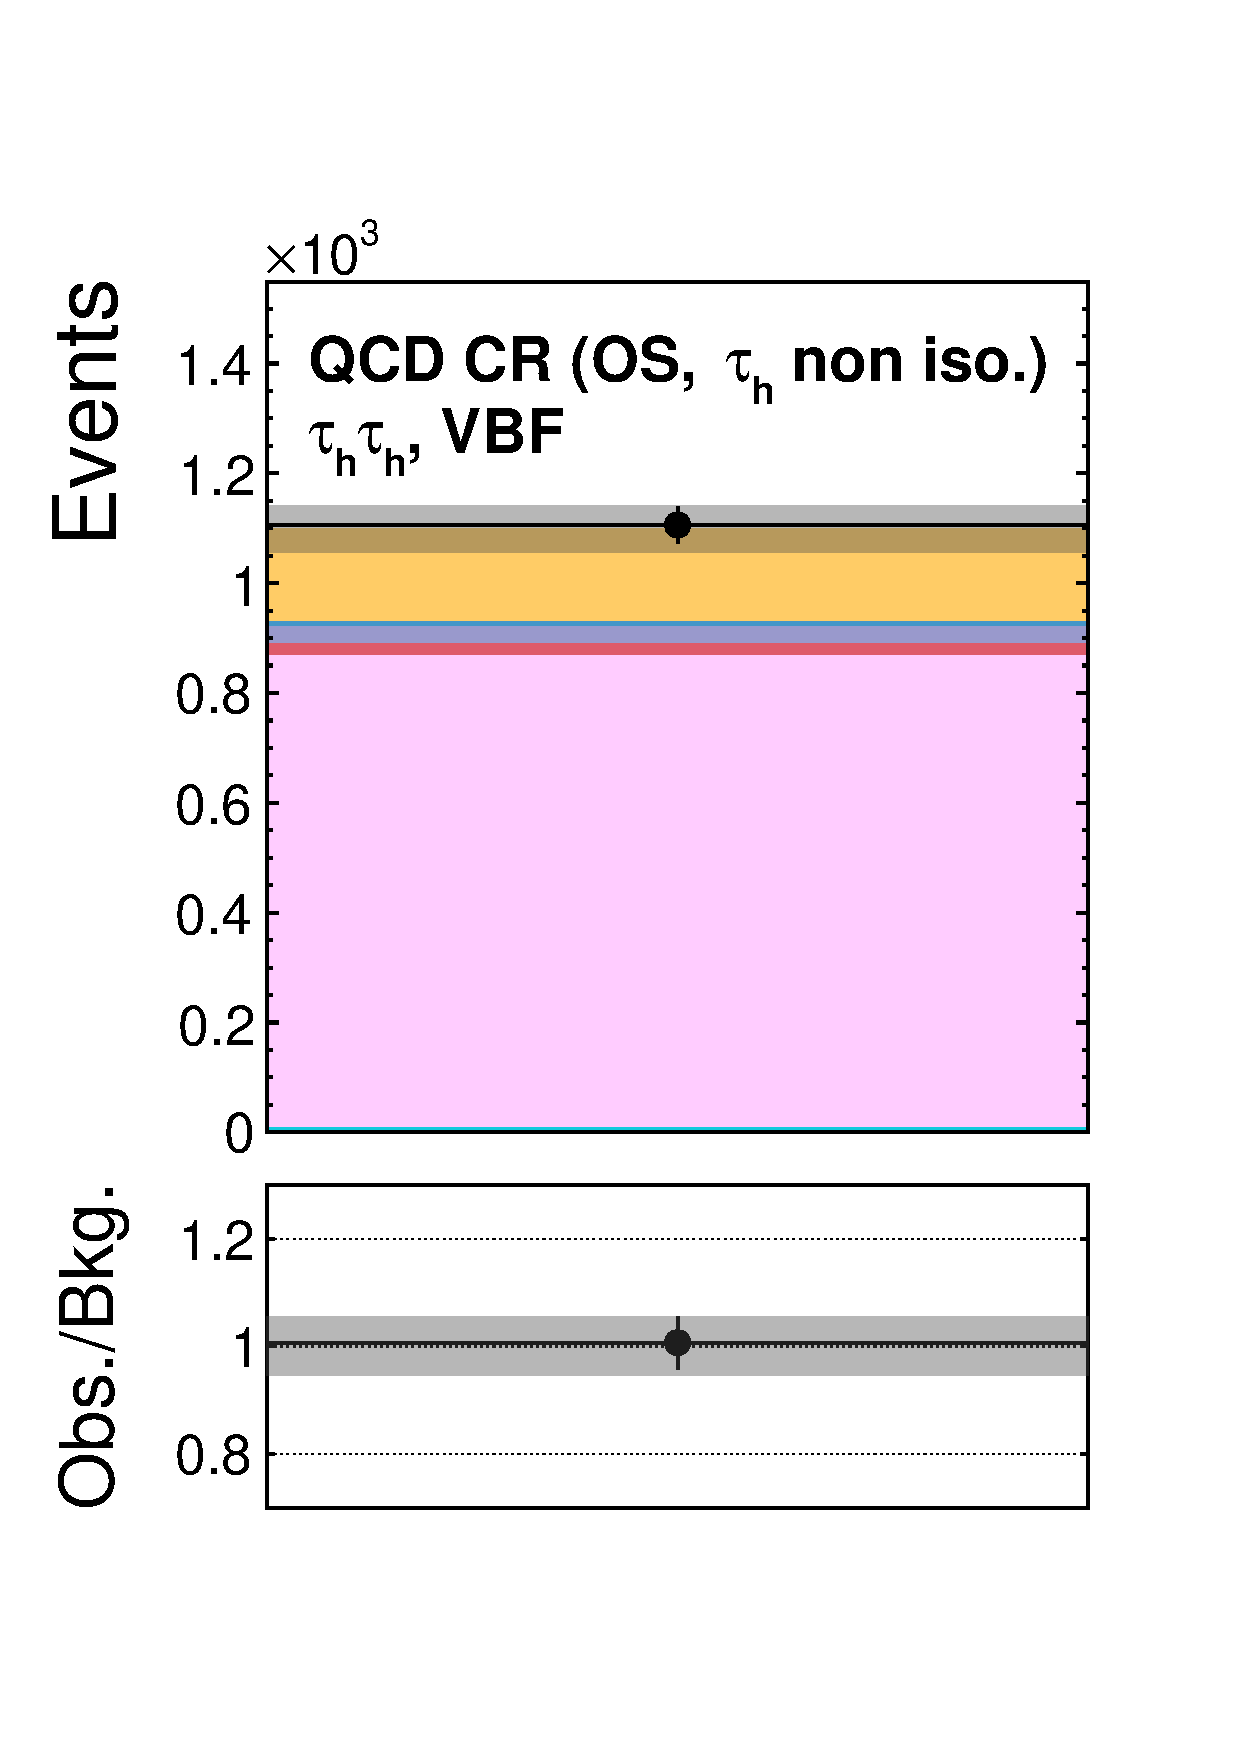
\includegraphics[width=0.24\textwidth]{higgs_to_taus/plots/Figure_004-c.pdf}
     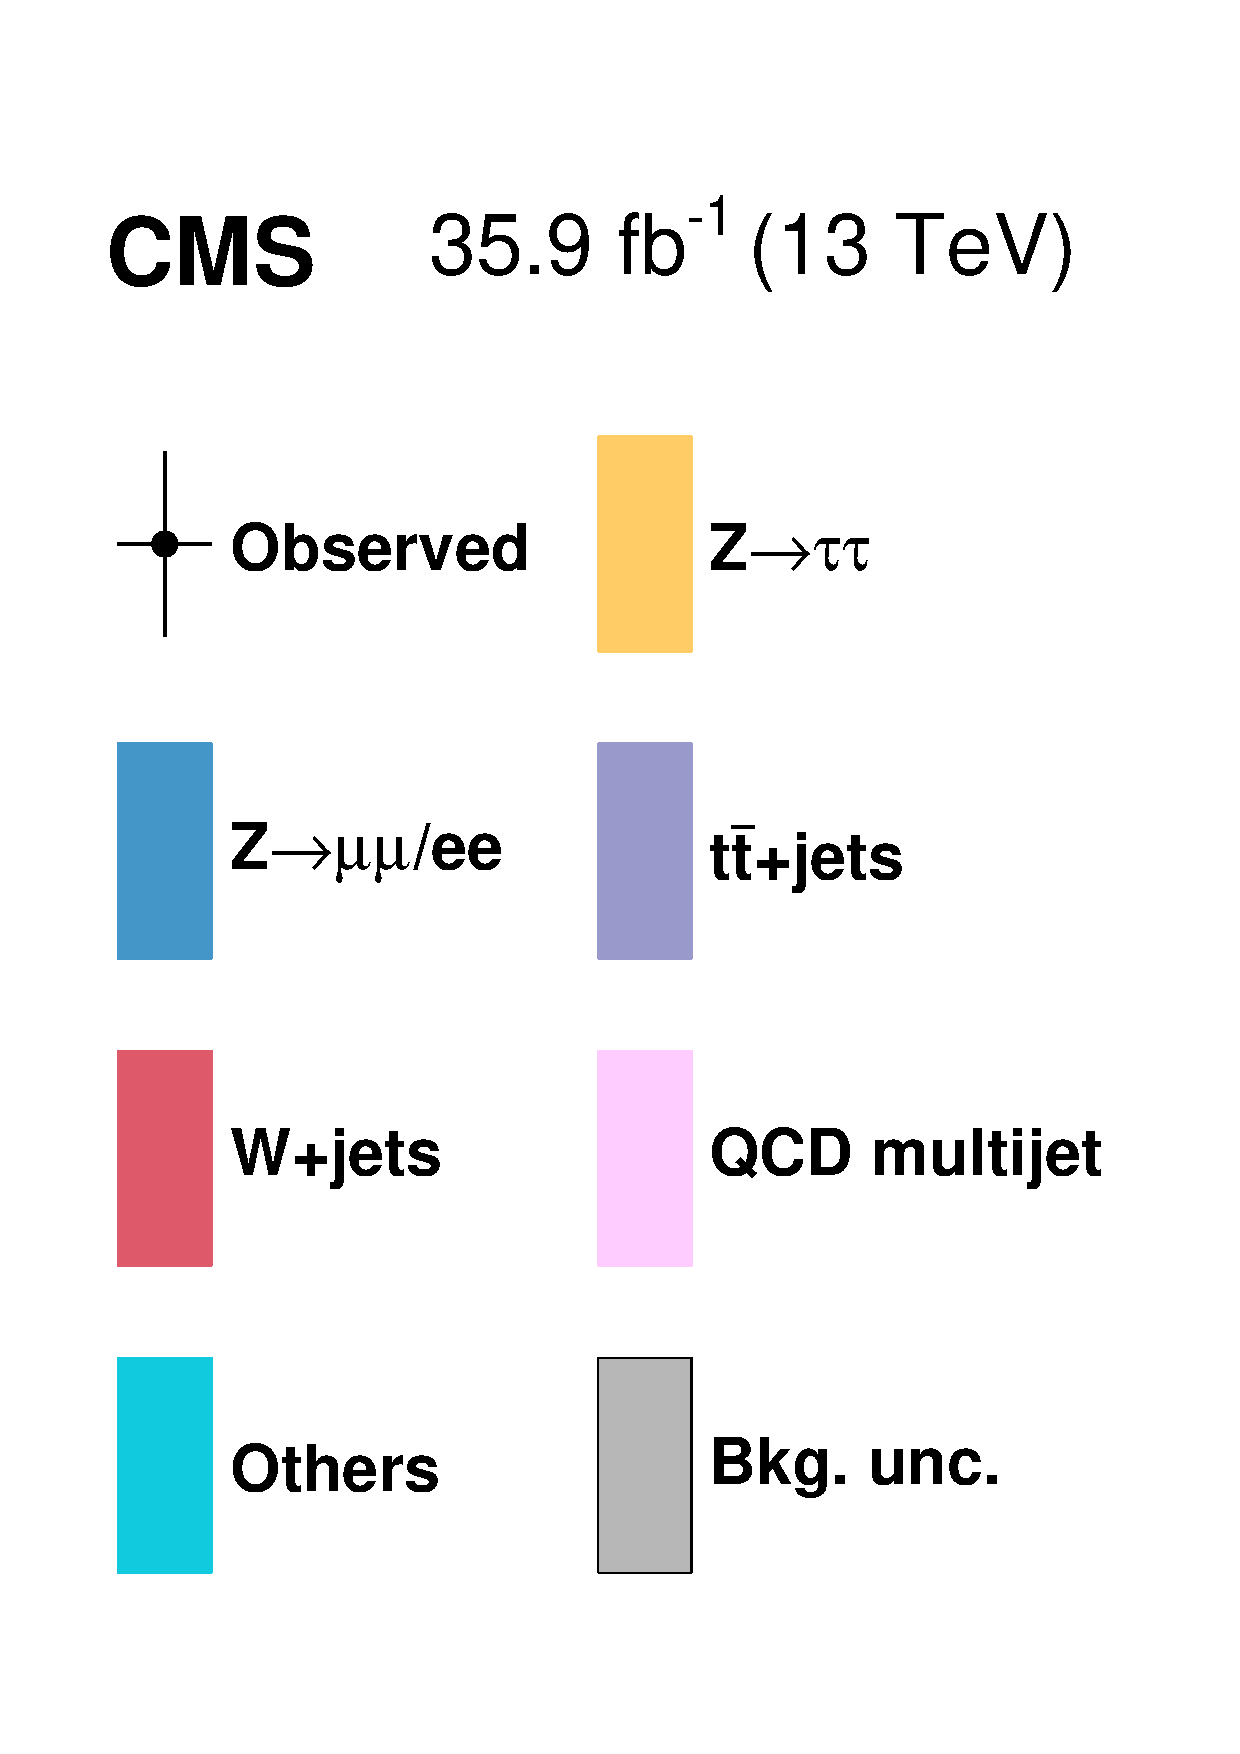
\includegraphics[width=0.24\textwidth]{higgs_to_taus/plots/Figure_004-d.pdf}
     \caption{Control regions enriched in the QCD multijet background used in the maximum likelihood fit, 
together with the signal regions, to extract the results. The normalization of the predicted background 
distributions corresponds to the result of the global fit. These regions, a formed by selecting events with 
opposite-sign $\tauh$ candidates passing relaxed isolation requirements with at least one of them
failing \texttt{Tight Tau MVA} isolation. These regions control the yields of the QCD multijet background 
in the $\tauh\tauh$ channel.}
     \label{fig:htt_qcd_CR4}
\end{figure*}



The \ttbar production process is one of the main backgrounds in the $\Pe\Pgm$ channel.
In all channels \ttbar is predicted from simulation. The normalization is adjusted in
A \ttbar-enriched sample orthogonal to the signal region provides a control region which is included
in the global fit. The \ttbar control region is defined from the $\Pe\Pgm$ channel. The yield
of \ttbar in all channels and categories is adjusted by the \ttbar control region.
This control region, shown in Fig.~\ref{fig:htt_ttbar_CR2},
The selection enforming orthagonality from the $\Pe\Pgm$ signal region is inverting the $p_\zeta$ requirement
and the events should contain at least one jet.

\begin{figure}[htb]
\centering
     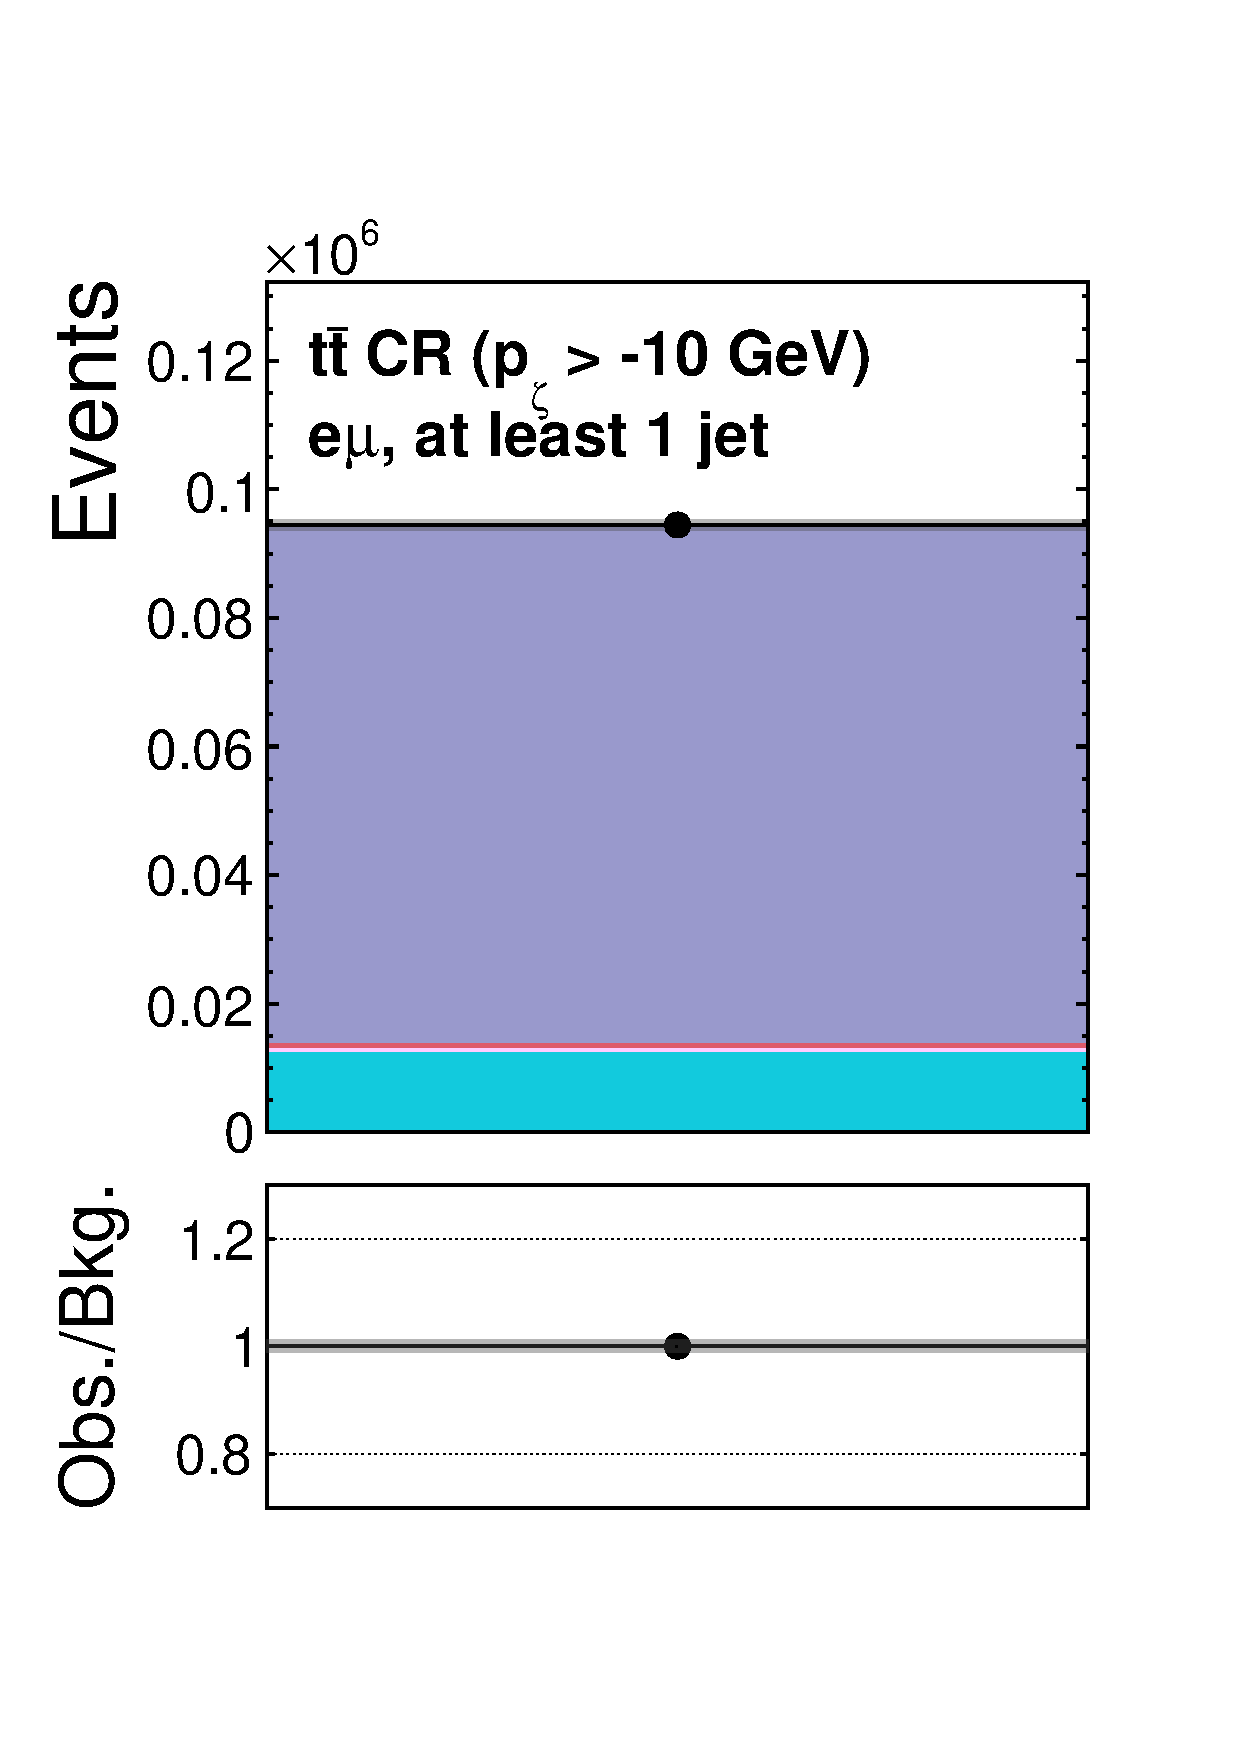
\includegraphics[width=0.23\textwidth]{higgs_to_taus/plots/Figure_005-a.pdf}
     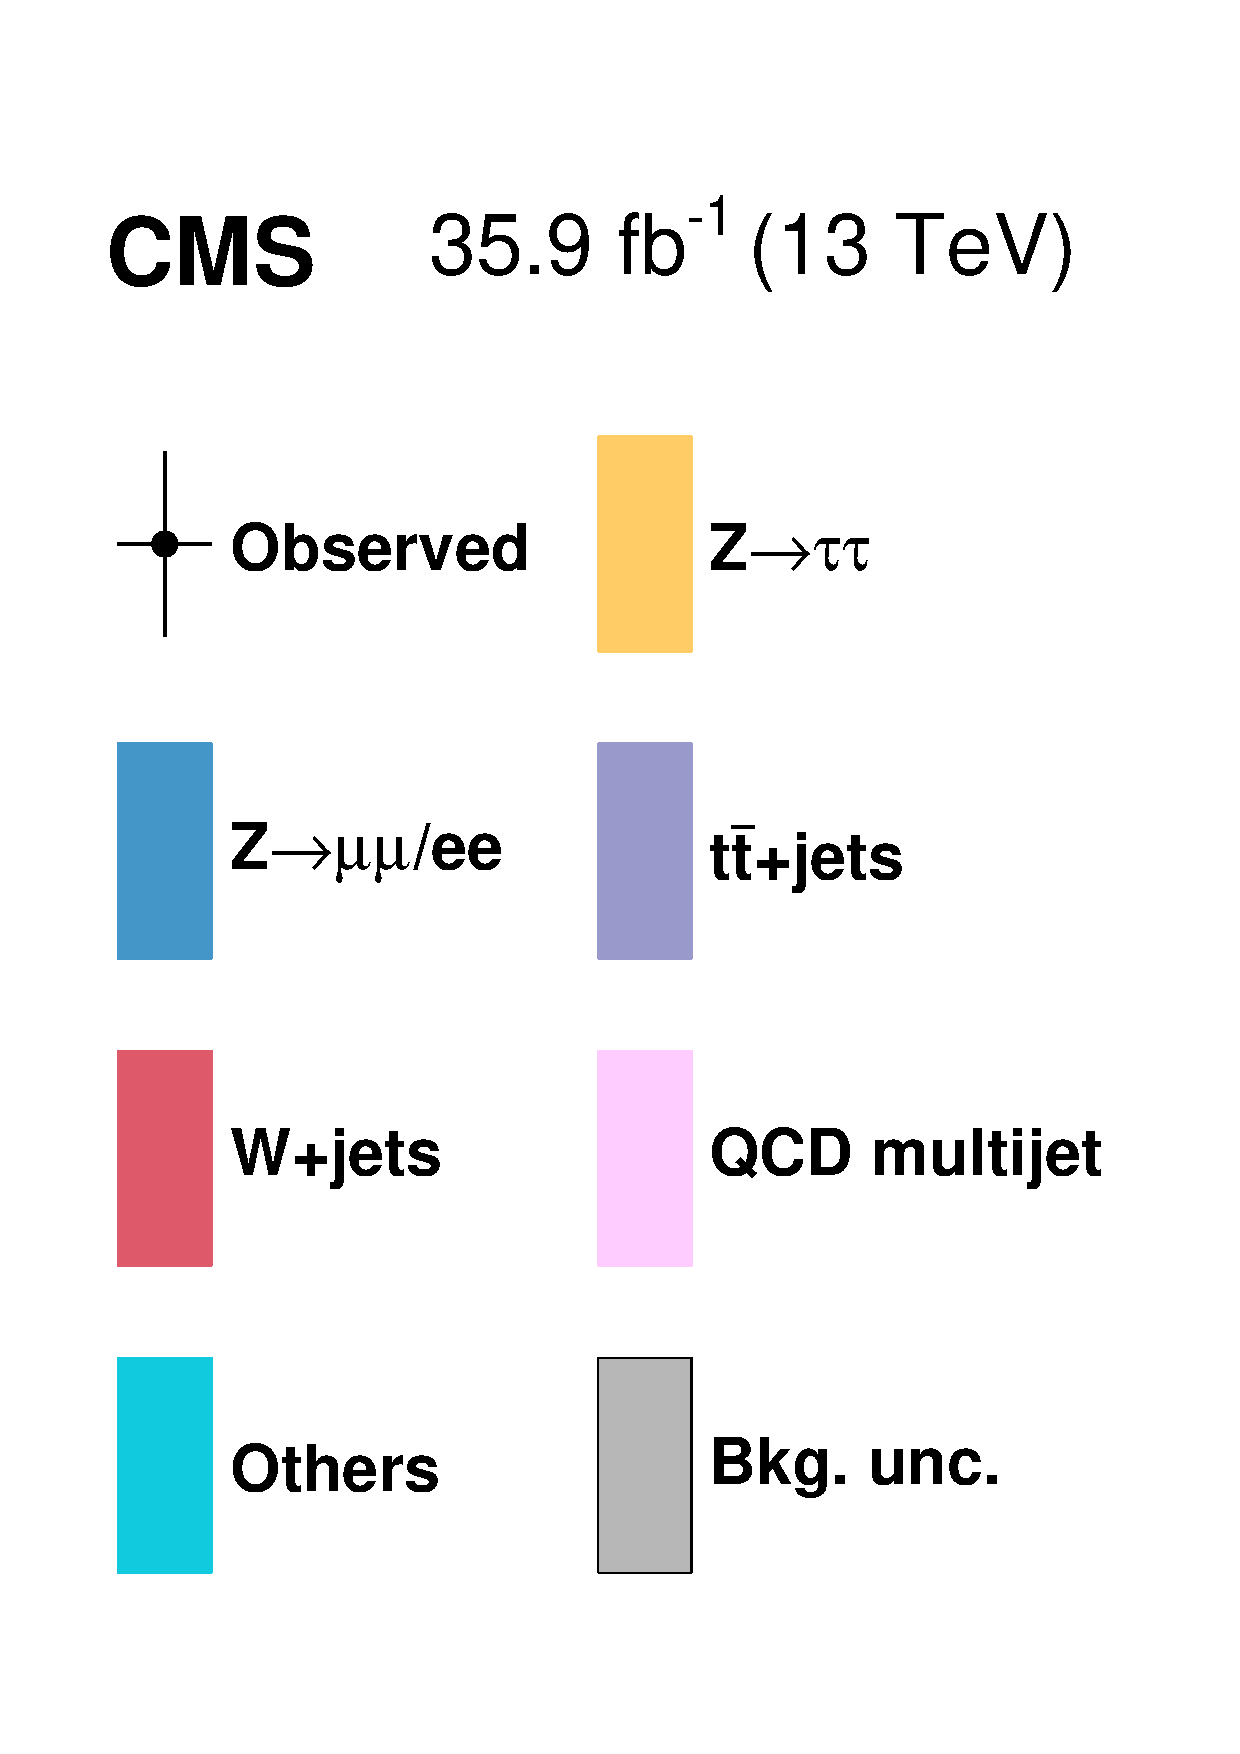
\includegraphics[width=0.23\textwidth]{higgs_to_taus/plots/Figure_005-b.pdf}
     \caption{Control region enriched in \ttbar background, used in the maximum likelihood fit, 
together with the signal regions, to extract the results. The normalization of the predicted background 
distributions corresponds to the result of the global fit. This region, defined by inverting the 
$p_\zeta$ requirement and rejecting events with no jet in the $\Pe\Pgm$ final state, is used to estimate the
yields of the \ttbar background in all channels.}
     \label{fig:htt_ttbar_CR2}
\end{figure}

Other background processes, such as, contributions from diboson and single top quark production, are estimated 
from simulation.

\pagebreak

\section{Monte Carlo Corrections}
\label{sec:mc_corrections}

Corrections are applied to the simulated Monte Carlo samples to help correct for measured differences
between observed data and expectations based on simulation. Many of these corrections are designed
to correct differences in reconstruction and identification efficiencies for objects between data
and simulation. These corrections are derived in
fully orthogonal regions from the analysis signal regions when ever possible. There are however many
instances where the $\Pgm\tauh$ channel is used to derive corrections. In these cases the measurement
region used to derive corrections will overlap with a subset of the analysis signal regions. This
overlap is discussed in the Systematic Uncertainties section~\ref{sec:htt_systematics}.


\subsection{Pileup Reweighting}
During 2016 data taking, the LHC delivered \pp collisions to CMS with an average of approximately 27
interactions per bunch crossing. Monte Carlo samples are generated with additional pileup interactions
added to the hard-scattering process for each event. A reweighting technique is used which improves
the aligment between the pileup interactions in data and those in Monte Carlo. This is critical because
there are some reconstructed event characteristics such as \etvecmiss which can be influenced by the
number of pileup interactions per event.


\subsection{Tau Identification Efficiency}
The reconstruction efficiency for hadronically decaying taus is observed to be different in data and in simulated samples.
Correction factors are derived by the Tau POG using the $\Pgm\tauh$ channel using a tag-and-probe method. Essentially,
the Tau ID Efficiency measurement selects $\PZ/\Pgg^*\to\Pgt\Pgt\to\Pgm\tauh$ events on the $\PZ$
mass peak and performs a fit with the $\PZ\to\Pgm\tauh$ process treated as a signal. The degree
to which the $\PZ\to\Pgm\tauh$ process is scaled up to down is the resulting Tau ID Efficiency
scale factor. The measured scale factor is 0.95 $\pm$ 0.05 for all $\tauh$ passing \texttt{Tight Tau MVA}.
This correction factor is applied to all simulated $\tauh$ which are matched at the generator
level to $\tau$ leptons.


\subsection{Tau Energy Correction}




\subsection{Lepton Identification and Isolation Efficiencies}
Similar to the Tau ID Efficiency measured above, the electron and muon reconstruction, identification,
and isolation efficiencies are measured in both data and simulation. Correction factors equal to
$\epsilon_{data}/\epsilon_{MC}$ are derived as a function of both lepton $\pt$ and lepton $\eta$.
The electron (muon) efficiencies are measured in $\PZ\to\Pe\Pe$ ($\PZ\to\Pgm\Pgm$) events using a tag-and-probe
method.


\subsection{Trigger Efficiencies}
Trigger efficiencies are measured in data and in simulation for all of the channels. For the channels
which trigger on $\tauh$, the $\Pgm\tauh$ and $\tauh\tauh$ channels, the $\tauh$ efficiency is measured
using tag-and-probe in the $\Pgm\tauh$ final state. The efficiencies for the $\tauh\tauh$ channel
are measured with dedicated muon+$\tauh$ monitoring triggers. The $\tauh$ trigger requirements
are identical between the monitoring trigger and the $\tauh\tauh$ trigger paths. The tag-and-probe
is conducted using the Single Muon PD. The selection for the $\tauh$ trigger efficiency measurements 
requires one well identified and isolated muon per event. The muon is required to fire a single muon trigger.
Events with at least one $\tauh$ which passes \texttt{decay mode finding} and \texttt{Tight Tau MVA} isolation
constitute the denominator selection for the efficiency measurement. Events where the $\tauh$
fires the trigger under study are recorded as passing events. The ratio of passing events to
denominator events defines the trigger efficiency. Trigger efficiencies for are measured and applied as 
a function of $\tauh$: $\pt$, decay mode, and generator matching status. Figure~\ref{fig:htt_tt_trig}
shows the trigger efficiency versus $\pt$ for the double-$\tauh$ trigger.

\begin{figure*}[!htbp]
\centering
     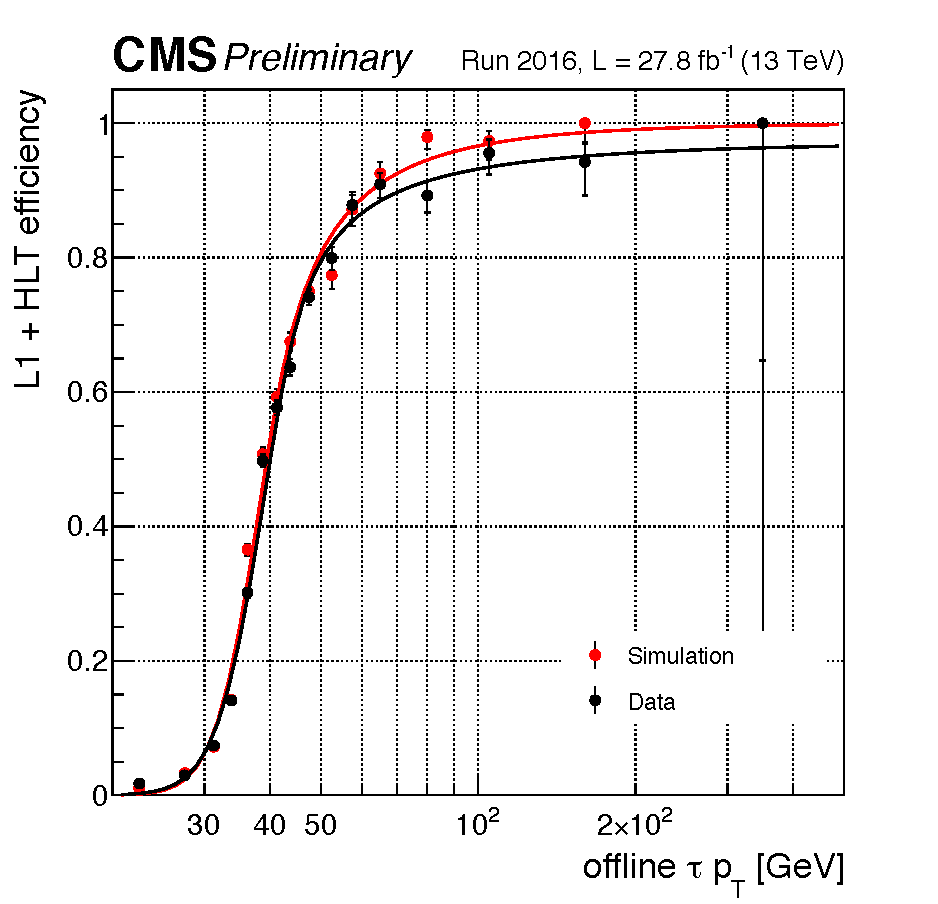
\includegraphics[width=0.65\textwidth]{higgs_to_taus/plots/htt_tautau_trigger_efficiency.pdf}
     \caption{
Comparison of the trigger efficiencies for the \texttt{HLT\_DoubleMediumIsoPFTau35\_Trk1\_eta2p1\_Reg}
which was active in data during eras B-G. The efficiency was measured using tag-and-probe in the
$\Pgm\tauh$ final state. The efficiency is measured for a single leg of the double-$\tauh$ at a time
with a muon+$\tauh$ monitoring trigger. The efficiencies shown here are used in the $\tauh\tauh$ channel.
The specific distribution shown is for real $\tau$ leptons and includes all used decay modes.
}
     \label{fig:htt_tt_trig}
\end{figure*}

The trigger efficiencies for electrons and muons are also measured with a tag-and-probe method.
Similar to the electron and muon identification and isolation efficiencies, the 
electron (muon) efficiencies trigger are measured in $\PZ\to\Pe\Pe$ ($\PZ\to\Pgm\Pgm$) events.
The denominator selection for the probe lepton requires that the same identification and
isolation criteria used in the analysis be met. The efficiencies are measured as a function of
lepton $\pt$ and $\eta$.



\subsection{Drell--Yan Reweighting}

The simulated Monte Carlo Drell--Yan sample used in the analysis is simulated at leading order (LO)
using the \aMCATNLO generator discussed in section~\ref{sec:simulation}. To assess Monte Carlo to
data agreement we use a dedicated $\PZ/\Pgg^*\to\Pgm\Pgm$ control region with high Drell--Yan purity.
The $\PZ/\Pgg^*\to\Pgm\Pgm$ control region uses events from the Single Muon PD and requires the 
presence of two well-identified muons with $\pt > 25 \GeV$ and an invariant mass between 70 and 110\GeV.
With this selection criteria over 99\% of the events are attributed to $\PZ/\Pgg^*\to\Pgm\Pgm$ decays.

Differences in the distributions of $m_{\ell\ell/\Pgt\Pgt}$ and $\pt(\ell\ell/\Pgt\Pgt)$ between data and 
in simulations are observed in this control region. To correct for this, 2D weights based on these variables 
are derived and applied to simulated $\PZ/\Pgg^*\to\Pgt\Pgt, \ell\ell$ events in the signal region of the analysis. 
In addition, corrections depending on $\mjj$ are derived from the $\PZ/\Pgg^*\to\Pgm\Pgm$ region and 
applied to the $\PZ/\Pgg^*\to\Pgt\Pgt, \ell\ell$ simulation for events with at least two jets passing the 
VBF category selection criteria. After this reweighting, good agreement between data in the 
$\PZ/\Pgg^*\to\Pgm\Pgm$ region and simulation is found for all other variables used in the analysis.
These derived corrections are also applied to the simulated samples of electroweak production of $\PZ$ 
bosons. Electroweak produced $\PZ$ contributes up to 8\% of the $\PZ$ boson production in the VBF category.



\subsection{Recoil Corrections}



\subsection{Generator Event Weights}
\subsection{Luminosity}

\pagebreak

\section{Systematic Uncertainties}
\label{sec:htt_systematics}

\subsection{Uncertainties related to object reconstruction and identification}

The overall uncertainty in the $\tauh$ identification efficiency for genuine $\tauh$ leptons is 5\%, 
which has been measured with a tag-and-probe method in $\PZ\to\Pgt\Pgt$ events.
This number is not fully correlated among the di-$\Pgt$ channels because the $\tauh$ candidates are required to pass
different working points of the discriminators that reduce the misidentification rate of electrons and muons as $\tauh$ candidates.
The trigger efficiency uncertainty per $\tauh$ candidate amounts to an additional 5\%, which leads to a total 
trigger uncertainty of 10\% for processes estimated from simulation in the $\tauh\tauh$ decay channel. This 
uncertainty has also been measured with a tag-and-probe method in $\PZ\to\Pgt\Pgt$ events.

An uncertainty of 1.2\% in the visible energy scale of genuine $\tauh$ leptons affects both the distributions and the
signal and background yields. It is uncorrelated among the 1-prong, 1-prong + $\PGpz$, and
3-prong decay modes.
The magnitude of the uncertainty was determined in $\PZ\to\Pgt\Pgt$ events with one $\Pgt$ lepton decaying hadronically 
and the other one to a muon, by performing maximum likelihood fits for different values of the visible energy scale of 
genuine $\tauh$ leptons. Among these events, less than half overlap with the events selected in the $\Pgm\tauh$ 
channel of this analysis. The fit constrains the visible $\tauh$ energy scale uncertainty to about
0.3\% for all decay modes. The constraint mostly comes from highly populated regions with a high $\tauh$ purity, namely 
the 0-jet and boosted categories of the $\Pgm\tauh$ and $\tauh\tauh$ channels. The decrease in the size of the 
uncertainty is explained by the addition of two other decay channels
with $\tauh$ candidates ($\tauh\tauh$ and $\Pe\tauh$), by the higher number of events in the MC simulations, and by the 
finer categorization that leads to regions with a high $\PZ\to\Pgt\Pgt$ event purity.
Even in the most boosted categories, reconstructed $\tauh$ candidates typically have moderate $\pt$ ($\pt$ less than 100\GeV) and are
found in the barrel region of the detector. As tracks are well measured in the CMS detector for this range of $\pt$,
the visible energy scale of genuine $\tauh$ leptons is fully correlated for all $\tauh$ leptons reconstructed in the 
same decay mode, irrespective of their $\pt$ and $\eta$. The uncertainties in the visible energy scale for genuine 
$\tauh$ leptons together contribute an uncertainty of 5\% to the measurement of the signal strength.

In the 0-jet category of the $\Pgm\tauh$ and $\Pe\tauh$ channels, the relative contribution of $\tauh$ in a given
reconstructed decay mode is allowed to fluctuate by 3\% to account for the possibility that the reconstruction and
identification efficiencies are different for each decay mode. This uncertainty has been measured in a region enriched 
in $\PZ\to\Pgt\Pgt$ events with one $\Pgt$ lepton decaying hadronically and the other one decaying to a muon, by 
comparing the level of agreement in exclusive bins of the reconstructed $\tauh$ decay mode, after adjusting the inclusive 
normalization of the $\PZ\to\Pgt\Pgt$ simulation to its best-fit value. The effect of migration between the reconstructed 
$\tauh$ decay modes is negligible in other categories, where
all decay modes are treated together.

For events where muons or electrons are misidentified as $\tauh$ candidates, essentially $\PZ\to \Pgm\Pgm$ events in 
the $\Pgm\tauh$ decay channel and $Z\to \Pe\Pe$ events in the $\Pe\tauh$ decay channel, the $\tauh$ identification leads 
to rate uncertainties of 25 and 12\%, respectively, per reconstructed $\tauh$ decay mode. Using $\mvis$ and the reconstructed 
$\tauh$ decay mode as the observables in the 0-jet category of the $\Pgm\tauh$ and $\Pe\tauh$ channels helps reduce the 
uncertainty after the signal extraction fit: the uncertainty in the rate of muons or electrons misidentified as $\tauh$ 
becomes of the order of 5\%. The energy scale uncertainty for muons or electrons
 misidentified as $\tauh$ candidates is 1.5 or 3\%, respectively, and is uncorrelated between reconstructed $\tauh$ decay
modes. The fit constrains these uncertainties to about one third of their initial values. For events where quark- or 
gluon-initiated jets are misidentified as $\tauh$ candidates, a linear uncertainty that increases by 20\% per 100\GeV 
in $\tauh$ $\pt$ accounts for a potential mismodeling of the jet$\to\tauh$ misidentification rate as a
function of the $\tauh$ $\pt$ in simulations. The uncertainty has been determined from a region enriched in $\PW+\text{jets}$ 
events, using events with a muon and a $\tauh$ candidate in the final state, characterized by a large transverse mass 
between the $\ptmiss$ and the muon~\cite{Khachatryan:2015dfa,CMS-PAS-TAU-16-002}.

In the decay channels with muons or electrons, the uncertainties in the muon and electron identification, isolation, and 
trigger efficiencies lead to the rate uncertainty of 2\% for both muons and electrons.
The uncertainty in the electron energy scale, which amounts to 2.5\% in the endcaps and 1\% in the barrel of the detector, 
is relevant only in the $\Pe\Pgm$ decay channel, where it affects the final distributions.
In all channels, the effect of the uncertainty in the muon energy scale is negligible.

The uncertainties in the jet energy scale depend on the \pt and $\eta$ of the jet~\cite{CMS-JME-10-011}.
They are propagated to the computation of the number of jets, which affects the repartition of events between the 0-jet, 
VBF, and boosted categories, and to the computation of $\mjj$, which is one of the observables in the VBF category.

The rate uncertainty related to discarding events with a b-tagged jet in the $\Pe\Pgm$ decay channel is up to
5\% for the $\ttbar$ background. The uncertainty in the mistagging rate of gluon and light-flavor jets is negligible.

The \etvecmiss scale uncertainties~\cite{CMS-JME-12-002}, which are computed event-by-event, affect the normalization of 
various processes through the event selection, as well as their distributions through the propagation of these uncertainties 
to the di-$\Pgt$ mass $\mtt$. The \etvecmiss scale uncertainties arising from unclustered energy deposits in the detector 
come from four independent sources related to the tracker, ECAL, HCAL, and forward calorimeters subdetectors. Additionally, 
\etvecmiss scale uncertainties related to the uncertainties in the jet energy scale measurement, which lead to 
uncertainties in the \etvecmiss calculation, are taken into account. The combination of both sources of uncertainties in 
the \etvecmiss scale leads to an uncertainty of about 10\% in the measured signal strength.

\subsection{Background estimation uncertainties}

The $\PZ\to\Pgt\Pgt$ background yield and distribution are corrected based on the agreement between data and the 
background prediction in a control region enriched in the $\PZ\to\Pgm\Pgm$ events, as explained in 
Section~\ref{sec:background_estimation}. The extrapolation uncertainty related to kinematic differences in the selections 
in the signal and control regions ranges between 3 and 10\%, depending
on the category. In addition, shape uncertainties related to the uncertainties in the applied corrections are considered; 
they reach 20\% for some ranges of $\mjj$ in the VBF category. These uncertainties arise from the different level of 
agreement between data and simulation in the $\PZ\to\Pgm\Pgm$ control region obtained when varying the threshold on the muon $\pt$.

The uncertainties in the $\PW+ \text{jets}$ event yield determined from the control regions in the $\Pgm\tauh$ and 
$\Pe\tauh$ channels account for the statistical uncertainty of the observed data, the statistical uncertainty of the 
$\PW+ \text{jets}$ simulated sample, and the systematic uncertainties associated with background processes in these 
control regions. Additionally, an uncertainty in the extrapolation  of the constraints from the high-\MT 
($\MT>80\GeV$) control regions to the low-\MT ($\MT<50\GeV$) signal regions is additionally taken into account. 
The latter ranges from 5 to 10\%, and is obtained by comparing the \MT distributions of simulated and observed 
$\PZ\to\Pgm\Pgm$ events where one of the muons is removed and the \etvecmiss adjusted accordingly, to mimic 
$\PW+\text{jets}$ events. The reconstructed invariant mass of the parent boson in the rest frame is multiplied by the 
ratio of the $\PW$ and $\PZ$ boson masses before removing the muon.
In the $\tauh\tauh$ and $\Pe\Pgm$ channels, where the $\PW+\text{jets}$ background is estimated from simulation, the 
uncertainty in the yield of this small background is equal to 4 and 20\%, respectively. The larger value for the 
$\Pe\Pgm$ channel includes uncertainties in the misidentification rates of jets as electrons and muons, whereas the 
uncertainty in the misidentification rate of jets as $\tauh$ candidates in the $\tauh\tauh$ channel is accounted for 
by the linear uncertainty as a function of the $\tauh$ $\pt$ described earlier.

The uncertainty in the QCD multijet background yield in the $\Pe\Pgm$ decay channel ranges from 10 to 20\%, depending 
on the category. It corresponds to the uncertainty in the extrapolation factor from the same-sign to opposite-sign 
region, measured in events with anti-isolated leptons. In the $\Pgm\tauh$ and $\Pe\tauh$ decay channels, uncertainties from 
the fit of the control regions with leptons passing relaxed isolation conditions are
considered, together with an additional 20\% uncertainty that accounts for the extrapolation from the relaxed-isolation 
control region to the isolated signal region.
In the $\tauh\tauh$ decay channel, the uncertainty in the QCD mutlijet background yield is a combination of the 
uncertainties obtained from fitting the dedicated control regions with $\tauh$ candidates passing relaxed isolation 
criteria, and of extrapolation uncertainties to the signal region ranging from 3 to 15\% and accounting for limited 
disagreement between prediction and data in signal-free regions with various loose isolation criteria.

The yield of events in a $\ttbar$-enriched region is added to the maximum likelihood fit to control the normalization of this process
in the signal region, as explained in Section~\ref{sec:background_estimation}. The uncertainty from the fit in the 
control region is automatically propagated to the signal regions, resulting in an uncertainty of about 5\% on the 
$\ttbar$ cross section. Per-channel uncertainties related to the object reconstruction and identification are 
considered when extrapolating from the $\Pe\Pgm$ final state to the others. The $\ttbar$ simulation is corrected 
for differences in the top quark $\pt$ distributions observed between data and simulation, and an uncertainty 
in the correction is taken into account.

The combined systematic uncertainty in the background yield arising from diboson and single top quark production 
processes is estimated to be 5\%
on the basis of recent CMS measurements~\cite{Khachatryan:2016tgp,Sirunyan:2016cdg}.


\subsection{Signal prediction uncertainties}

The rate and acceptance uncertainties for the signal processes related to the theoretical calculations are 
due to uncertainties in the PDFs, variations of the QCD renormalization and factorization scales,
and uncertainties in the modelling of parton showers.
The magnitude of the rate uncertainty depends on the production process and on the event category.

The inclusive uncertainty related to the PDFs amounts to 3.2, 2.1, 1.9, and 1.6\%, respectively, for 
the $ \cPg\cPg\PH $, VBF, $\PW\PH$, and $\PZ\PH$ production modes~\cite{deFlorian:2016spz}. The
corresponding uncertainty for the variation of the renormalization and factorization scales is 
3.9, 0.4, 0.7, and 3.8\%, respectively~\cite{deFlorian:2016spz}.
The acceptance uncertainties related to the particular selection criteria used in this analysis are less 
than 1\% for the $ \cPg\cPg\PH $ and VBF productions for the PDF
uncertainties. The acceptance uncertainties for the VBF production in the renormalization and factorization 
scale uncertainties are also less than 1\%, while the corresponding uncertainties for the $ \cPg\cPg\PH $ 
process are treated as shape uncertainties as the uncertainty increases
linearly with $\pth$ and $\mjj$.

The \pt distribution of the Higgs boson in the {\POWHEG2.0} simulations is tuned to match more closely
the next-to-NLO (NNLO) plus
next-to-next-to-leading-logarithmic (NNLL) prediction in the
\textsc{HRes2.1} generator~\cite{deFlorian:2012mx,Grazzini:2013mca}.
The acceptance changes with the variation of the parton shower tune in \HERWIG++ 2.6 samples~\cite{Bellm:2013hwb} 
are considered as additional uncertainties, and amount to up to 7\% in the boosted category. The theoretical 
uncertainty in the branching fraction of the Higgs boson to $\Pgt$ leptons is equal to 2.1\%~\cite{deFlorian:2016spz}.

The theoretical uncertainties in the signal production depend on the jet multiplicity; this effect is included 
by following the prescriptions in Ref.~\cite{Stewart:2011cf}. This effect needs to be taken into account because 
the definitions of the three categories used in the analysis are based partially on the number of reconstructed 
jets. Additional uncertainties for boosted Higgs bosons, related to the treatment of the top quark mass in 
the calculations, are considered for signal events with $\pth>150\GeV$.

Theory uncertainties in the signal prediction contribute an uncertainty of 10\% to the measurement of the signal strength.





\subsection{Other uncertainties}

The uncertainty in the integrated luminosity amounts to 2.5\%~\cite{CMS-PAS-LUM-17-001}.

Uncertainties related to the finite number of simulated events, or to the limited number of events in data control 
regions, are taken into account. They are considered for all bins of the distributions used to extract the results 
if the uncertainty is larger than 5\%. They are uncorrelated across different samples, and across bins of a single 
distribution. Taken together, they contribute an uncertainty of about 12\% to the signal strength measurement, 
coming essentially from the VBF category, where the background templates are less
populated than in the other categories.

The systematic uncertainties considered in the analysis are summarized in Table~\ref{tab:uncertainties}.

\begin{table*}[!ht]
\centering
\newcolumntype{x}{D{,}{\text{--}}{2.2}}
\begin{small}
\begin{tabular}{llx}
Source of uncertainty & Prefit & \multicolumn{1}{c}{Postfit (\%) }\\
\hline
 $\tauh$ energy scale                & 1.2\% in energy scale & 0.2,0.3 \\
 $\Pe$ energy scale               & 1--2.5\%  in energy scale & 0.2,0.5\\
 $\Pe$ misidentified as $\tauh$ energy scale & 3\% in energy scale & 0.6,0.8 \\
 $\Pgm$ misidentified as $\tauh$ energy scale & 1.5\% in energy scale &  0.3,1.0\\
 Jet energy scale               & Dependent upon $\pt$ and $\eta$ & \multicolumn{1}{c}{\NA} \\
 \etvecmiss energy scale              & Dependent upon $\pt$ and $\eta$ & \multicolumn{1}{c}{\NA}  \\[\cmsTabSkip]
 $\tauh$ ID \& isolation & 5\% per $\tauh$ & \multicolumn{1}{c}{3.5} \\
 $\tauh$ trigger & 5\% per $\tauh$ & \multicolumn{1}{c}{3} \\
 $\tauh$ reconstruction per decay mode & 3\% migration between decay modes & \multicolumn{1}{c}{2} \\
 $\Pe$ ID \& isolation \& trigger  &   2\% & \multicolumn{1}{c}{\NA} \\
 $\Pgm$ ID \& isolation \& trigger & 2\% & \multicolumn{1}{c}{\NA} \\
 $\Pe$ misidentified as $\tauh$ rate   & 12\%  & \multicolumn{1}{c}{5} \\
 $\Pgm$ misidentified as $\tauh$ rate  & 25\%  & 3,8 \\
 Jet misidentified as $\tauh$ rate     & 20\% per 100\GeV $\tauh$ $\pt$ & \multicolumn{1}{c}{15}  \\[\cmsTabSkip]
 $\PZ\to\Pgt\Pgt/\ell\ell$ estimation & Normalization: 7--15\% & 3,15 \\
                             & Uncertainty in $m_{\ell\ell/\Pgt\Pgt}$, $\pt(\ell\ell/\Pgt\Pgt)$,  & \multicolumn{1}{c}{\NA} \\
                             & and $\mjj$ corrections & \\[\cmsTabSkip]
 $\PW+ \text{jets}$ estimation & Normalization ($\Pe\Pgm$, $\tauh\tauh$): 4--20\% &  \multicolumn{1}{c}{\NA} \\
                               & Unc. from CR ($\Pe\tauh$, $\Pgm\tauh$): $\simeq$5--15& \multicolumn{1}{c}{\NA} \\
                               & Extrap. from high-$m_T$ CR ($\Pe\tauh$, $\Pgm\tauh$): 5--10\% & \multicolumn{1}{c}{\NA}  \\[\cmsTabSkip]
QCD multijet estimation        & Normalization ($\Pe\Pgm$): 10--20\% & 5,20\% \\
                               & Unc. from CR ($\Pe\tauh$, $\tauh\tauh$, $\Pgm\tauh$): $\simeq$5--15\% & \multicolumn{1}{c}{\NA} \\
                               & Extrap. from anti-iso. CR ($\Pe\tauh$, $\Pgm\tauh$): 20\% & 7,10 \\
                               & Extrap. from anti-iso. CR ($\tauh\tauh$): 3--15\% & 3,10 \\[\cmsTabSkip]
 Diboson normalization & 5\% & \multicolumn{1}{c}{\NA}  \\[\cmsTabSkip]
 Single top quark normalization  & 5\% & \multicolumn{1}{c}{\NA} \\[\cmsTabSkip]
 $\ttbar$ estimation & Normalization from CR: $\simeq$5\% & \multicolumn{1}{c}{\NA} \\
                     & Uncertainty on top quark $\pt$ reweighting & \multicolumn{1}{c}{\NA}  \\[\cmsTabSkip]
 Integrated luminosity     & 2.5\% & \multicolumn{1}{c}{\NA} \\
 b-tagged jet rejection ($\Pe\Pgm$) & 3.5--5.0\% & \multicolumn{1}{c}{\NA} \\
 Limited number of events                & Statistical uncertainty in individual bins & \multicolumn{1}{c}{\NA}  \\[\cmsTabSkip]
 Signal theoretical uncertainty  & Up to 20\% & \multicolumn{1}{c}{\NA} \\
\hline
\end{tabular}
\end{small}
\label{tab:uncertainties}
\caption{Sources of systematic uncertainty. If the global fit to the signal and control regions, described 
in the next section, significantly constrains these uncertainties, the values of the uncertainties after 
the global fit are indicated in the third column. The acronyms CR and ID stand for control region and 
identification, respectively.}
\end{table*}
\subsection{Luminsity}
\subsection{Lepton ID and Isolation}
\subsection{QCD Estimation}
\subsection{ttbar Estimation}
\subsection{Tau Take Rate}
\subsection{Energy Scales}
\subsubsection{Tau Energy Scale}
\subsubsection{Jet Energy Scale}
\subsubsection{MET Energy Scale}
\subsection{Drell--Yan Reweighting}
\subsection{Theoretical Uncertainties for Higgs Boson}



